\chapter{Indledning}
Gennem dette projekt ønskes der at skabe et produkt, som kan måle systole og diastole og udskive disse i en graf, samt visuelt præsentere pågældende værdier. Dette ønskes at blive udskrevet i en brugervenlig blodtryksmåler, som følger de standarder vi har fået oplyst, gennem samtale med en anæstesi sygeplejerske fra Herning Sygehus. 
\\\\
Blodtrykket er det tryk, som blodet udøver på karvæggen i arterierne, når det pumpes rundt i kroppen. Systolen måles når venstre hjertekammer trækker sig sammen og som resultat herfra pumpes blodet rundt i kroppen. Diastolen er hvilefasen, og denne indtræder når hjertet hviler mellem slagene. I klinisk praksis måles dette blodtryk invasivt, og blodtryksmåleren er koblet til patientens arterier gennem et væskefyldt kateter. I dette projekt er der ikke brugt en patient, men der udviklet et elektronisk kredsløb, hvor transduceren forestiller at være patient.
\\\\
Vi har i starten af projektet gjort os nogle tanker og ideer, som vi ønskede implementeret i vores færdigudviklede system. Gennem arbejdsprocessen har vi løbende fået ny viden og gennem en innovativ proces, har vi udarbejdet et produkt, som levet op til de forventninger vi har haft til vores produkt. Vi vil i denne dokumentation kommentere på de valg og fravalg der har måttet være gennem procesforløbet.  
\\\\
Ud fra vores omkring digital og analog signal behandling, samt sundhedsfaglig viden omkring blodtryk og programmeringsmæssige færdigheder er protypen af produktet blevet til. Protypen består af en hardware del, der er basseret på et anden ordens butterworth sallen-key filter og operationsforstærker, og en software del der er basseret på algortimer til at udregne systole, diastole og middeltryk. Samt præsenter blodtrykket i en graf på brugergrænsefladen sammen med værdier for blodtrykket.\\
Denne dokumentation vil præsentere vores kravspecifikation for vores produkt. Der vil efterfølgende beskrives arkitektur, herunder SysML og UML diagrammer samt design af henholdsvis software og hardware. Der vil i denne dokumentation fremgå test af hardware og software, i form af modultest og unitest. Der vil i denne dokumentation også fremgå accepttest, som er lavet på bagrund af kravspecifikationen. Til sidst i denne dokumentation vil der fremgå bilag. 
\chapter{Kravspecifikation}
\section{Godkendelsesformular}
\begin{table}[h!]
\label{tab:tabel2}
\begin{tabular}{| l | >{\raggedright\arraybackslash}p{12cm} |}
   \hline
   \textbf{Forfattere} & Ida, Line, Mette, Brian, Mohamed og Khaled\\ \hline
   \textbf{Godkendes af:} & Samuel Alberg Thrysøe\\ \hline
   \textbf{Antal sider:} & \\ \hline
   \textbf{Kunde:} & IHA\\ \hline
\end{tabular}
\end{table}
\textbf{Ved underskrivelse af dette dokument accepteres det af begge parter, som værende kravene til udviklingen af det ønskede system.}
\newline
\textbf{Sted og dato:}\\
\\
\\
\begin{table}
[h!]
\begin{tabular}{ l lllllllll l}
--------------------------------------&&&&&&&&&&--------------------------------------\\ 
Kundens underskrift &&&&&&&&&&Leverandørens underskrift\\
\end{tabular}
\end{table}
\section{Indledning}
Denne kravspecifikation er blevet udarbejdet på baggrund af krav fra kunden, samt hvad leverandøren finder muligt. Kravspecifikationens formål er at specificere de krav, der er til produktet. 
\newpage
\section{Systembeskrivelse}
Det er blevet besluttet ud fra projektformuleringen at udvikle et blodtryksmålersystem som en prototype med perspektivering til fremtidigt arbejde. Blodtryksmålersystemet ønskes ideelt at kunne måle blodtryk, EKG og iltmætning for en patient. Ud fra blodtrykket findes systolisk, diastolisk og middeltryks værdier, dette gøres ved at finde den maksimale værdi (systole) og den minimale værdi (diastole) for blodtrykskurven. Ud fra disse to værdier bestemmes middeltrykket, dette gøres ved formlen: $middeltryk = 1/3 \cdot systole + 2/3 \cdot diastole$. \cite{blodtrykwiki}
\\ Ud fra EKG-signalet kan pulsen bestemmes, dette gøres ved at bestemme antallet af R-takker på et minut. Desuden kan pulsen bestemmes ud fra blodtrykket, da pulsen her er antallet af systoliske/diastoliske værdier på et minut. Iltmætningen er mængden af ilt i blodet. For at kunne bestemme denne værdi skal et eksternt produkt benyttes. Dette produkt skal ved hjælp en infrarød sensor bestemme iltmætningen i blodet, dette bliver ikke implementeret i denne prototype.\\\\
Forudsætninger for brug af systemet er, at det skal køres på en computer, samt overholde de opstillede krav. Systemet er opbygget af en hardwaredel og en softwaredel. \\\\
Hardwaredelen består af et aktivt 2. Ordens Butterworth Sallen-Key lavpasfilter, samt en forstærker. Forstærkeren modtager et signal fra den udleverede transducer, dette signal forstærkes op. Signalet sendes videre til lavpasfilteret hvor alle frekvenser over 50Hz bliver dæmpet. Her fra sendes signalet ind i dataopsamlingsenheden NI-DAQ.\\\\
Softwaredelen består af et window forms program udviklet i C\# .net, programmet skal kunne præsentere data indhentet fra DAQ’en. Ligeledes skal programmet kunne analysere og filtrere data fra DAQ’en, samt gemme disse i en "EPJ"-database. Programmet skal også kunne hente login-oplysninger fra en "personale"-database. \\
Man har valgt at have to databaser for at simulere det at der er en adskillelse af medarbejderdata og patientdata.
\begin{figure}[H]
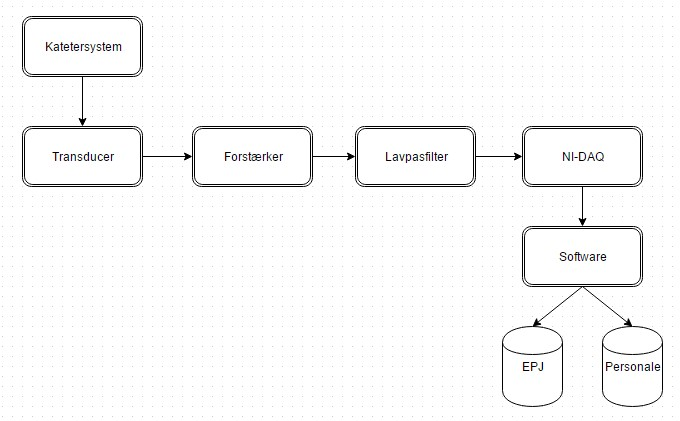
\includegraphics[width =0.8\textwidth , center]{billeder/system}
\caption{\textbf{Skitse af opbygning af systemet.}}
\end{figure}
\newpage
\section{Aktør-kontekst diagram}
\begin{figure}[h!]
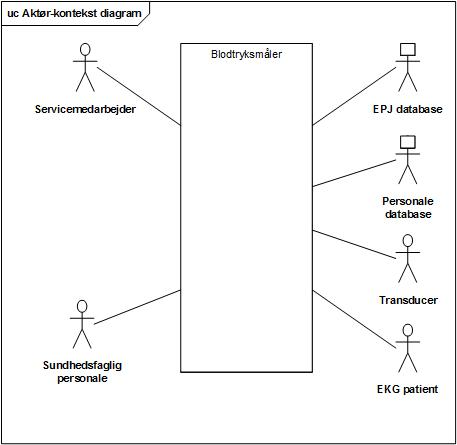
\includegraphics[width =0.65\textwidth , center]{billeder/Aktorkontekst.jpg}
\caption{\textbf{Aktør-kontekst diagram}}
\end{figure}
Af dette diagram ses de interagerende aktører: \textit{Sundhedsfaglig personale}, \textit{Transducer}, \textit{EKG patient}, \textit{EPJ database}, \textit{Personale database} og \textit{Servicemedarbejder}.\\ Herunder er der en detaljeret beskrivelse af hver aktør.
\begin{table}[h!]
\begin{tabular}{| >{\raggedright\arraybackslash}p{3cm} | >{\raggedright\arraybackslash}p{12cm} |}
   \hline
   Navn: & Sundhedsfaglig personale\\ \hline
   Type: & Primær aktør \\ \hline
   Beskrivelse: & Det sundhedsfaglige personale er aktøren, der sætter måleudstyret til transduceren, samt starter målingen. Det er det sundhedsfaglige personale, der interagerer med systemet og dermed har tilgang til de viste målinger på brugergrænsefladerne (startskærm og hovedskærm).\\ \hline
\end{tabular}
\end{table}
\begin{table}[h!]
\begin{tabular}{| >{\raggedright\arraybackslash}p{3cm} | >{\raggedright\arraybackslash}p{12cm} |}
   \hline
   Navn: & Transducer\\ \hline
   Type: & Sekundær aktør \\ \hline
   Beskrivelse: & Transduceren er kilden til måleresultaterne, og fungerer dermed som patienten og forbindelsen til systemet. I dette tilfælde er det en in-vitro maskine, der leverer et tryk til transduceren, som sender dette tryk videre til en forstærker, hvorefter signalet sendes igennem et lavpasfilter, for derefter at sendes ind i systemet via NI-DAQ.\\ \hline
\end{tabular}
\end{table}
\begin{table}[h!]
\begin{tabular}{| >{\raggedright\arraybackslash}p{3cm} | >{\raggedright\arraybackslash}p{12cm} |}
   \hline
   Navn: & EKG patient\\ \hline
   Type: & Sekundær aktør \\ \hline
   Beskrivelse: & EKG patienten er den aktør hvorfra værdierne til EKG-kurven fås fra. Dermed er det denne aktør der er kilden til pulsen. Disse værdier hentes fra PhysioBank ATM.\\ \hline
\end{tabular}
\end{table}
\begin{table}[h!]
\begin{tabular}{| >{\raggedright\arraybackslash}p{3cm} | >{\raggedright\arraybackslash}p{12cm} |}
   \hline
   Navn: & Personale database\\ \hline
   Type: & Sekundær aktør \\ \hline
   Beskrivelse: & Personale database er der, hvori det sundhedsfaglige personales login informationer opbevares, hvilket benyttes til at tilgå systemet. \\ \hline
\end{tabular}
\end{table}
\begin{table}[h!]
\begin{tabular}{| >{\raggedright\arraybackslash}p{3cm} | >{\raggedright\arraybackslash}p{12cm} |}
   \hline
   Navn: & EPJ database\\ \hline
   Type: & Sekundær aktør \\ \hline
   Beskrivelse: & EPJ database er den database, hvor patientdata ligger, samt der hvori analyseresultaterne, der opnås ved målingerne i systemet, samt signalerne bliver gemt. Disse data er grafer for EKG, arterietryk, samt talværdier for puls, systole, diastole og middeltryk. Denne EPJ database skal simulere den EPJ database der fungere på sygehusene i virkeligheden.\\ \hline
\end{tabular}
\end{table}
\begin{table}[h!]
\begin{tabular}{| >{\raggedright\arraybackslash}p{3cm} | >{\raggedright\arraybackslash}p{12cm} |}
   \hline
   Navn: & Servicemedarbejder\\ \hline
   Type: & Primær aktør \\ \hline
   Beskrivelse: & Servicemedarbejderen er aktøreren der igangsætter og foretager kalibreringen.\\ \hline
\end{tabular}
\end{table}
\newpage
\section{Use cases}
\begin{figure}[H]
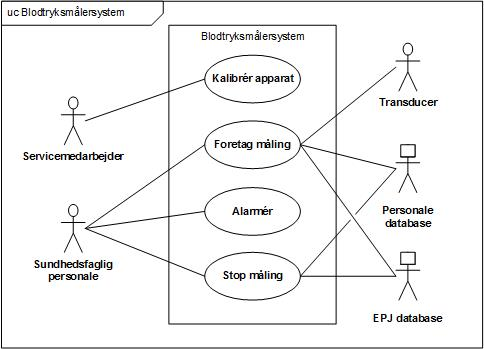
\includegraphics[width =0.7\textwidth , center]{billeder/UseCaseDiagram}
\caption{\textbf{Use case diagram}}
\end{figure}
De fire Use cases kan ses ud fra Use case diagrammet, disse er: \textit{Kalibrér apparat}, \textit{Foretag måling}, \textit{Alarmér} og \textit{Stop måling}. Hver enkel af disse Use cases beskrives detaljeret herunder i et fully-dressed Use case skema.\\
Systemet består af en computer med programkode, en NI-DAQ samt hardware. Hardwaren består af et lavpasfilter, en forstærker og en transducer desuden er der hertil tilkoblet to 9 V batterier.
\\
Systemet gør det muligt at hente data fra det væskefylde kateter via tryktransduceren. Data går herefter fra tryktransduceren igennem forstærkeren, hvilken bliver forsynet af spænding fra to 9 V batterier. Det forstærkede signal fra forstærkeren går videre til lavpasfilteret og derefter ind i NI-DAQ, som så sender data videre til computeren og ind i programkoden. 
\\ 
Det digitale filter er pr. default slået til når systemet startes, dog vil det være muligt at slå dette filter fra under målingen.\\
Når programmet startes skal computeren have VPN-forbindelse til "ASE IHA VPN", desuden skal der være en forbindelse til $"webhotel10.F15ST2ITS2201404669.db_{-}owner"$(Personaledatabasen) og $"webhotel10.F15ST2ITS2201405838.db_{-}owner"$ (EPJ database).\\\\
Programmet skal have to skærme; en startskærm, der fungerer som EPJ systemet, og en hovedskærm, der fungerer som selve blodtryksmålerens grænseflade.

\begin{table}[H]
\caption{Use case 1}\label{tab:tabel4}
\begin{tabular}{| l | >{\raggedright\arraybackslash}p{11cm} |}
   \hline
   \textbf{Use case 1} & \textbf{Kalibrér apparat}\\ \hline
   Mål: & Få kalibreret apparatet \\ \hline
   Initiering: & Startes af Servicemedarbejder\\ \hline
   Aktører:& Servicemedarbejder (primær)\\ \hline
   Referencer: & - \\ \hline
   Samtidige forekomster: & én kalibrering pr. apparat \\\hline
   Forudsætninger: & Blodtryksmålersystemet er tændt og tilsluttet kalibreringsudstyret.\\ \hline
   Resultat:& Apparatet er kalibreret\\ \hline
   Hovedscenarie:& 
\textit{$[$Undtagelse 1: Undlad kalibrering$]$ } \newline
1. Servicemedarbejder foretager kalibreringen, ved at indtaste spændingen og trykket for målepunktet fra væskesøjlen.\newline
2. Systemet beregner kalibreringsværdien.\\\hline
Udvidelse/undtagelser: & \textit{$[$Undtagelse 1:Undlad kalibrering$]$ }\newline
1.1 Undlad kalibrering\newline
1.2 Fortsæt til Use case 2. \newline
1.3 Kalibreringsværdien hentes fra den forrige måling. \\\hline
\end{tabular}
\end{table}


\begin{table}[H]
\caption{Use case 2}\label{tab:tabel5}
\begin{tabular}{| l | >{\raggedright\arraybackslash}p{11cm} |}
   \hline
   \textbf{Use case 2} & \textbf{Foretag måling}\\ \hline
   Mål: & Den valgte patients målinger foretages og værdierne gemmes i EPJ database\\ \hline
   Initiering: & Startes af Sundhedsfaglig personale\\ \hline
   Aktører:& Sundhedsfaglig personale (primær), Personale database (sekundær), EPJ database(sekundær), Transducer (sekundær), EKG patient (sekundær)\\ \hline
   Referencer: & Use case 2 \\ \hline
   Samtidige forekomster: & Én sundhedsfaglig person og én transducer pr. system \\\hline
   Forudsætninger: & VPN, Personale database og EPJ databasen er tilsluttet korrekt\\ \hline
   Resultat:& Målingerne for den valgte patient er foretaget\\ \hline
   Hovedscenarie:& 
1. Sundhedsfaglig personale logger på ved at indtaste brugernavn og kode. \newline
   \textit{$[$Undtagelse 1: Brugernavn og/eller kode indtastet forkert$]$}\newline
2. Besked: "Logget på" vises  \newline
3. Liste med patienter kommer frem\newline
4. Den ønskede patient vælges \newline
5. Sundhedsfaglig personale indtaster nulpunktjusterings værdien og starter nulpunktsjusteringen. \newline
6. Systemet foretager nulpunktsjusteringen. \newline
7. Sundhedsfaglig personale starter målingen \newline
8. Systemet indhenter data fra transduceren og måler, hvor lang tid målingen foretages\newline
9. EKG og arterietryk præsenteres kontinuert på hver sin graf. Puls, systole, diastole og middeltryk vises som talværdier. Data gemmes automatisk løbende i EPJ database. \newline
\textit{$[$Udvidelse 1: Slå digitalt filter til/fra$]$}\newline
\textit{$[$Udvidelse 2: Juster systolens/diastolens grænseværdi$]$}
 \\\hline
Udvidelse/undtagelser: & $[$Undtagelse 1: Brugernavn og/eller kode indtastet forkert$]$\newline
1.1 Besked: "Brugernavn og/eller kode indtastet forkert"\newline
1.2 Use case 3 starter forfra \newline\newline
$[$Udvidelse 1: Slå digitalt filter til/fra$]$\newline 
1.1 Sundhedsfaglig personale vælger "Digitalt filter OFF" \newline
1.2 Systemet slår det digitale filter fra\newline
1.3 Sundhedsfaglig personale vælger "Digitalt filter ON"\newline
1.4 Systemet slår det digitale filter til\newline\newline
$[$Udvidelse 2: Juster systolens/diastolens grænseværdi$]$\newline
2.1 Sundhedsfaglig personale justerer grænseværdierne for systole og/eller diastole.
\\\hline
\end{tabular}
\end{table}

\begin{table}[H]
\caption{Use case 3}\label{tab:tabel6}
\begin{tabular}{| l | >{\raggedright\arraybackslash}p{11cm} |}
   \hline
   \textbf{Use case 3} & \textbf{Alarmér}\\ \hline
   Mål: & Få startet alarmeringen ved overskridelse af en grænseværdi \\ \hline
   Initiering: & Systemet starter denne Use case\\ \hline
   Aktører:& Sundhedsfaglig personale (sekundær)\\ \hline
   Referencer: & Use case 2 \\ \hline
   Samtidige forekomster: & - \\\hline
   Forudsætninger: & Målingen i Use case 2: Foretag måling, er kørt succesfuldt \\ \hline
   Resultat:& Alarmen starter\\ \hline
   Hovedscenarie:& 
1. Grænseværdi overskrides \newline
2. Alarmering starter.\newline
    \textit{$[$Udvidelse 1: Anden grænseværdi overskrides$]$} \newline
    \textit{$[$Udvidelse 2: Udsæt alarm$]$ }\newline
3. Alarmen stopper når grænseværdien ikke længere er overskredet.
\\\hline
Udvidelse/undtagelser: & $[$Udvidelse 1: Anden grænseværdi overskrides$]$ \newline
1.1. Endnu en grænseværdi overskrides\newline
1.2. Første alarm fortsætter, og den nye alarmering igangsætter.\newline
1.3 Use case 3 fortsætter fra punkt 3.\newline\newline
$[$Udvidelse 2: Udsæt alarm$]$\newline
2.1 Sundhedsfaglig person udsætter alarm\newline
2.2 Systemet stopper alarmens lyd i et minut
2.3 Use case 3 fortsætter ved punkt 3.
\\\hline
\end{tabular}
\end{table}

\begin{table}[H]
\caption{Use case 4}\label{tab:tabel7}
\begin{tabular}{| l | >{\raggedright\arraybackslash}p{11cm} |}
   \hline
   \textbf{Use case 4} & \textbf{Stop måling}\\ \hline
   Mål: &  Få stoppet målingen og logget ud\\ \hline
   Initiering: & Startes af Sundhedsfaglig personale \\ \hline
   Aktører: & Sundhedsfaglig personale (primær) \\ \hline
   Referencer: & Use case 2\\ \hline
   Samtidige forekomster: & - \\\hline
   Forudsætninger: & Use case 2: Foretag måling, er kørt succesfuldt\\ \hline
   Resultat:& Signalet er stoppet, sundhedsfaglig personale er logget ud og vendt tilbage til startskærm.\\ \hline
   Hovedscenarie:& 
1. Sundhedsfaglig personale stopper måling\newline
2. Systemet stopper målingen.\newline 
3. Sundhedsfaglig personale logger ud \\\hline
Udvidelse/undtagelser: & -\\\hline
\end{tabular}
\end{table}
\newpage 
\newpage 
\newpage
\newpage
\section{Ikke-funktionelle krav}
De ikke-funktionelle krav er opsat efter FURPS+ metoden. De er prioriteret efter MoSCoW metoden:
\begin{itemize}
\item \textbf{M}ust (skal være med)
\begin{itemize}
\item De krav der dermed bliver markeret med et \textbf{(M)}, er altså de krav til funktioner der skal være til produktet.
\end{itemize}
\item \textbf{S}hould (bør være med, hvis muligt)
\begin{itemize}
\item Kravene kan også markeres med et \textbf{(S)}. Disse krav er funktioner produktet bør have.
\end{itemize}
\item \textbf{C}ould (kunne have med, hvis det ikke går i vejen for noget andet)
\begin{itemize}
\item Markeres et krav med \textbf{(C)}, behøver produktet ikke at have funktionen, men det kunne være en funktion der kunne være god at have til produktet.
\end{itemize}
\item \textbf{W}on't/\textbf{W}ould (tager det ikke med nu, men kan komme med i fremtidige opdateringer)
\begin{itemize}
\item Dermed er de krav der bliver markeret med et \textbf{(W)}, altså de krav til funktioner der ville være gode til produktet, men ikke bliver implementeret i produktet. Grunden til dette kan være at der ikke er tid, eller at funktionen ikke er vigtig for produktet.
\end{itemize}
\end{itemize}
\subsection{FURPS+ med MoSCoW}
\begin{enumerate}
\item \textbf{Functionality}
\begin{enumerate}
\item (\textbf{M}) Programmet skal have et digitalt filter til udglatning af blodtrykssignal.
\item (\textbf{S})Programmet skal give alarm, når grænseværdier for blodtrykket overskrides, med lyd og "Udsæt alarm" knappen blinker skiftevis mellem rød og hvid.
\item (\textbf{M}) Programmet skal kunne gemme blodtrykssignalet i en database.
\end{enumerate}
\item \textbf{Usability}
\begin{enumerate}
\item (\textbf{S}) Programmet skal have to window forms: startskærm, der fungerer som  EPJ systemet og hovedskærm, der fungerer som selve blodtryksmålerens grænseflade.
\item (\textbf{M}) Programmet skal have en "Log ind" knap på startskærmen.
\item (\textbf{M}) Programmet skal have en "Kalibrering" knap på startskærmen.
\item (\textbf{M}) Sundhedsfagligt personale skal kunne ændre "devicename/enhedsnavn" i dropdown på startskærmen.
\item (\textbf{S}) Programmet skal indeholde en dropdown, hvor patienten kan vælges, på startskærmen.
\item (\textbf{M}) Programmet skal have en "Nulpunkts indstilling" knap på hovedskærmen.
\item (\textbf{M}) Programmet skal have to radiobuttons til at slå det digitale filter fra og til på hovedskærmen.
\item (\textbf{S}) Programmet skal have knapper til at justere systolisk og diastolisk grænseværdi-intervaller op og ned, på hovedskærmen.
\item (\textbf{S}) Programmet skal have en "Udsæt alarm" knap på hovedskærmen.
\item (\textbf{M}) Programmet skal have en "Tænd" knap på hovedskærmen.
\item (\textbf{M}) Programmet skal have en "Sluk" knap på hovedskærmen.
\item (\textbf{M}) Programmet skal have en "Log ud" knap på hovedskærmen.
\item (\textbf{M}) Teksten på startskærmen skal kunne læses fra 2 meters afstand ved synsstyrke i intervallet på +/-1.
\item (\textbf{M}) Teksten og graferne på hovedskærmen skal kunne læses fra 2 meters afstand ved synsstyrke i intervallet på +/-1.
\item (\textbf{M}) Programmet skal præsentere arterietryk kontinuert, herudover vise systolisk værdi, diastolisk værdi og middeltryk som talværdier.
\item (\textbf{S}) Programmet skal præsentere EKG og puls.
\item (\textbf{W}) Programmet skal præsentere iltmætning både som graf og talværdi.
\item (\textbf{M}) Programmet skal præsentere data på grafer på følgende måde (Se afsnit nedenfor).
\begin{itemize}
\item EKG vises i lysegrøn.
\item Arterietryk vises i rød.
\item Iltmætning/saturation i lyseblå.
\end{itemize}
\item (\textbf{M}) Programmet skal præsentere data i tal på følgende måde (Se afsnit nedenfor)
\begin{itemize}
\item Hjertefrekvens (puls) i lysegrøn.
\item Systolisk samt diastolisk tryk i rødt, ligeledes middelblodtrykket i parentes ved siden af i rødt.
\item Iltmætningsværdien i lyseblå.
\end{itemize}
\begin{figure}[h!]
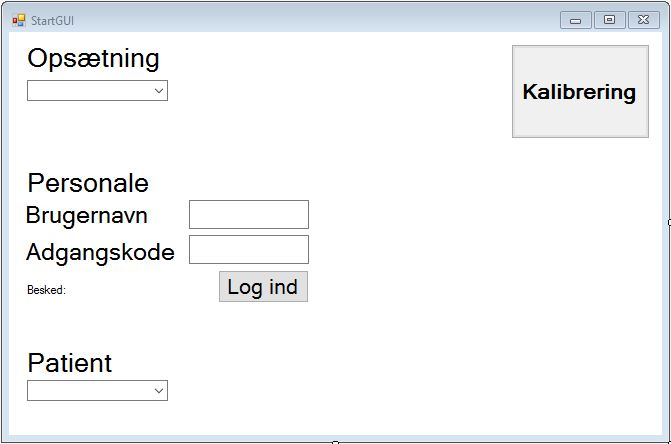
\includegraphics[width =0.4\textwidth , center]{billeder/skitseStart}
\caption{Skitse af startskærmen, som repræsenterer EPJ systemet}
\end{figure}
\begin{figure}[h!]
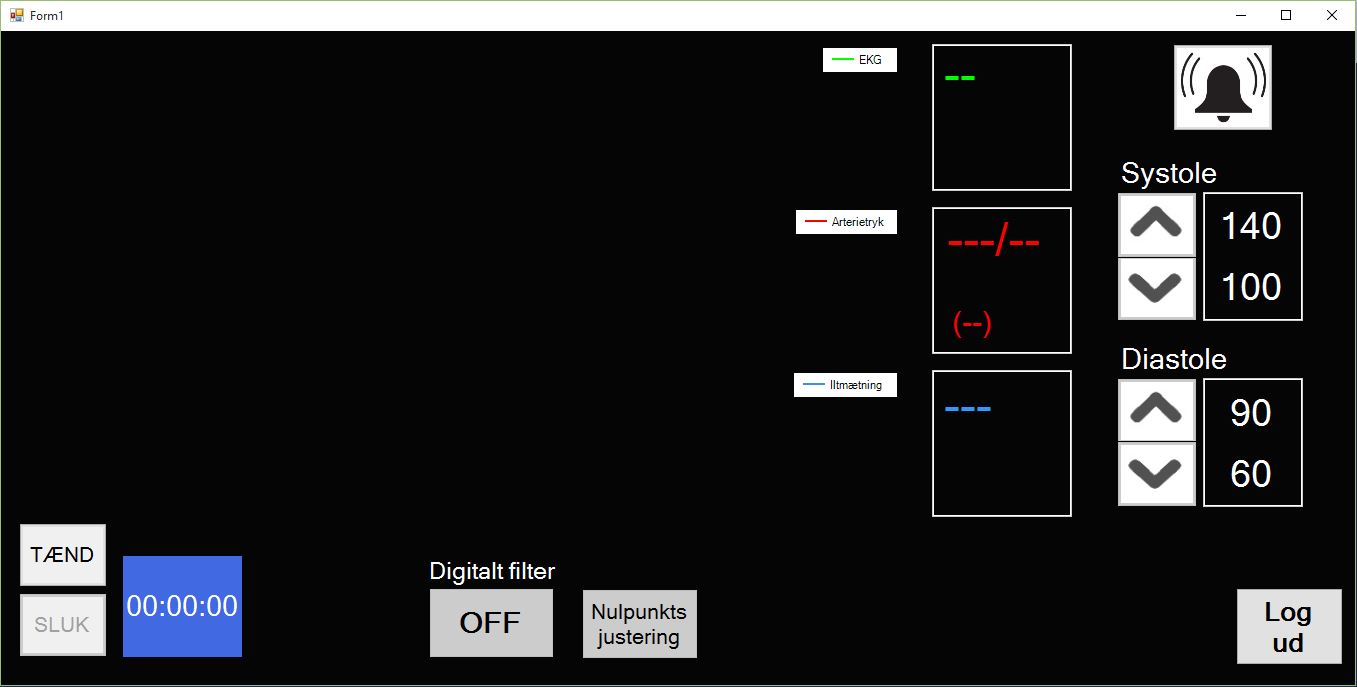
\includegraphics[width =1.0\textwidth , center]{billeder/skitseHoved}
\caption{Skitse af hovedskærmen, hvilken repræsenterer en blodtryksmålers brugergrænseflade}
\end{figure}
\end{enumerate}
\item \textbf{Reliability}
\begin{enumerate}
\item (\textbf{S}) INGEN RELIABILITY KRAV ENDNU
\end{enumerate}
\item \textbf{Performance}
\begin{enumerate}
\item (\textbf{S}) Tiden der går før måling af data påbegynder/vises i grafer må maksimalt være 2 sek.
\item (\textbf{S}) Tiden der går fra at data, herunder puls, diastolisk tryk, systolisk tryk og middeltryk, er analyseret til at data er gemt i EPJ database må være 2 sek. med en tolerance på +/-15\% 
\item (\textbf{S}) Ved justering af grænseværdi for systole og diastole ændres grænseværdien 1 mmHg op eller ned.                                                                                                                                                                                                                                                                                                                                                                                                                                                                                                                                                                                                                                                                                               
\end{enumerate}
\item \textbf{Supportability}
\begin{enumerate}
\item (\textbf{M}) Programmet skal skrives i C\# kode
\item (\textbf{M}) Softwaren skal være opbygget efter trelagsmodellen (Data-View-Model)
\item (\textbf{S}) I softwaren benyttes Observer/Subject mønsteret.
\item (\textbf{S}) I softwaren benyttes PUSH mønsteret
\end{enumerate}
\item \textbf{+ Test conditions}
\begin{enumerate}
\item (\textbf{M}) Der skal være adgang til en computer med Windows 7, 8 eller 10 - computeren skal minimum have 4 GB RAM.
\item (\textbf{M}) Der skal være adgang til en computer hvor National Instruments er installeret.
\end{enumerate}
\end{enumerate}
\chapter{Arkitektur og design}
Følgende beskriver arkitekturen for systemet herunder både hardware og software. 
Systemarkitektur er udviklingsrammen for den videre udvikling af design og implementering. Der vil igennem dette afsnit startes med at se systemet overordnet og hvorefter der arbejdes ned gennem systemet i mindre brudstykker. Der benyttes diagrammer for at kunne specificere og klarlægge systemkravene. Disse diagrammer beskrives desuden i tekst. Igennem dette afsnit bliver designet af produktet dermed bestemt.
\section{Hardware design}
\subsection{Udviklingsfase og iterationer}
I dette afsnit redegøres der for udviklingsprocessen på hardware-teamet, som har bestået af tre mand. Der redegøres for de løsnings-iterationer gruppen har været igennem, samt gruppens tankeproces mens der er arbejdet på projektet. Udviklingen af hardwaren til projektet har foregået som et teknologistudie baseret på krav til projektet og tidligere viden fra Analog Signal Behandling. Processen har været en iterativ og agil udviklingsproces, som er præget af en generel mangelfuld viden på området.
\subsubsection{Første iteration - komponenter i lavpasfilteret}
Der blev besluttet, at tage udgangspunkt i beregningsværktøjer på nettet \cite{filter}  til den første iteration. Dette gav nogle værdier der lå meget tæt på det ønskede resultat. Kredsløbet blev derefter bygget op på et fumlebræt og fastsatte komponent værdierne ud fra beregningerne fra nettet. Udregningen fra nettet var baseret på en cut-off frekvens på 50Hz og C1 $=$ C2.
\begin{figure}[H]
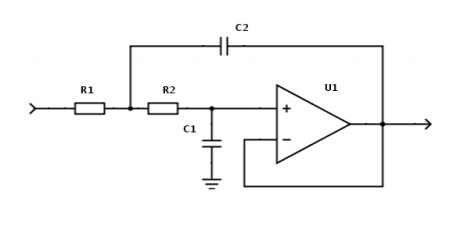
\includegraphics[width =0.5\textwidth , center]{billeder/butterworth}
\caption{\textbf{Butterworth Sallen-key filter.}}
\end{figure}
\begin{table}[H]
\begin{tabular}{| l | l |}
   \hline
   Komponent & Værdi\\ \hline
   R1 & 4.7 $k\Omega$ \\ \hline
   R2 & 4.7 $k\Omega$ \\ \hline
   C1 & 680 nF\\\hline
   C2 & 680 nF\\\hline
\end{tabular}
\end{table}
Det viste sig at det ikke levede op til kravene omkring den nødvendige dæmpning ved 500Hz, ligeledes opførte filteret sig ikke som ønsket. I starten var der blandt andet arbejdet med filteret som passivt, noget som der først fik rettet op på til sidste iteration. Desuden fik hjælpen fra en ASB-underviser, vist at ovenstående filter ikke overholdte kravene til et 2. ordens Butterworth Sallen-key filter. 
\subsubsection{Anden iteration - komponenter i lavpasfilteret}
Den anden iteration er beskrevet udførligt i hardware delen, her blev der brugt en mere matematisk proces til at designe filteret. Der blev gættet på en C1 værdi på 330nF, og herefter blev de resterende komponentværdier skaleret ud fra dette. Neden for ses de udregnede komponentværdier for lavpasfilteret version 2.
\begin{table}[H]
\begin{tabular}{| l | l |}
   \hline
   Komponent & Værdi\\ \hline
   R1 & 6.7 $k\Omega$ \\ \hline
   R2 & 6.7 $k\Omega$ \\ \hline
   C1 & 330 nF\\\hline
   C2 & 680 nF\\\hline
\end{tabular}
\end{table}
Filteret blev analyseret. Analysen viste, at der ikke kom den nødvendige dæmpning ved 500Hz. Igen kan dette være et resultat af det ikke var aktivt. 
\subsubsection{Tredje iteration - komponenter lavpasfilteret, forstærker og forsyningsspænding}
I den tredje iteration blev der opdaget at C1 skulle være halvdelen af C2 for at give et filter der overholdte projektets krav. Modstandene er beregnet ud fra den nye kondensatorværdi.
\begin{table}[H]
\begin{tabular}{| l | l |}
   \hline
   Komponent & Værdi\\ \hline
   R1 & 6.6 $k\Omega$ \\ \hline
   R2 & 6.6 $k\Omega$ \\ \hline
   C1 & 340 nF\\\hline
   C2 & 680 nF\\\hline
\end{tabular}
\end{table}
Der blev besluttet at benytte en INA-114 forstærker, efter anbefaling fra vejleder og medstuderende. Der blev beregnet forstærkningen, samt blev der sikret at forstærkeren opfyldte projektets krav. Beslutningen om hvilken forsyningsspænding der skulle benyttes, faldt på to 9V-batterier. Det blev undersøgt hvorvidt det var muligt at bruge andre spændingsforsyninger, blandt andet USB og dedikerede spændingsforsyninger. USB som spændingsforsyning blev fravalgt da der ikke kunne opnå tilstrækkelig forstærkning I INA-114 forstærkeren, så det ville gå ud over præcisionen. De udleveret spændingsforsyninger blev fravalgt af praktiske årsager, da de var meget uhåndterbare.
\subsubsection{Fjerde iteration - aktivt filter}
Den fjerde iteration benytter samme komponentværdier som tredje iteration, men det var blevet overset at filteret skulle være aktivt. Derfor blev der bygget et kredsløb op forfra på fumlebræt, hvor der var tilsluttet spænding på filteret.
\subsubsection{Design af lavpasfilteret}
Frekvenserne der skal arbejdes med i blodtryksmåleren, ligger op til 50Hz, derfor skal der realiseres et 2. ordens lavpasfilter med følgende dimensioner:\\
Cut-off Frequency: 50Hz\\
Ligeledes skal der dæmpes med 40 dB/decade ved 500Hz.\\
C2 er givet til at være på 680nF, ligeledes er operationsforstærkeren givet til at være OP27.
\begin{figure}[H]
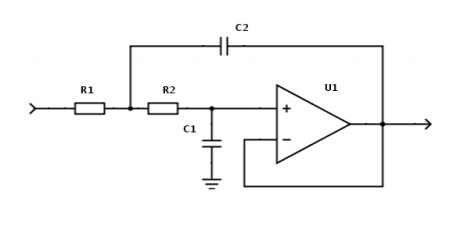
\includegraphics[width =0.5\textwidth , center]{billeder/lavpas}
\caption{\textbf{Butterworth Sallen-key filter.}}
\end{figure}
Overføringsfunktionen for ovenstående filter:
\begin{align}
\dfrac{V_{out}(s)}{V_{in}(s)}=\dfrac{\dfrac{1}{R1\cdot R2\cdot C1\cdot C2}}{s^2+\dfrac{R1 + R2}{R1\cdot R2\cdot C2}\cdot s+\dfrac{1}{R1\cdot R2\cdot C1\cdot C2}}
\end{align}
Omskrevet til standardformel:
\begin{align}
\dfrac{V_{out}(s)}{V_{in}(s)}=\dfrac{\omega^2}{s^2+2\zeta\omega+\omega^2}
\end{align}
Her isoleres cut-off frekvensen ($\omega$) i overføringsfunktionen for lavpasfilteret:
\begin{align}
\omega = 2\pi\sqrt{\dfrac{1}{R1\cdot R2\cdot C1\cdot C2}}
\end{align}
I formlen for cut-off frekvensen indsættes komponentværdierne. Der er valgt en værdi for $C1$ til at være 330nF, dette er et gæt. Cut-off frekvensen er sat til 50Hz, da dette er blevet givet som et krav til projektet.\\
$C1 = 330nF, C2=680nF og R1=R2$
\begin{figure}[H]
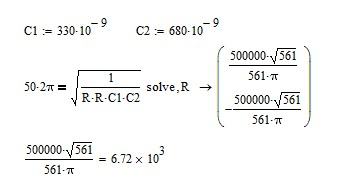
\includegraphics[width =0.5\textwidth , center]{billeder/mathcad}
\caption{\textbf{Mathcad beregninger.}}
\end{figure}
Ud fra disse beregninger skal modstanden altså bestemmes til at have en værdi på ca. $6.7k\Omega$. Da der er blevet brugt et Butterworth Sallen-key filter vides der, at C1 skal være halvdelen af C2. Derfor er der lavet nye beregninger hvor $C1=340nF$, hvilket svarer til halvdelen af $C2$.
\begin{figure}[H]
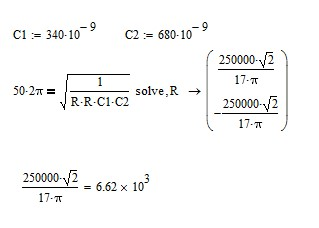
\includegraphics[width =0.5\textwidth , center]{billeder/mathcad2}
\caption{\textbf{Mathcad beregninger.}}
\end{figure}
Der er efterfølgende lavet en analyse i matlab for at sikre at dæmpningen er min. 40 dB pr. decade ved 500Hz. Dette er gjort med modstande på $6.6k\Omega$.
\begin{figure}[H]
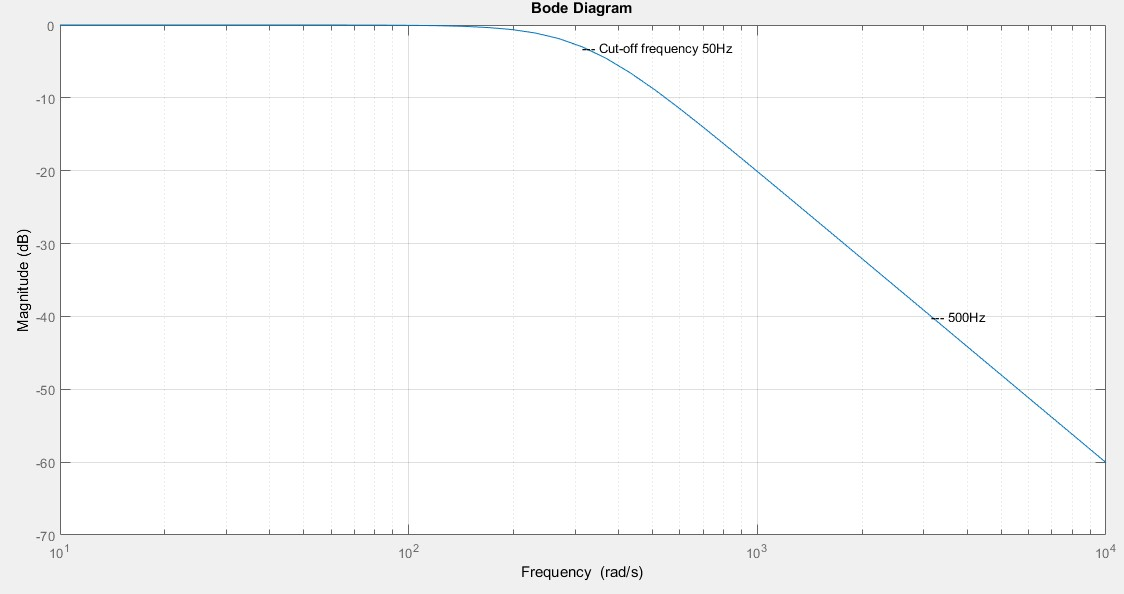
\includegraphics[width =1.0\textwidth , center]{billeder/bodeplot}
\caption{\textbf{Matlab bodeplot med 6.6k$\Omega$ modstande.}}
\end{figure}
Ud fra dette kan det konkluderes at dæmpningen ved 550Hz er tilstrækkelig.
\subsubsection{Design af operationsforstærkeren}
Det elektriske signal der skal bruges i systemet, kommer fra tryktransduceren TruWave\texttrademark og ind i dataopsamlingsmodel (NI-DAQ6009). Signalet fra TruWave\texttrademark skal forstærkes op, så der kommer bedre målesignaler i DAQ’en. I databladet for NI-DAQ6009 kan der ses den maksimale spænding for indgangsportene er +/-10V, det vil sige at der ikke må forstærkes mere op end 10V. Der er valgt at forstærke op til +/-8V, for at give lidt buffer, så der ikke overstiges de 10V og derved mister data. Ligeledes er "projektet" hæmmet af valget af strømforsyning som er to 9-volts batterier, som praktisk leverer omkring +/- 8V.\\ 
Fra TruWave\texttrademark er der valgt at fokuserer på et måleområde der hedder 0-250mmHg. \\\\
\textbf{Maksimalt output for transducer}\\
\begin{align}
V_{max}=250mmHg\cdot 16V\cdot 5\mu V 
\end{align}
Ud fra dette kan der bestemmes, hvor meget gain (forstærkning), der skal bruges fra forstærkeren:
\begin{align}
16V = 20\cdot 10^{-3}V\cdot gain\\
gain = \dfrac{16V}{20\cdot 10^{-3}V}=800
\end{align}
\textbf{Båndbredde og valg af forstærker}\\
Produktet af gain og båndbredde, $BW$, er konstant, derfor er det vigtigt vores båndbredde ligger over knækfrekvensen på 50Hz. Der er valgte at benytte en INA-114 forstærker da den opfylder behovene. Ved $gain=1$ kan INA-114 levere 1MHz båndbredde, det vil sige, at der kan opstilles følgende ligning for beregning af båndbredden.
\begin{align}
1000000 = 800\cdot BW\\
BW = \dfrac{1000000Hz}{800}=1250Hz
\end{align}
Da 1250 Hz er over knækfrekvensen på 50Hz har forstærkeren tilstrækkelig båndbredde til at leve op til kravene til projektet.\\\\
\textbf{Beregning af modstand til forstærker}\\
\begin{figure}[H]
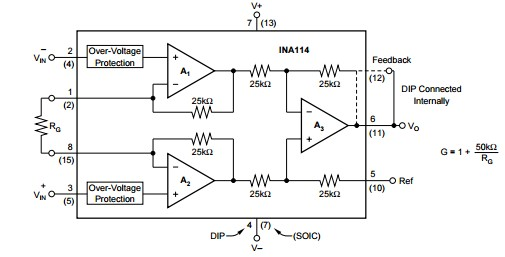
\includegraphics[width =1.0\textwidth , center]{billeder/forstarker}
\caption{\textbf{Denne viser opbygningen og delene i operationsforstærkeren INA114}}
\end{figure}
Forstærkerens gain er bestemt ved modstanden der sidder på port 1 og 8. Denne modstand kan beregnes med følgende formel, hvor $R_G$ er modstanden og gain = 800.
\begin{align}
G=1+\dfrac{50k\Omega}{R_G}\\
800 = 1+\dfrac{50k\Omega}{R_G}\\
R_G=62.5\Omega
\end{align}
Et potentiometer er blevet valgt at benytte som denne modstand, da der helst skulle kunne reguleres på systemet, og den ovenstående værdi er beregnet med ideelle komponenter.
\subsection{Implementering}
\subsubsection{Block definition diagram}
På nedenstående figur bliver systemets hardware illustreret i et BDD. Heraf ses det at systemet har seks hardware blokke: Computer, transducer, NI-DAQ, lavpas filter, forstærker og en strømforsyning. Disse blokke udgør tilsammen blodtryksmålersystemet.
\begin{figure}[H]
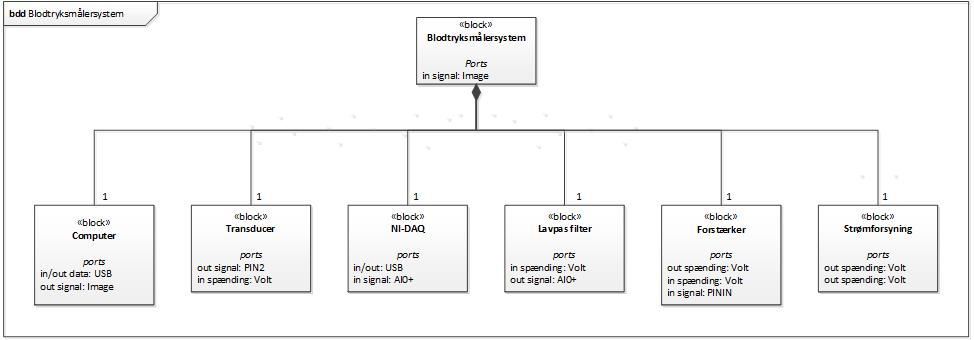
\includegraphics[width =1.0\textwidth , center]{billeder/BDD}
\caption{\textbf{Block definition diagram. Dette diagram viser hardware delene i systemet, samt sammenhængen mellem disse.}}
\end{figure}
\subsubsection{Internal block definition}
Ud fra BDD kan et IBD diagram udarbejdes. IBD diagrammet viser koblingen mellem blokkene:
\begin{itemize}
\item Strømforsyningen, denne er to 9V batterier som forsyner forstærkeren og transduceren med $\pm$ 9V
\item Transduceren omdanner tryksignalet fra kateteret til et strømsignal i ZZ mV tilbage til forstærkeren.
\item Forstærkeren forstærker signalet til lavpas filteret.
\item Lavpas filteret dæmper de høje frekvenser og sender signalet til NI-DAQ
\item NI-DAQs formål er, at omdanne signalet fra et analogt signal til et digitalt signal.
\item Computerens funktion er at få analyseret og vist blodtryksignalet på en brugergrænseflade, vha. Visual Studio. 
\end{itemize}
\begin{figure}[H]
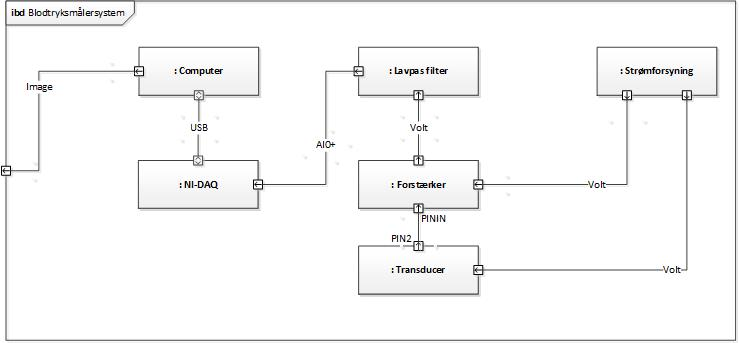
\includegraphics[width =1.0\textwidth , center]{billeder/IBD}
\caption{\textbf{Internal block diagram. Dette diagram viser signalerne imellem blokkene.}}
\end{figure}
\subsection{Modultest}
Modultesten omfatter kun en operationsforstærker. De resterende komponenter, som er anvendt i den samlede hardwaresystem, tages ikke i modultesten, da de er udleverede af vejlederen. De udleverede dele af systemet består af et filter, en transducer, et kateter og en dataopsamler i form af NI-USB-6009. Selvom filtret er udleverede, indgår den i modultesten, da man skal sikre at det dæmper de høje frekvenser.  Modultesten foretages enkeltvis dvs. de enkelte blokke testes hver for sig. Til sidst testes systemet med en vandsøjle for at identificere om operationsforstærkeren og filteret kommunikere med hinanden. Rækkefølgen som blokkene skal testes er som følgende:
\begin{itemize}
\item Test af operationsforstærker.
\item Test af filter.
\item Den enelige test med vandsøjle.
\end{itemize}
\begin{figure}[H]
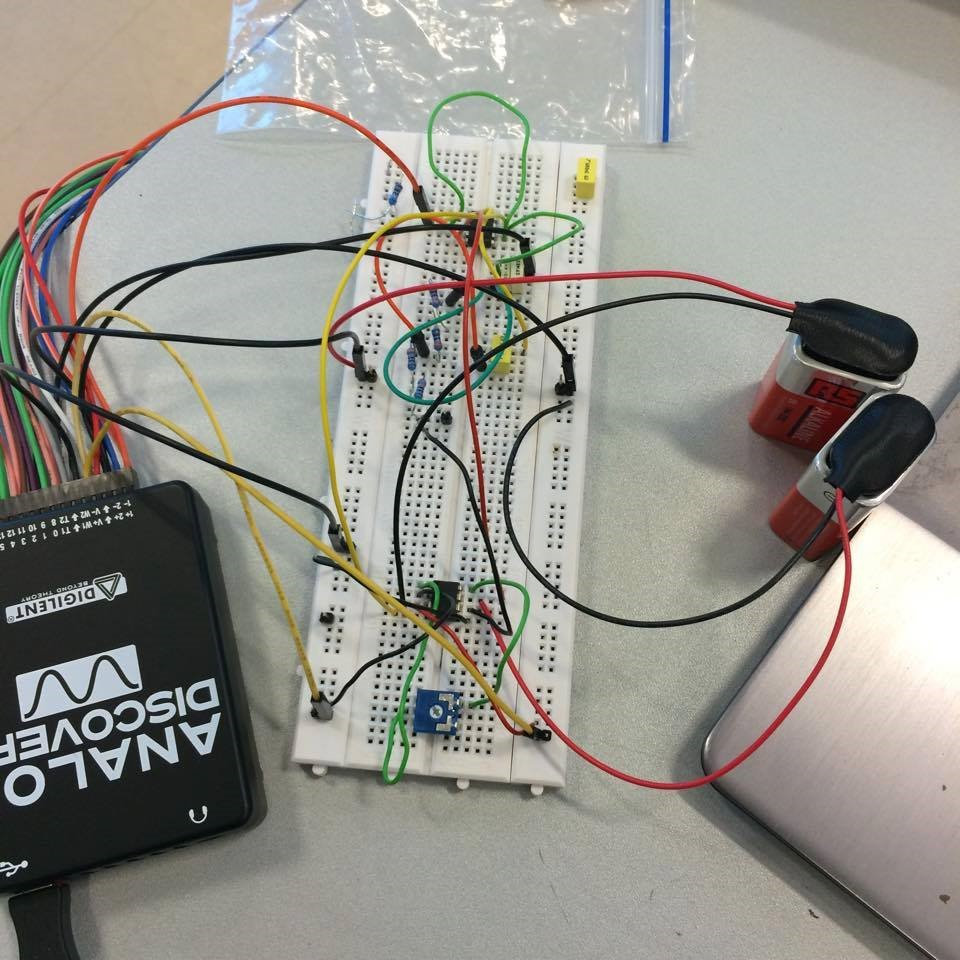
\includegraphics[width =1.0\textwidth , center]{billeder/testOpstilling}
\caption{\textbf{Opstilling af hardware systemet simuleret med Analog Discovery.}}
\end{figure}
\subsubsection{Test af operationsforstærker} 
Operationsforstærkerens funktion er at forstærke et lavt signal til et ønsket højt signal. Der er brugt INA-114 som operationsforstærker, da det er muligt at få den ønskede forstærkning ved den ønskede båndbredde. Der er i alt 8 pin og det forklares som følgende:
\begin{table}[H]
\label{tab:tabel2}
\begin{tabular}{| l | l |}
   \hline
   Pin 1 = $R_{G}$ & Pin 5 = $Ref$ \\ \hline
   Pin 2 = $V_{in}^{-}$ & Pin 6 = $V_{0}$\\ \hline
   Pin 3 = $V_{in}^{+}$ & Pin 7 = $V^{+}$\\ \hline
   Pin 4 = $V_{-}$ & Pin 8 = $R_{G}$\\ \hline
\end{tabular}
\end{table}
\begin{figure}[H]
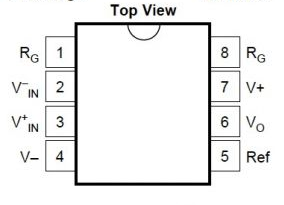
\includegraphics[width =0.2\textwidth , center]{billeder/ina_114}
\caption{\textbf{Op. Amp. INA-114}}
\end{figure}
Vha. Analog Discovery er der påført INA-114 et differentielt signal dvs. to signaler med hver 10mV, hvor der varieres i frekvensen fra 1 til 500Hz. Det forventet resultat er at de 20mV bliver forstærket. De to signaler har samme stelpunkt. Outputtet af signalet måles vha. et oscilloskop. Resultatet af denne simulering er som følgende:
\begin{table}[H]
\label{tab:tabel2}
\begin{tabular}{| l | l |}
   \hline
   Frekvens [Hz] & Forstærket [V]. Peak to peak.  \\ \hline
   1 & 16,308 \\ \hline
   10 & 17,512\\ \hline
   25 & 17,558 \\ \hline
   49 & 17,512 \\\hline
   70 & 17,258 \\\hline
  100 & 17,308 \\\hline
\end{tabular}
\end{table}
\subsubsection{Test af filter}
Systemets filtre er et 2. ordens lavpasfilter af typen Sallen-Key og designes som et Butterworth med cut off frekvens på 50Hz. Om filtret lever op til de opstillet krav kan testes ved at sende signaler med høje frekvenser igennem. De høje frekvenser skal blive dæmpet. Der er brugt Analog Discovery til at generer et signal med forskellige frekvenser. Da cut off frekvensen ligger på 50Hz, forventes der at alt over 50 bliver dæmpet og ved 500 skal der dæmpes minimum 40 dB pr. dekade.
\begin{table}[H]
\label{tab:tabel2}
\begin{tabular}{| l | l |}
   \hline
   Frekvens [Hz] & Spænding [V] \\ \hline
   1 & 13,504 \\ \hline
   10 & 13,220\\ \hline
   25 & 12,412 \\ \hline
   49 & 10,644 \\\hline
   70 & 6,658 \\\hline
   100 & 3,662 \\\hline
   250 & 0,666 \\\hline
   500 & 0,220\\\hline
\end{tabular}
\end{table}
Nedstående figur viser et meget lille signal input på 20mV. De 20 mV bliver herefter forstærket til 10,854V. Dette tal er ikke en 11 volts forstærkning, men peak to peak forstærkning. 
\begin{figure}[H]
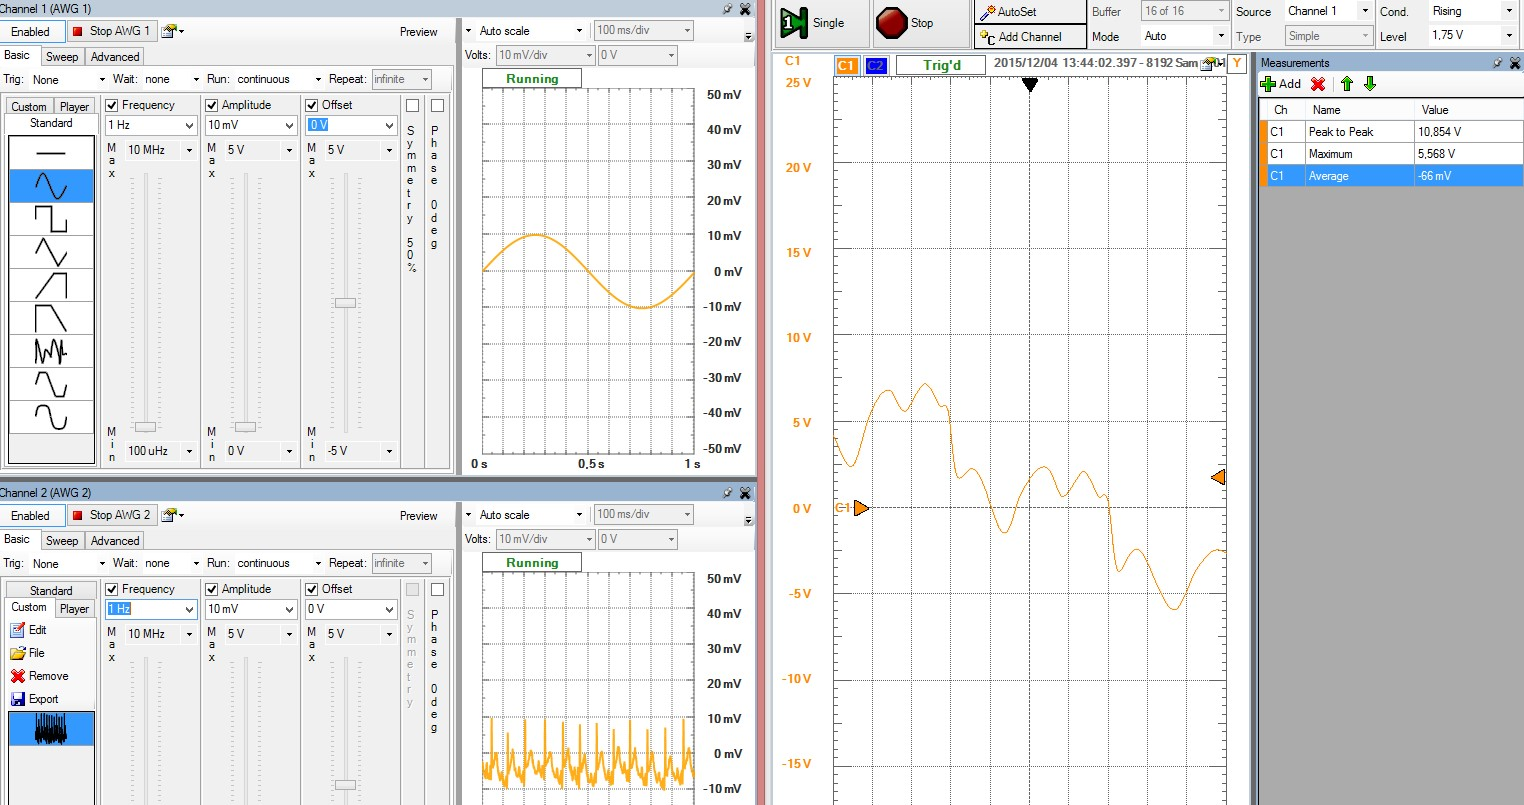
\includegraphics[width =1.0\textwidth , center]{billeder/testFilter}
\caption{\textbf{Output af lavpasfilteret ved 1 Hz.}}
\end{figure}
\subsubsection{Test med vandsøjle}
Den endelig måling er foretages vha. vandsøjlen som signalgenerator i form af tryk til transduceren. Det generede signal skal herefter igennem forstærkeren, hvor der forventes at operationsforstærkeren forstærker signalet. Tabellen viser trykket fra vandsøjlen til transduceren og det forstærket tryk i V. Nedstående målinger er det der er kalibrereret efter. Hældning af den nedstående kurve er kalibreringskoefficienten i V/mmHg. For at lave det om til mmHg/V skal hældning ganges med 30,21 ved fx tryk på 10mmHg. 
\begin{table}[H]
\label{tab:tabel2}
\begin{tabular}{| l | l |}
   \hline
   Tryk [mmHg] & Spænding [V] \\ \hline
   0 & 0,147 \\ \hline
   10 & 0,478\\ \hline
   50 & 2,025 \\ \hline
   100 & 3,601\\\hline
\end{tabular}
\end{table}
\begin{figure}[H]
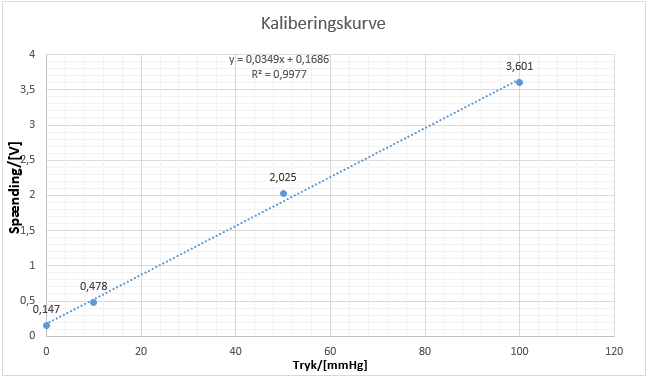
\includegraphics[width =1.0\textwidth , center]{billeder/vandsojleTest}
\caption{\textbf{Sammenhængen mellem tryk og spænding.}}
\end{figure}
\newpage
\section{Software design}
I dette afsnit beskrives softwaredesign på baggrund af systembeskrivelsen og kravspecifikationen. Denne beskrivelse opnås ved, at der benyttes relevante diagrammer og modeller, hvilke kan bruges til at beskrive softwaren. Overvejelser og valg, der er blevet gjort i forbindelse med design og implementering af softwaren, vil i dette afsnit blive præsenteret.
\subsection{Problemidentifikation}
Ved identifikationen af produktet, og herunder hvad dette skal kunne, er der opstået nogle vanskeligheder, som der har skullet tages hensyn til. I første omgang blev der udarbejdet en idé, om at have en startskærm, hvor det kunne vælges hvorpå målingen skulle foretages. På startskærmen skulle det desuden være muligt at kalibrere systemet og foretage nulpunkts justeringen. Stederne hvor målingerne skulle foretages blev identificeret til at skulle være tre målesteder; hjertet, armen og benet. Efter målestedet var valgt, skulle man komme videre til en anden skærm, hvor selve målingen skulle foretages. Idé med denne startskærm viste sig dog ikke at være brugbar i praksis, hvilket fik os til at gå væk fra denne. Grunden til at denne idé ikke ville kunne bruges i praksis, ved en invasiv blodtryksmåling, var at denne idé var tænkt som et produkt til måling af blodtrykket på diabetes patienternes underekstremiteter. Herefter ville værdierne kunne sammenlignes, og situationen vurderes for patienten. Men ved denne patientgruppe er det dog ikke hensigtsmæssigt at lave invasiv blodtryksmåling på underekstremiteterne, da blodtrykket her vil være lavt. Ved invasiv blodtryksmålingen laves der hul på karrene og helingen af dette hul vil ikke kunne foregå optimalt og der vil være risiko for infektioner. \\
\begin{figure}[H]
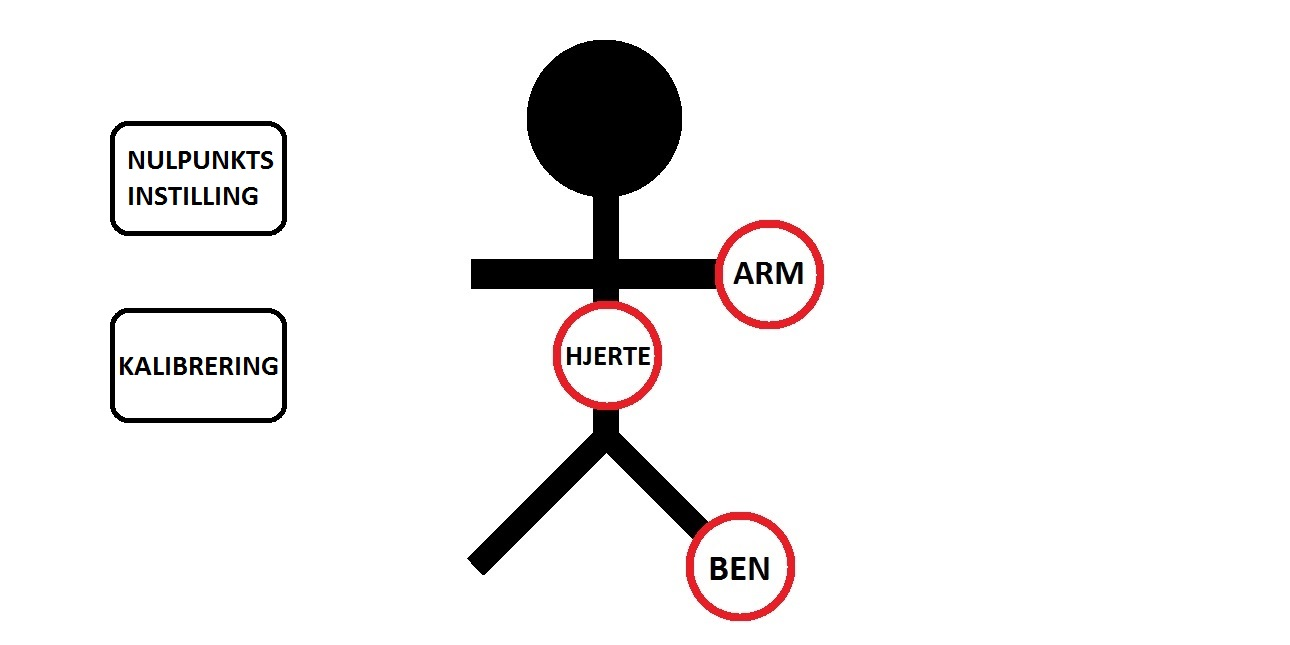
\includegraphics[width =0.5\textwidth , center]{billeder/SkitseStartGammel}
\caption{\textbf{Idé til projekt. Startskærmen hvor det vil være muligt at vælge målested.}}
\end{figure}
Herefter blev idéen ændret til et produkt, der ligner det der fungerer i dagligdagen på hospitalerne. Denne idé blev udarbejdet efter et besøg på Herning Sygehus, hvor et møde med anæstesi sygeplejerske Charlotte Høj blev afholdt. Her blev det muligt at se et scenarie med en blodtryksmåling. Ved scenariet loggede Charlotte Høj først ind på EPJ computeren, hvorefter selve blodtryksmålingen kunne foretages fra en anden skærm.\\
Ud fra denne idé blev en startskærm, som skal simulere EPJ-systemet (EPJ computeren), udarbejdet. EPJ-systemet er der, hvor det sundhedsfaglige personale kan tilgå patientens data, og dermed evt. se hvilket behandling patienten har været igennem før. Startskærmen der her er udarbejdet, er blot en prototype af dette og derfor er det kun den del, hvor det sundhedsfaglige personale logger på, samt vælger patient, der er blevet implementeret. Dermed er det ikke muligt at tilgå tidligere behandlinger osv. Desuden blev nulpunkts justeringen, hvilken hertil var placeret på startskærmen, flyttet ind på hovedskærmen, altså skærmen, hvor selve målingen foretages. Dette blev denne, da der var en antagelse om at der skulle sendes et signal igennem systemet før denne kunne foretages. Dog er det senere blevet klart at dette ikke er aktuelt, idet denne sagtens kan udføres før ved denne prototype. Kalibreringen foretages med en væskesøjle, hvor der er tre punkter, som fører til at en spænding kan aflæses. Ud fra det tryk der leveres af væskesøjlen samt den målte spænding, kan en hældningskoefficient bestemmes, hvilken systemet skal gemme til at regne på alle data.\\
Ud fra alle disse faktorer kan grundstrukturen, til hvordan startskærmen og hovedskærmen skal se ud, dannes:
\begin{figure}[H]
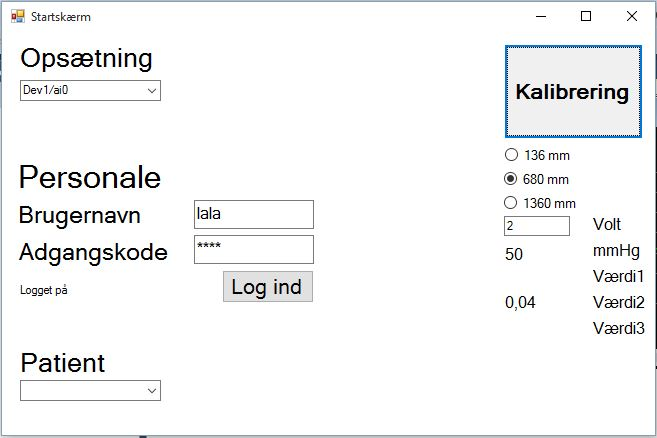
\includegraphics[width =0.5\textwidth , center]{billeder/SkitseStartNy}
\caption{\textbf{Startskærmen, hvilken fungerer som EPJ-systemet}}
\end{figure}
\begin{figure}[H]
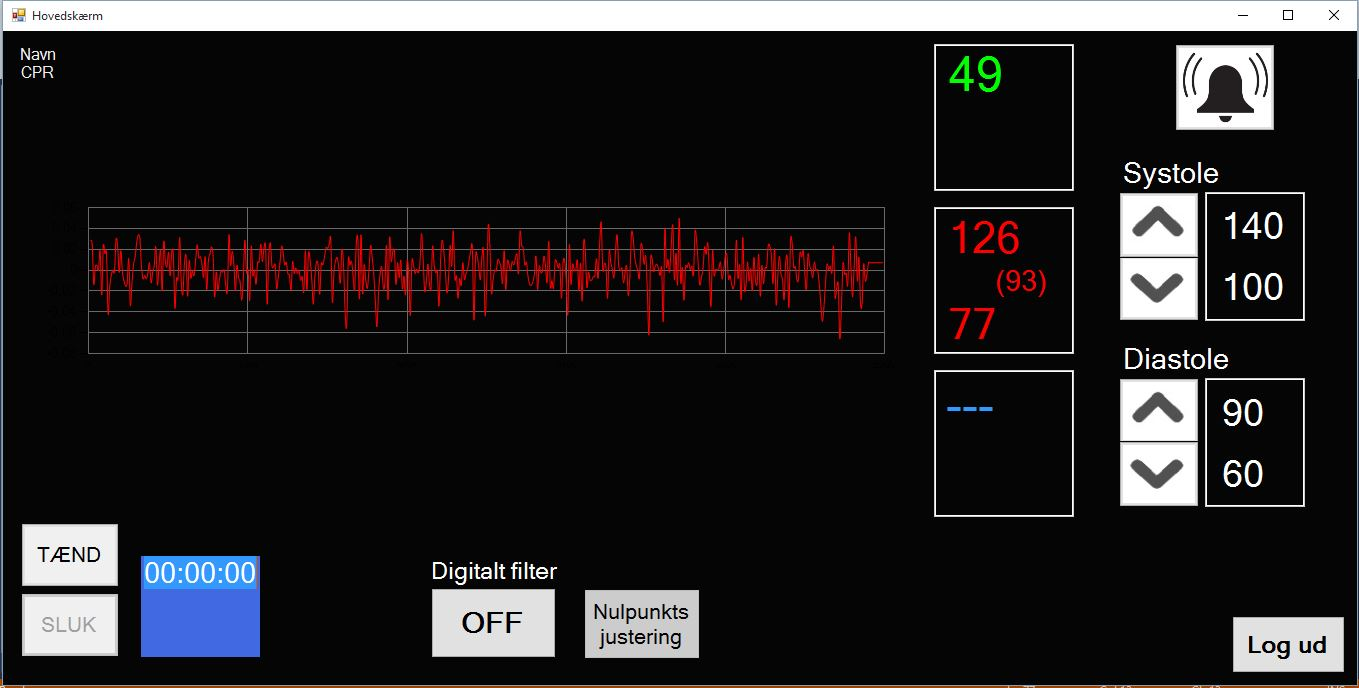
\includegraphics[width =0.8\textwidth , center]{billeder/SkitseHovedNy}
\caption{\textbf{Hovedskærmen, hvilken fungerer som blodtryksmålerens grænseflade}}
\end{figure}
\subsubsection{Domænemodel}
Først skal der klarlægges hvilke klasser som systemet skal bestå af, hvilket er det første skridt i processen. For at kunne identificere disse klasse udarbejdes en domænemodel, hvilken har sit udgangspunkt i Use cases. Det er i de konceptuelle klasser fra Use cases som indeholder den information som systemet skal holde styr på. Derfor findes de konceptuelle klasser i Use cases og disse indføres i domænemodellen som klasser. Domænemodellen opstilles derfor for at finde frem til hvad problemet er i softwaren i forhold til, hvad der skal holdes styr på.
\begin{figure}[H]
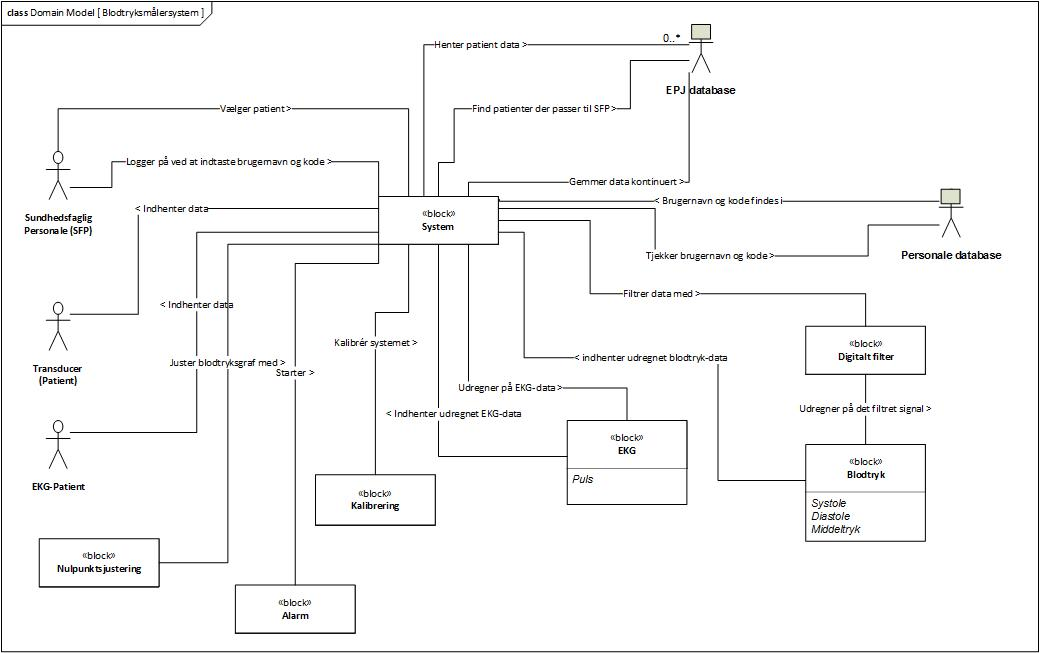
\includegraphics[width =1.0\textwidth , center]{billeder/DM}
\caption{\textbf{Domænemodel for blodtryksmålersystemet.}}
\end{figure}
Denne domænemodel viser det sundhedsfaglige personales interaktion med systemet, samt hvilke handlinger der startes af denne interaktion. Det sundhedsfaglige personale udfører en handling, der medfører, at en række processer igangsættes i systemet. Disse processer sørger for at hente data fra transduceren og EKG patient, samt sørger for at starte beregningen af puls, systolisk, diastolisk og middeltryks værdierne. Efter beregningerne viser systemet disse værdier på brugergrænsefladen, samt sørger for at disse data bliver gemt i en database.
\newpage
\subsection{Klasseidentifikation}
\subsubsection{Applikationsmodel}
Ud fra domænemodellen kan en applikationsmodel opstilles. Denne model tager afsæt i domænemodellens klasser. Dette betyder derfor at denne model således også tager udgangspunkt i alle Use cases.\\
Modellen bruges til at bestemme de interagerende klasser i blodtryksmålersystemet.\\
\begin{figure}[H]
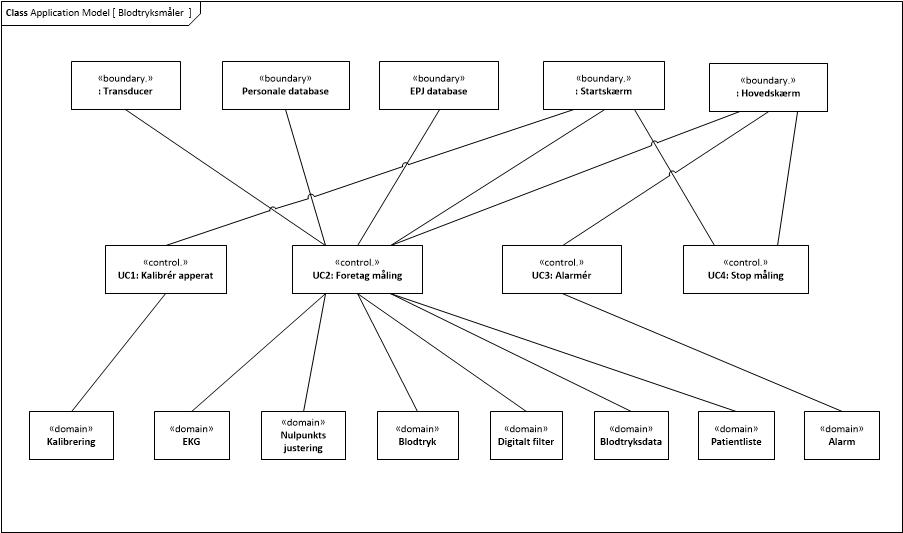
\includegraphics[width =1.0\textwidth , center]{billeder/appModel}
\caption{\textbf{Applikationsmodel for blodtryksmålersystemet.}}
\end{figure}
Ud fra denne model ses klasserne og databaserne, der skal implementeres i softwaren, samt interaktionen mellem disse. Altså hvordan klasserne taler sammen på kryds og tværs. Idet det vides at trelagsmodellen skal benyttes, kan applikationsmodellen bruges til at identificere hvor disse klasser ligger i det tilhørende lag. Databaserne vil være en boundary klasse (grænse klasse) og vil blive tilgået fra datalaget, domain klasserne (domæne klasse) er de klasser der skal ligge i logiklaget og det er disse klasser der findes fra domænemodellen og i præsentationslaget vil startskærmen og hovedskærmen, hvilke også er grænse klasser, ligge hvorfra de vil blive præsenteret for det sundhedsfaglige personale. Control klasserne (kontrol klasserne) er systemets Use cases. Grænse klasserne er de klasser der repræsentere aktørerne fra Use casene og disse aktøreres grænseflader. Domæne klasserne er de klasser hvori data bliver behandlet og bearbejdet. Kontrol klasserne er de klasser der udfører Use casene ved at interagere med grænse og domæne klasserne. \\\\
\textbf{Trelagsmodellen} \\
Trelags modellen er en software model, der gør det muligt at inddele software kodeN op i tre lag. De tre lag er præsentationslaget, logiklaget og datalaget. \\
Fordelen ved at kunne dele softwaren op på denne måde, er at man kan rette i de forskellige lag, uden at det får indflydelse i de andre lag. Man kan herved implementere nye klasser og deres funktioner, og blot henvise til dem i de andre lag. Hvert lag har deres egen funktionalitet og ansvar.\\
Præsentationslaget er det øverste lag i trelags modellen, og kan kun snakke sammen med logiklaget. I præsentationslaget må der ikke laves nogen form for beregninger, disse skal komme fra logiklaget. Med andre ord fungerer præsentationslaget, kun til at præsenter data på en brugergrænseflade, hvorfra data kan præsenteres for brugeren. Præsentationslaget er derfor også det eneste lag, som brugeren kommer til at integrerer med.\\
Logiklaget er det midterste lag, og er et bindeled mellem præsentationslaget og datalaget. I logiklaget forgår alt behandling af data fra præsentationslaget og datalaget. Det betyder at alle algoritmer skal ligge i logiklaget. \\
Datalaget er det nederste lag, og her indhentes eller gemmes data. Der kan indlæses data fra en fil, eller et måleapparat eller en database. Datalaget kan gemme data fra logiklaget i en fil eller database. \\
I trelagsmodellen kan der skabes et flydende bindeled, der kan snakke sammen med alle lagene, dette kaldes for en DTO. En DTO står for Data transfer object, og transporter objekter imellem alle lagene, og kan derved tilgås af alle lagene. \\
\\
I dette projekt er trelagsmodellen blevet opfyldt ved at der er oprettet en solution der hedder PulsMaalerSystem, under denne solution ligger der fire projekter; PulsMaalerSystem, PulsMaalerSystem.Logiklag, PulsMaalerSystem.Datalag og PulsMaalerSystem.DTOlag. Opdeling af softwarekoden i trelagsmodel kan ses på figuren nedenfor. 
\begin{figure}[H]
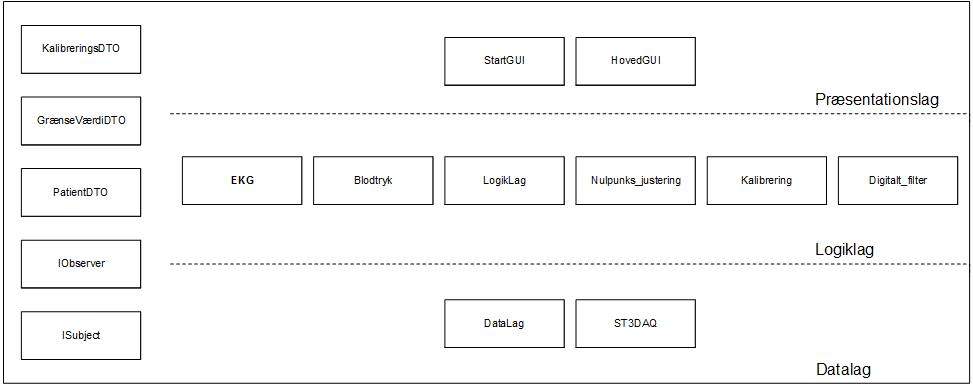
\includegraphics[width =1.0\textwidth , center]{billeder/Trelagsmodel}
\caption{\textbf{Trelagsmodellen. Her ses hvor de forskellige klasser ligger i der forskellige lag.}}
\end{figure}
Det første projekt PulsMaalerSystem fungerer som præsentationslaget og består af to Windows forms, StartGUI og HovedGUI. Begge forms sender informationer ned til logiklaget og henter data, som blodtryksværdier, og viser det på en graf. \\\\
Det andet projekt PulsMaalerSystem.Logiklag er logiklaget i projektet. I dette logiklag, er der implementeret seks klasser: Blodtryk, Kalibrering, Digitaltfilter, Nulpunkts$_{-}$justering og EKG, Logiklag.\\
Klassen Blodtryk tager sig af at udregne systolen, diastolen og middeltrykket med algoritmer ud fra blodtrykket. \\
Kalibrerings klassen sørger for at beregne kalibreringsværdien ud fra de indtastede værdier for tryk og spænding og sender denne værdi over i Logiklag klassen, hvilken kalibrér blodtrykssignalet ved at gange kalibreringsværdien på signalet.\\
Digitaltfilter klassen implementer et glidende middelværdisfilter, der sørger for at udglatte blodtrykssignalet.\\
Nulpunkts$_{-}$justering klassen sørger for at sætte signalets baseline ved 0 V. 
EKG klassen skulle have sørget for at finde R-takker og udregne pulsen. Grundet tidspres har det ikke været muligt at implementer EKG i projektet. Der er dog gjort klar til det med denne klasse. \\\\
Logiklags klassen binder alle de andre klasser sammen, ved at hente data nede fra datalaget til klasserne og sende metoderne med videre til præsentationslaget.\\
\\
Det tredje projekt PulsMaalerSystem.Datalag består af to klasser: DAQ og datalag. 
DAQ klassen sørger for at hente data op fra DAQ’en. Datalag klassen sørger for at hente informationer om patienten og personalet i databaserne; Personale database og EPJ database. Datalag klassen sørger også for at gemme blodtrykket for patienten løbende i EPJ databasen. \\
 \\
Det sidste projekt PulsMaalerSystem.DTOlag består af tre klasser: GrænseværdiDTO, IObserver, ISubject og KalibreringsDTO. GrænseværdiDTO klassen indeholder get og set metoder for grænseværdien, og sender grænseværdierne videre med en metode. IObserver kigger ned på subjectet, hvor klassen ISubject . KalibreringsDTO klassen har get og set metoder for spænding og tryk, og en metode til at sende disse videre.
\subsection{Metodeidentifikation}
\subsubsection{Sekvensdiagrammer}
Nedenfor er vist sekvensdiagrammer for systemet. Der er lavet sekvens diagrammer for alle Use case. Vores Use cases er henholdsvis Use case 1: Kalibrér apparat, Use case 2: Foretag måling, Use case 3: Alarmér og Use case 4: Stop måling. Sekvens diagrammet er et interaktionsdiagram, som viser hvorledes processerne forløber i forhold til hinanden. Ud fra sekvensdiagrammerne kan det altså ses hvornår og hvordan de forskellige dele i systemet forløber og interagerer. \\
\begin{figure}[H]
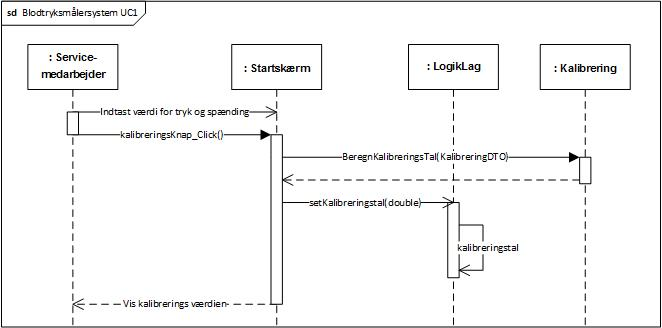
\includegraphics[width =0.8\textwidth , center]{billeder/sdUC1}
\caption{\textbf{Sekvensdiagram for blodtryksmålersystemet. Denne viser adfærden for Use case 1 }}
\end{figure}
I sekvens diagrammet for Use case 1 interagerer servicemedarbejder med blodtryksmålersystemet. Her er det servicemedarbejderen som starter kalibreringen og blodtryksmålersystemet som foretager kalibreringen igennem lagene og klassen Kalibring. Her ses det at servicemedarbejderen indtaster værdierne der aflæses for tryk og spænding, hvorefter der trykkes på knappen, hvorefter systemet foretager beregningen for kalibreringen. 
\begin{figure}[H]
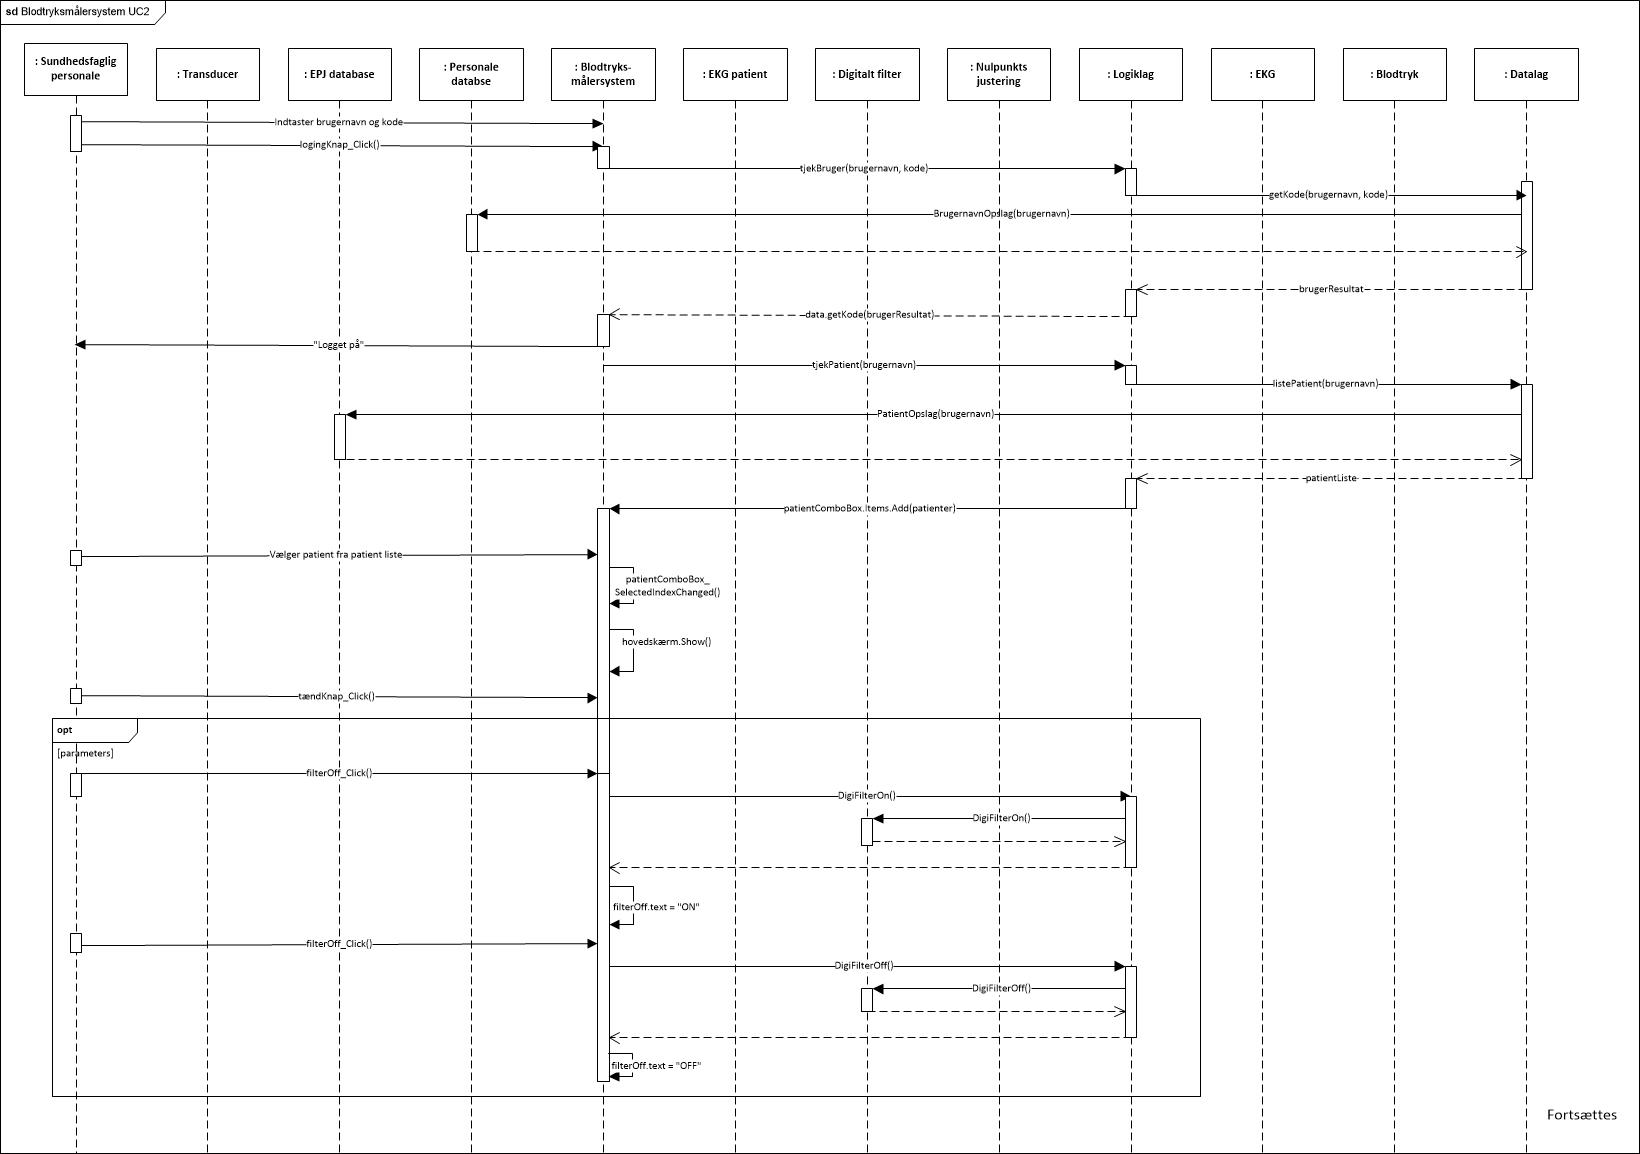
\includegraphics[width =0.8\textwidth , center]{billeder/sdUC2}
\caption{\textbf{Sekvensdiagram for blodtryksmålersystemet. Denne viser adfærden for Use case 2, del 1 af 4}}
\end{figure}
\begin{figure}[H]
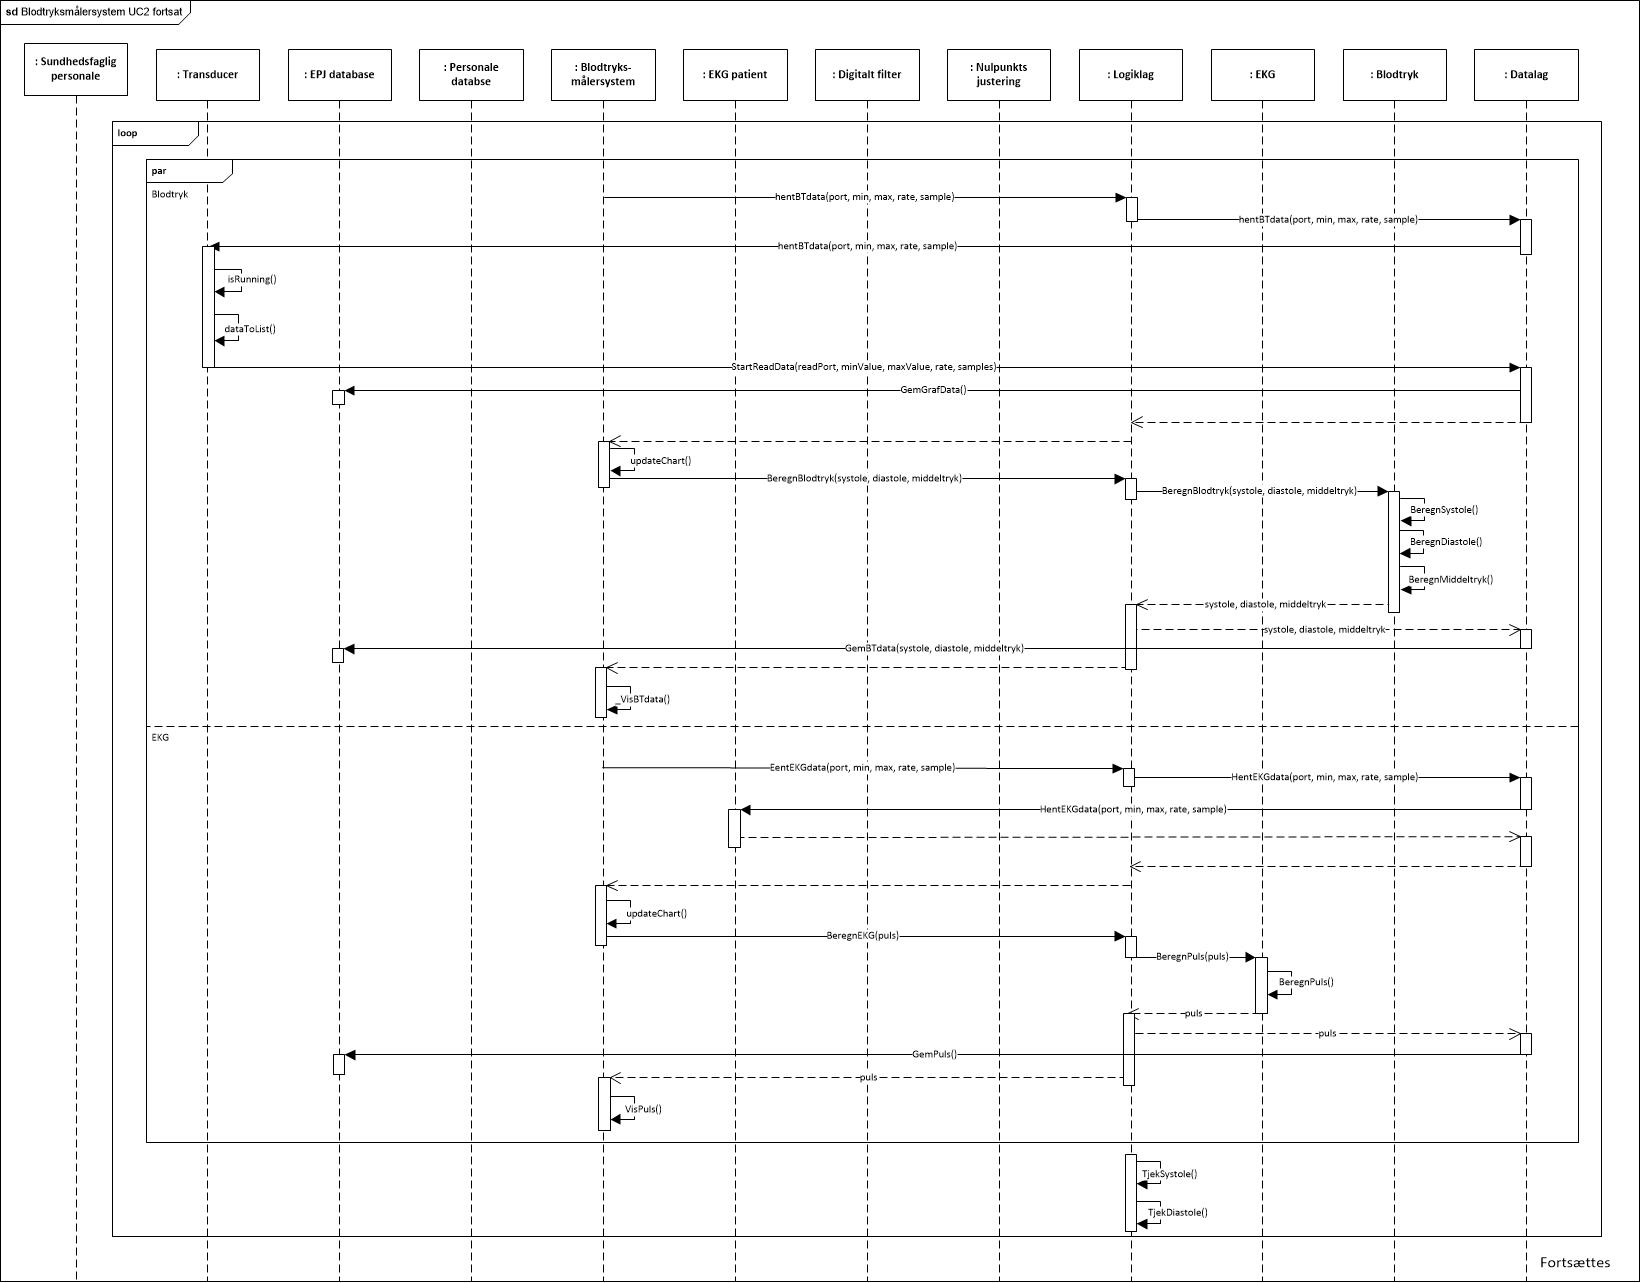
\includegraphics[width =1.0\textwidth , center]{billeder/sdUC2_2}
\caption{\textbf{Sekvensdiagram for blodtryksmålersystemet. Denne viser adfærden for Use case 2, del 2 af 4}}
\end{figure}
\begin{figure}[H]
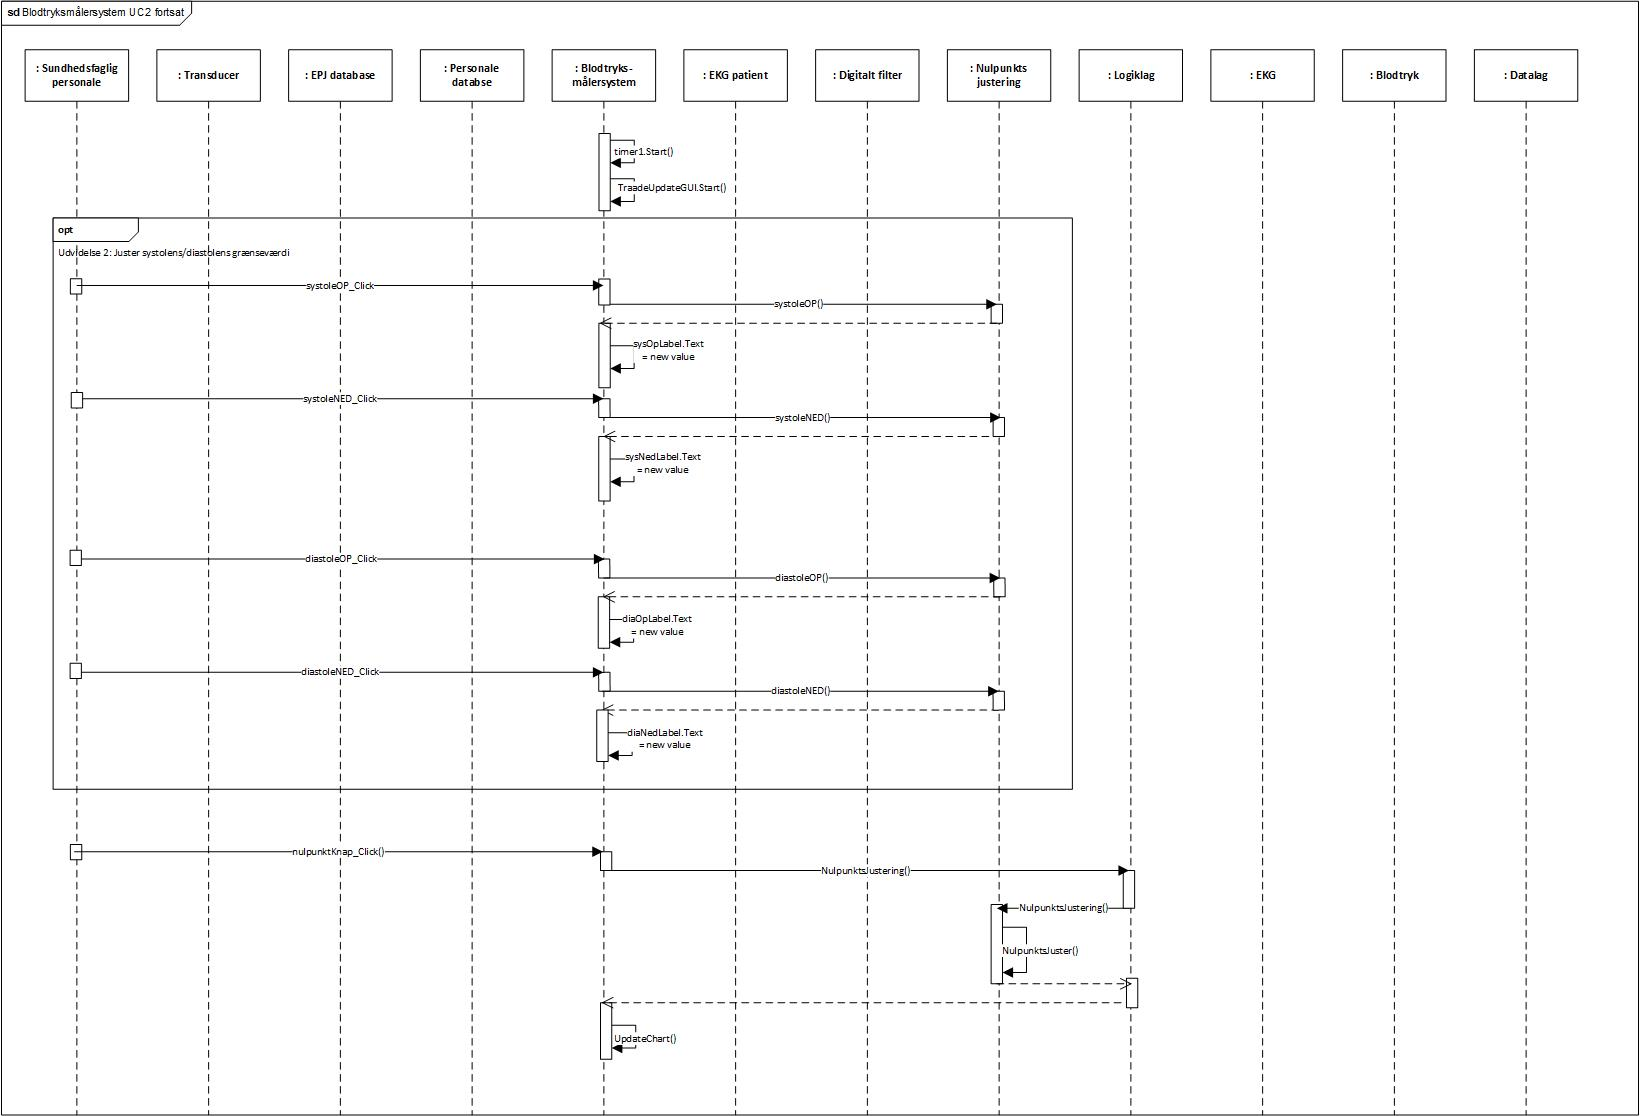
\includegraphics[width =1.0\textwidth , center]{billeder/sdUC2_3}
\caption{\textbf{Sekvensdiagram for blodtryksmålersystemet. Denne viser adfærden for Use case 2, del 3 af 4}}
\end{figure}
\begin{figure}[H]
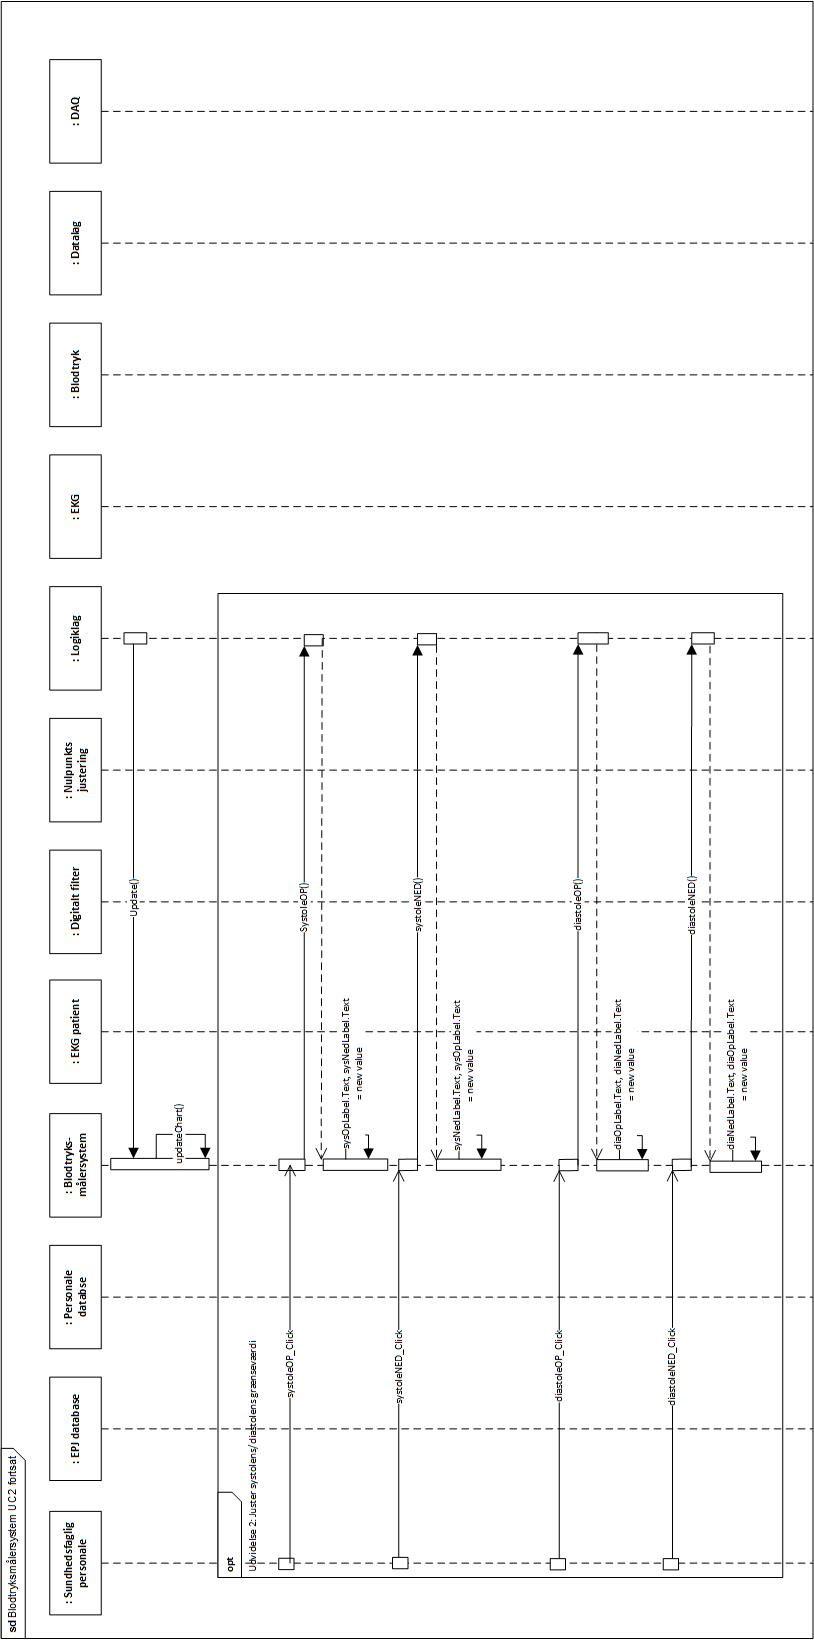
\includegraphics[width =0.7\textwidth , center]{billeder/sdUC2_4}
\caption{\textbf{Sekvensdiagram for blodtryksmålersystemet. Denne viser adfærden for Use case 2, del 4 af 4}}
\end{figure}
I sekvens diagrammet for Use case 2 ønsker det sundhedsfaglig personale at foretage måling, dette gøres ved at det sundhedsfaglig personale interagerer med blodtryksmålersystemet. For at målingen forløber, foregår den videre interaktion via blodtryksmålersystemet og de klasser, som indgår i Use casen. Transducer, EKG patient sender sine data til datalaget, EPJ database og Personale database får sine data fra datalaget. I dette sekvens diagram ses det sundhedsfaglige personales interaktion med blodtryksmålersystemet. Denne interaktion igangsætter processerne, som medfører at blodtryksmålingen forløber. Det ses også, at præsentationslaget, som er vores blodtryksmålersystem, kommunikerer med logiklaget og logiklaget kommunikerer med datalag, altså er trelagsmodellen opfyldt, idet datalaget ikke direkte kan kommunikere med præsentationslaget, men skal igennem logiklaget. \\\\
\begin{figure}[H]
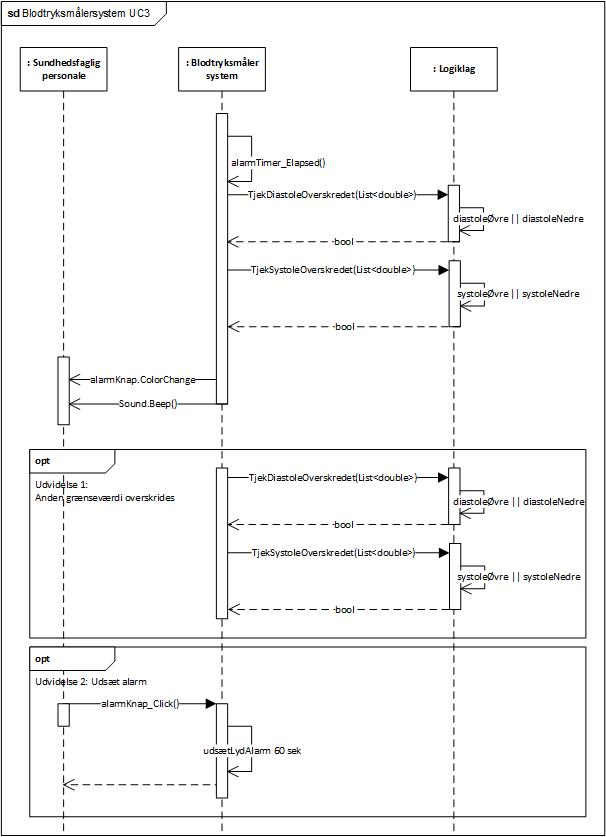
\includegraphics[width =0.8\textwidth , center]{billeder/sdUC3}
\caption{\textbf{Sekvensdiagram for blodtryksmålersystemet. Denne viser adfærden for Use case 3}}
\end{figure}
I dette sekvens diagram for Use case 3 tjekker logiklaget hvorvidt grænseværdierne for systole og diastole er overskredet. Hvis en grænseværdi overskrides starter alarmeringen. I denne Use case har det sundhedsfaglig personale mulighed for at udsætte alarmen, dette sker ved en interaktion mellem sundhedsfaglig personale og blodtryksmålersystemet.\\\\ 
\begin{figure}[H]
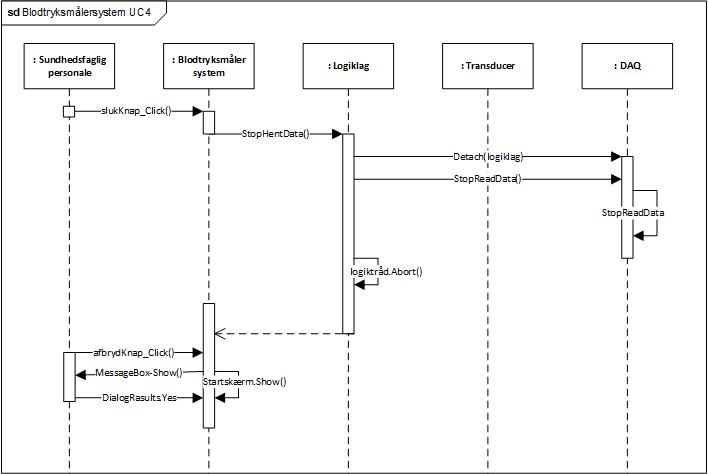
\includegraphics[width =1.0\textwidth , center]{billeder/sdUC4}
\caption{\textbf{Sekvensdiagram for blodtryksmålersystemet. Denne viser adfærden for Use case 4}}
\end{figure}
I sekvens diagrammet for Use case 4 ønsker sundhedsfaglig personale, at stoppe målingen. Dette gøres ved, at sundhedsfaglig personale interagerer med blodtryksmålersystemet i præsentationslaget. Denne interaktion medfører en videre kommunikation mellem logiklaget og datalaget, som medfører at DAQ'en ikke længere henter data fra transduceren. Når blodtryksmålingen er afsluttet kan det sundhedsfaglige personale logge ud. 
\subsubsection{Klassediagram}
Ud fra domænemodellen er der fundet ud af hvilke klasser blodtrykssystemet skal bestå af. Ud fra applikationsmodellen er samhørigheden af klasserne bestemt. Der skal være lav kobling og høj samhørighed, dette betyder at klasserne ikke må være koblet sammen på tværs i de forskellige lag. Ud fra sekvensdiagrammerne analyseres det hvilke metoder, der tilhører hver klasse.\\\\
Ud fra informationerne fra domænemodellen, applikationsmodellen og sekvensdiagrammet kan der laves et klassediagram, der indeholder attributterne og metoderne for hver klasse fra domænemodellen.
\begin{figure}[H]
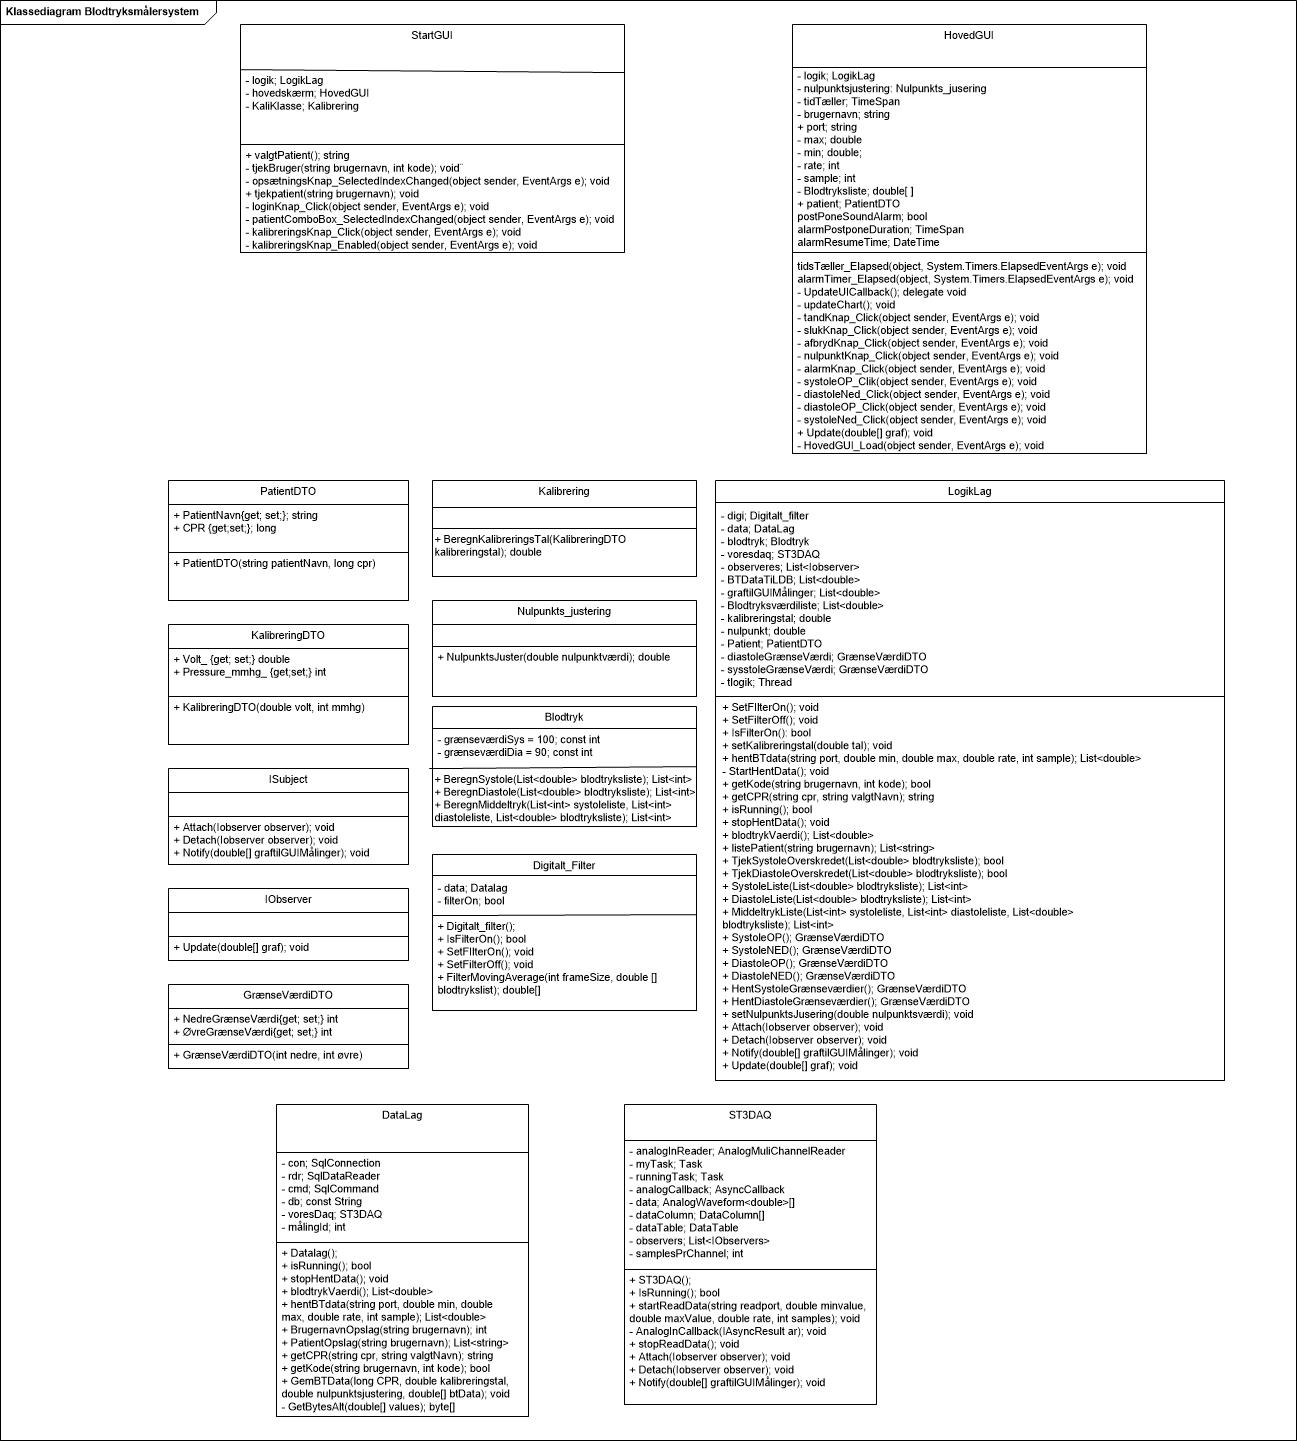
\includegraphics[width =1.0\textwidth , center]{billeder/klassediagram}
\caption{\textbf{Heraf ses klasserne med de tilhørende attributter og metoder.}}
\end{figure}
\subsubsection{Metodebeskrivelse}
Metoderne der identificeres i klassediagrammet vil her beskrives, hvor det beskrives, hvilken parameter metoden tager imod, hvilken returværdi metoden sender videre og en kort beskrivelse af metodens funktion. Event metoderne der ikke er i klassediagrammet, vil dog her ligeledes blive beskrevet. \\\\
\textbf{StartGUI}
\begin{figure}[H]
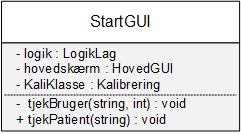
\includegraphics[width =0.4\textwidth , center]{billeder/klassediagramStart}
\caption{\textbf{Klassediagram for StartGUI.}}
\end{figure}
\begin{table}[H]
\label{tab:tabel2}
\begin{tabular}{| l | p{13cm} |}
   \hline
   \multicolumn{2}{|l|}{public StartGUI()} \\ \hline
   Parameter: & Ingen\\ \hline
   Returværdi: & Ingen \\ \hline
   Beskrivelse: & Denne metode sørger for forbindelse til LogikLag klassen og Kalibrering klassen.\\ \hline
\end{tabular}
\end{table}
\begin{table}[H]
\label{tab:tabel2}
\begin{tabular}{| l | p{13cm} |}
   \hline
   \multicolumn{2}{|l|}{private void tjekBruger(string, int)} \\ \hline
   Parameter: & string, int\\ \hline
   Returværdi: & Ingen \\ \hline
   Beskrivelse: & Metoden går ind og kalder metoden getKode() fra LogikLag klassen for at tjekke om det indtastede brugernavn og kode hører sammen.\\ \hline
\end{tabular}
\end{table}
\begin{table}[H]
\label{tab:tabel2}
\begin{tabular}{| l | p{13cm} |}
   \hline
   \multicolumn{2}{|l|}{private void opsætningKnap\_ SelectedIndexChanged(object, EventArgs)} \\ \hline
   Parameter: & object, EventArgs\\ \hline
   Returværdi: & Ingen \\ \hline
   Beskrivelse: & Metoden gør det muligt at skrive tekst i idTextBox og passwordTextBox og gør loginKnap mulig at trykke på.\\ \hline
\end{tabular}
\end{table}
\begin{table}[H]
\label{tab:tabel2}
\begin{tabular}{| l | p{13cm} |}
   \hline
   \multicolumn{2}{|l|}{public void tjekPatient(string)} \\ \hline
   Parameter: & string\\ \hline
   Returværdi: & Ingen \\ \hline
   Beskrivelse: & Denne metode går ind og kigger på hver patient i patientlisten fra LogikLag, og ser hvilke patienter som er koblet sammen med det indtastede personale brugernavn og tilføjer patienterne til listen af patienter i PatientComboBox.\\ \hline
\end{tabular}
\end{table}
\begin{table}[H]
\label{tab:tabel2}
\begin{tabular}{| l | p{13cm} |}
   \hline
   \multicolumn{2}{|l|}{private void loginKnap\_ Click(object, EventArgs)} \\ \hline
   Parameter: & object, EventArgs\\ \hline
   Returværdi: & Ingen \\ \hline
   Beskrivelse: & Metoden kalder metoden tjekBruger(), hvor det indtastede brugernavn og password sendes med. Ryder PatientComboBoxens liste. Kalder metoden tjekPatient(), som sender brugernavnet med.\\ \hline
\end{tabular}
\end{table}
\begin{table}[H]
\label{tab:tabel2}
\begin{tabular}{| l | p{13cm} |}
   \hline
   \multicolumn{2}{|l|}{private void patientComboBox\_ SelectedIndexChanged(object, EventArgs)} \\ \hline
   Parameter: & object, EventArgs\\ \hline
   Returværdi: & Ingen \\ \hline
   Beskrivelse: & Denne metode kalder PatientDTO klassen og bruger denne til at vælge patient fra patientComboBox. Sender den valgte port videre til HovedGUI. Viser HovedGUI og skjuler StartGUI.\\ \hline
\end{tabular}
\end{table}
\begin{table}[H]
\label{tab:tabel2}
\begin{tabular}{| l | p{13cm} |}
   \hline
   \multicolumn{2}{|l|}{private void kalibreringKnap\_ Click(object, EventArgs)} \\ \hline
   Parameter: & object, EventArgs\\ \hline
   Returværdi: & Ingen \\ \hline
   Beskrivelse: & Denne metode kalder KalibrerinsDTO og henter syntaksen for værdierne indtastet i Volttextbox og mmHgTextBox. Kalder metoden BeregnKalibreringsTal() i Kalibrering klassen, hvilken bruger de indtastede værdier og kalder metoden setKalibreringstal() fra LogikLag klassen, hvilken bruger den beregnede værdi. Værdien udskrives herefter på startskærmen.\\ \hline
\end{tabular}
\end{table}
\begin{table}[H]
\label{tab:tabel2}
\begin{tabular}{| l | p{13cm} |}
   \hline
   \multicolumn{2}{|l|}{private void kalibreringsKnap\_ Enabled(object, EventArgs)} \\ \hline
   Parameter: & object, EventArgs\\ \hline
   Returværdi: & Ingen \\ \hline
   Beskrivelse: & Denne metode gør kalibrerings knappen enabled, altså gør det muligt at trykke på knappen.\\ \hline
\end{tabular}
\end{table}
\textbf{HovedGUI}
\begin{figure}[H]
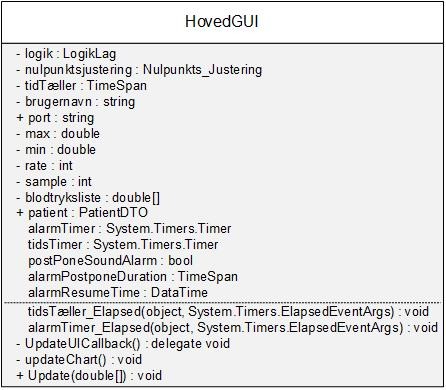
\includegraphics[width =0.7\textwidth , center]{billeder/klassediagramHoved}
\caption{\textbf{Klassediagram for HovedGUI}}
\end{figure}
\begin{table}[H]
\label{tab:tabel2}
\begin{tabular}{| l | p{13cm} |}
   \hline
   \multicolumn{2}{|l|}{public HovedGUI(string, LogikLag)} \\ \hline
   Parameter: & string, LogikLag\\ \hline
   Returværdi: & Ingen \\ \hline
   Beskrivelse: & Denne metode bruges til sætter tiden hvormed alarmen skal udsættes. Sætter det digitale filter på signalet pr. default og hvis radioButtonOFF vælges bliver det digitale filter slået fra, hvorefter det bliver muligt at slå digitalt filter til ved at vælge radioButtonON.\\ \hline
\end{tabular}
\end{table}
\begin{table}[H]
\label{tab:tabel2}
\begin{tabular}{| l | p{13cm} |}
   \hline
   \multicolumn{2}{|l|}{void tidsTæller\_ Elapsed(object, System.Timers.ElapsedEventArgs)} \\ \hline
   Parameter: & object, System.Timers.ElapsedEventArgs\\ \hline
   Returværdi: & Ingen \\ \hline
   Beskrivelse: & Metoden henter tidTæller tråden og tæller den én værdi op hvert sekund og viser værdien på HovedGUI.\\ \hline
\end{tabular}
\end{table}
\begin{table}[H]
\label{tab:tabel2}
\begin{tabular}{| l | p{13cm} |}
   \hline
   \multicolumn{2}{|l|}{void alarmTimer\_ Elapsed(object, System.Timers.ElapsedEventArgs)} \\ \hline
   Parameter: & object, System.Timers.ElapsedEventArgs\\ \hline
   Returværdi: & Ingen \\ \hline
   Beskrivelse: & Metoden kalder TjektDiastoleOverskredet() metoden fra LogikLag og kobler blodtrykslisten på denne, hvilken går ind og ser om der er en grænseværdi der er overskredet. Hvis en grænseværdi er overskredet skifter alarmKnap baggrundsbillede mellem to billeder; et rødt og et hvidt og starter en Beep.Play(). TjektSystoleOverskredet() metoden fra LogikLag kaldes og kobles til blodtrykslisten, hvilken går ind og ser om der er en grænseværdi der er overskredet. Hvis en grænseværdi er overskredet skifter alarmKnap baggrundsbillede mellem to billeder; et rødt og et hvidt, og starter en Beep.Play().\\ \hline
\end{tabular}
\end{table}
\begin{table}[H]
\label{tab:tabel2}
\begin{tabular}{| l | p{13cm} |}
   \hline
   \multicolumn{2}{|l|}{private delegate void UpdateUICallback()} \\ \hline
   Parameter: & Ingen\\ \hline
   Returværdi: & Ingen \\ \hline
   Beskrivelse: & En delegate der bliver koblet til updateChart().\\ \hline
\end{tabular}
\end{table}
\begin{table}[H]
\label{tab:tabel2}
\begin{tabular}{| l | p{13cm} |}
   \hline
   \multicolumn{2}{|l|}{private void updateChart()} \\ \hline
   Parameter: & Ingen\\ \hline
   Returværdi: & Ingen \\ \hline
   Beskrivelse: & Metoden er en tråd, hvilken går ind og ser om chart Blodtryk ligger i en anden tråd og starter tråden. Metoden går ind og sender værdier fra blodtrykslisten ind i Blodtryk chart. Henter systoliske, diastolisk og middeltryks værdier, og sender disse værdier til labels på startskærmen.\\ \hline
\end{tabular}
\end{table}
\begin{table}[H]
\label{tab:tabel2}
\begin{tabular}{| l | p{13cm} |}
   \hline
   \multicolumn{2}{|l|}{private void tandKnap\_ Click(object, EventArgs) } \\ \hline
   Parameter: & object, EventArgs\\ \hline
   Returværdi: & Ingen \\ \hline
   Beskrivelse: & Metoden kalder hentBTdata() og Attach() metoderne fra LogikLag. Kalder HentSystoleGrænseværdier() og HentDiastoleGrænseværdier() metoderne for at hente øvre og nedre grænseværdier.\\ \hline
\end{tabular}
\end{table}
\begin{table}[H]
\label{tab:tabel2}
\begin{tabular}{| l | p{13cm} |}
   \hline
   \multicolumn{2}{|l|}{private void slukKnap\_ Click(object, EventArgs) } \\ \hline
   Parameter: & object, EventArgs\\ \hline
   Returværdi: & Ingen \\ \hline
   Beskrivelse: & Denne kalder metoderne StopHentData() og Detach() fra LogikLag klassen.\\ \hline
\end{tabular}
\end{table}
\begin{table}[H]
\label{tab:tabel2}
\begin{tabular}{| l | p{13cm} |}
   \hline
   \multicolumn{2}{|l|}{private void afbrydKnap\_ Click(object, EventArgs)} \\ \hline
   Parameter: & object, EventArgs\\ \hline
   Returværdi: & Ingen \\ \hline
   Beskrivelse: & Metoden åbner en MessageBox som spørger "Er du sikker?" hvis "ja" vises StartGUI og HovedGUI skjules.\\ \hline
\end{tabular}
\end{table}
\begin{table}[H]
\label{tab:tabel2}
\begin{tabular}{| l | p{13cm} |}
   \hline
   \multicolumn{2}{|l|}{private void nulpunktKnap\_ Click(object, EventArgs)} \\ \hline
   Parameter: & object, EventArgs\\ \hline
   Returværdi: & Ingen \\ \hline
   Beskrivelse: & Metoden kalder NulpunktsJuster() fra Nulpunkts\_ justering klassen, og sender den indtastede værdi videre for at beregne værdien. setNulpunktsJustering() metoden fra LogikLag kaldes og den beregnede værdi sendes til LogikLag.\\ \hline
\end{tabular}
\end{table}
\begin{table}[H]
\label{tab:tabel2}
\begin{tabular}{| l | p{13cm} |}
   \hline
   \multicolumn{2}{|l|}{private void alarmKnap\_ Click(object, EventArgs)} \\ \hline
   Parameter: & object, EventArgs\\ \hline
   Returværdi: & Ingen \\ \hline
   Beskrivelse: & Denne metode udsætter alarmens lyd ved at kalde postPoneSoundAlarm og udsættelsens varighed sættes.\\ \hline
\end{tabular}
\end{table}
\begin{table}[H]
\label{tab:tabel2}
\begin{tabular}{| l | p{13cm} |}
   \hline
   \multicolumn{2}{|l|}{private void systoleOP\_ Click(object, EventArgs)} \\ \hline
   Parameter: & object, EventArgs\\ \hline
   Returværdi: & Ingen \\ \hline
   Beskrivelse: & Denne metode gør at de systoliske grænseværdier forøges. Metoden SystoleOP() fra LogikLag kaldes, hvorfra ØvreGrænseværdi og NedreGrænseVærdi ændres.\\ \hline
\end{tabular}
\end{table}
\begin{table}[H]
\label{tab:tabel2}
\begin{tabular}{| l | p{13cm} |}
   \hline
   \multicolumn{2}{|l|}{private void systoleNED\_ Click(object, EventArgs)} \\ \hline
   Parameter: & object, EventArgs\\ \hline
   Returværdi: & Ingen \\ \hline
   Beskrivelse: & Denne metode gør at de systoliske grænseværdier nedsænkes. Metoden SystoleNED() fra LogikLag kaldes, hvorfra ØvreGrænseværdi og NedreGrænseVærdi ændres.\\ \hline
\end{tabular}
\end{table}
\begin{table}[H]
\label{tab:tabel2}
\begin{tabular}{| l | p{13cm} |}
   \hline
   \multicolumn{2}{|l|}{private void diastoleOP\_ Click(object, EventArgs)} \\ \hline
   Parameter: & object, EventArgs\\ \hline
   Returværdi: & Ingen \\ \hline
   Beskrivelse: & Denne metode gør at de diastoliske grænseværdier forøges. Metoden DiastoleOP() fra LogikLag kaldes, hvorfra ØvreGrænseværdi og NedreGrænseVærdi ændres.\\ \hline
\end{tabular}
\end{table}
\begin{table}[H]
\label{tab:tabel2}
\begin{tabular}{| l | p{13cm} |}
   \hline
   \multicolumn{2}{|l|}{private void diastoleNED\_ Click(object, EventArgs)} \\ \hline
   Parameter: & object, EventArgs\\ \hline
   Returværdi: & Ingen \\ \hline
   Beskrivelse: &  Denne metode gør at de diastoliske grænseværdier sænkes. Metoden DiastoleNED() fra LogikLag kaldes, hvorfra ØvreGrænseværdi og NedreGrænseVærdi ændres.\\ \hline
\end{tabular}
\end{table}
\begin{table}[H]
\label{tab:tabel2}
\begin{tabular}{| l | p{13cm} |}
   \hline
   \multicolumn{2}{|l|}{public void Update(double[])} \\ \hline
   Parameter: & double[]\\ \hline
   Returværdi: & Ingen \\ \hline
   Beskrivelse: & Metoden sætter blodtrykslisten lig med et double array og kalder metoden updateChart().\\ \hline
\end{tabular}
\end{table}
\begin{table}[H]
\label{tab:tabel2}
\begin{tabular}{| l | p{13cm} |}
   \hline
   \multicolumn{2}{|l|}{private void HovedGUI\_ Load(object, EventArgs)} \\ \hline
   Parameter: & object, EventArgs\\ \hline
   Returværdi: & Ingen \\ \hline
   Beskrivelse: & Metoden sætter navn og cpr på HovedGUI ved at kalde PatientDTO, hvilken indeholder denne information.\\ \hline
\end{tabular}
\end{table}
\textbf{PatientDTO}
\begin{figure}[H]
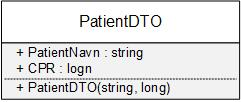
\includegraphics[width =0.4\textwidth , center]{billeder/klassediagrampatientDTO}
\caption{\textbf{Klassediagram for PatientDTO.}}
\end{figure}
\begin{table}[H]
\label{tab:tabel2}
\begin{tabular}{| l | p{13cm} |}
   \hline
   \multicolumn{2}{|l|}{public PatientDTO(string, long)} \\ \hline
   Parameter: & string, long\\ \hline
   Returværdi: & Ingen \\ \hline
   Beskrivelse: & Denne sætter syntaksen for patienten og dermed hvilke parametre denne indeholder.\\ \hline
\end{tabular}
\end{table}
\textbf{KalibreringDTO}
\begin{figure}[H]
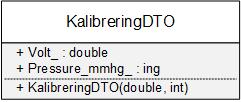
\includegraphics[width =0.4\textwidth , center]{billeder/klassediagramkalibreringDTO}
\caption{\textbf{Klassediagram for KalibreringDTO.}}
\end{figure}
\begin{table}[H]
\label{tab:tabel2}
\begin{tabular}{| l | p{13cm} |}
   \hline
   \multicolumn{2}{|l|}{public KalibreringDTO(double, int)} \\ \hline
   Parameter: & double, int\\ \hline
   Returværdi: & Ingen \\ \hline
   Beskrivelse: & Denne sætter syntaksen for kalibrering og dermed hvilke parametre der skal benyttes til kalibrering.\\ \hline
\end{tabular}
\end{table}
\textbf{ISubject}
\begin{figure}[H]
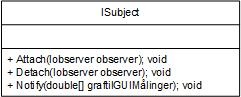
\includegraphics[width =0.4\textwidth , center]{billeder/klassediagramIsubject}
\caption{\textbf{Klassediagram for ISubject.}}
\end{figure}
\begin{table}[H]
\label{tab:tabel2}
\begin{tabular}{| l | p{13cm} |}
   \hline
   \multicolumn{2}{|l|}{void Attach(IObserver)} \\ \hline
   Parameter: & IObserver\\ \hline
   Returværdi: & Ingen \\ \hline
   Beskrivelse: & Denne metode modtager en observer.\\ \hline
\end{tabular}
\end{table}
\begin{table}[H]
\label{tab:tabel2}
\begin{tabular}{| l | p{13cm} |}
   \hline
   \multicolumn{2}{|l|}{void Detach(IObserver)} \\ \hline
   Parameter: & IObserver\\ \hline
   Returværdi: & Ingen \\ \hline
   Beskrivelse: & Denne metode modtager en observer.\\ \hline
\end{tabular}
\end{table}
\begin{table}[H]
\label{tab:tabel2}
\begin{tabular}{| l | p{13cm} |}
   \hline
   \multicolumn{2}{|l|}{void Notify(double[])} \\ \hline
   Parameter: & double[]\\ \hline
   Returværdi: & Ingen \\ \hline
   Beskrivelse: & Denne metode modtager et array med grafmålinger.\\ \hline
\end{tabular}
\end{table}
\textbf{IObserver}
\begin{figure}[H]
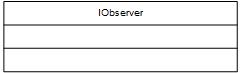
\includegraphics[width =0.4\textwidth , center]{billeder/klassediagramIobserver}
\caption{\textbf{Klassediagram for IObserver.}}
\end{figure}
\begin{table}[H]
\label{tab:tabel2}
\begin{tabular}{| l | p{13cm} |}
   \hline
   \multicolumn{2}{|l|}{void Update(double[])} \\ \hline
   Parameter: & double[]\\ \hline
   Returværdi: & Ingen \\ \hline
   Beskrivelse: & Denne metode modtager et array, hvori grafen ligger.\\ \hline
\end{tabular}
\end{table}
\textbf{GrænseVærdiDTO}
\begin{figure}[H]
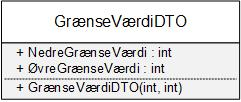
\includegraphics[width =0.4\textwidth , center]{billeder/klassediagramgransevardiDTO}
\caption{\textbf{Klassediagram for GrænseVærdiDTO.}}
\end{figure}
\begin{table}[H]
\label{tab:tabel2}
\begin{tabular}{| l | p{13cm} |}
   \hline
   \multicolumn{2}{|l|}{public GrænseVærdiDTO(int, int)} \\ \hline
   Parameter: & int, int\\ \hline
   Returværdi: & double \\ \hline
   Beskrivelse: & Metoden sætter syntaksen sådan at der skal være en øvre og nedre grænseværdi.\\ \hline
\end{tabular}
\end{table}
\textbf{Kalibrering}
\begin{figure}[H]
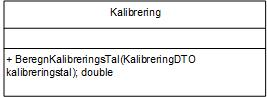
\includegraphics[width =0.4\textwidth , center]{billeder/klassediagramkalibrering}
\caption{\textbf{Klassediagram for Kalibrering.}}
\end{figure}
\begin{table}[H]
\label{tab:tabel2}
\begin{tabular}{| l | p{13cm} |}
   \hline
   \multicolumn{2}{|l|}{public double BeregnKalibreringsTal(KalibreringDTO)} \\ \hline
   Parameter: & KalibreringDTO\\ \hline
   Returværdi: & double \\ \hline
   Beskrivelse: & Denne metode beregner kalibrerings værdien ved at modtage syntaksen fra KalibreringsDTO: tryk divideret med spænding. Og returnerer denne som en double værdi.\\ \hline
\end{tabular}
\end{table}
\textbf{Nulpunkts\_ justering}
\begin{figure}[H]
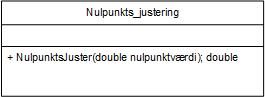
\includegraphics[width =0.4\textwidth , center]{billeder/klassediagramnulpunkt}
\caption{\textbf{Klassediagram for Nulpunkts\_ justering.}}
\end{figure}
\begin{table}[H]
\label{tab:tabel2}
\begin{tabular}{| l | p{13cm} |}
   \hline
   \multicolumn{2}{|l|}{public double NulpunktsJuster(double)} \\ \hline
   Parameter: & double\\ \hline
   Returværdi: & double \\ \hline
   Beskrivelse: & Metoden sætter nulpunktsværdien, ved at trække den indtastede værdi fra nul og returnere denne værdi som en double.\\ \hline
\end{tabular}
\end{table}
\textbf{Blodtryk}
\begin{figure}[H]
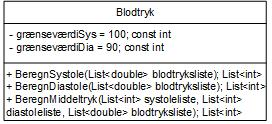
\includegraphics[width =0.4\textwidth , center]{billeder/klassediagramblodtryk}
\caption{\textbf{Klassediagram for Blodtryk.}}
\end{figure}
\begin{table}[H]
\label{tab:tabel2}
\begin{tabular}{| l | p{13cm} |}
   \hline
   \multicolumn{2}{|l|}{public List<int> BeregnSystole(List<double>)} \\ \hline
   Parameter: & List<double>\\ \hline
   Returværdi: & List<int> \\ \hline
   Beskrivelse: & Metoden går ind og kigger på samtlige værdier i blodtryksliste. Metoden ser om værdien er over en sat baseline, hvis den er det, går metoden ind og ser om den næste værdi er højere, når værdien bliver lavere igen tilføjer metoden den højeste værdi til listen toppunkter og returnerer denne liste. \\ \hline
\end{tabular}
\end{table}
\begin{table}[H]
\label{tab:tabel2}
\begin{tabular}{| l | p{13cm} |}
   \hline
   \multicolumn{2}{|l|}{public List<int> BeregnDiastole(List<double>)} \\ \hline
   Parameter: & List<double>\\ \hline
   Returværdi: & List<int> \\ \hline
   Beskrivelse: & Metoden går ind og kigger på samtlige værdier i blodtryksliste. Metoden ser om værdien er under en sat baseline, hvis den er det, går metoden ind og ser om den næste værdi er lavere, når værdien bliver højere igen tilføjer metoden den laveste værdi til listen minimumspunkter og returnerer denne liste. \\ \hline
\end{tabular}
\end{table}
\begin{table}[H]
\label{tab:tabel2}
\begin{tabular}{| l | p{13cm} |}
   \hline
   \multicolumn{2}{|l|}{public List<int> BeregnMiddeltryk(List<int>, List<int>, List<double>)} \\ \hline
   Parameter: & List<int>, List<int>, List<double>\\ \hline
   Returværdi: & List<int> \\ \hline
   Beskrivelse: & Metoden går ind og kigger på samtlige værdier i diastolelisten og systolelisten. Metoden tager  her en værdi for diastole og en værdi for systole og beregner middeltryk ved formlen: $\dfrac{2}{3}diastole+\dfrac{1}{3}systole$. Tilføjer værdien til en middeltrykliste og returnerer denne. \\ \hline
\end{tabular}
\end{table}
\textbf{Digitalt\_ filter}
\begin{figure}[H]
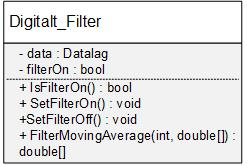
\includegraphics[width =0.4\textwidth , center]{billeder/klassediagramdigi}
\caption{\textbf{Klassediagram for Digitalt\_ Filter.}}
\end{figure}
\begin{table}[H]
\label{tab:tabel2}
\begin{tabular}{| l | p{13cm} |}
   \hline
   \multicolumn{2}{|l|}{public Digitalt\_ filter()} \\ \hline
   Parameter: & Ingen\\ \hline
   Returværdi: & Ingen \\ \hline
   Beskrivelse: & Denne sætter boolean filterOn lig med true. \\ \hline
\end{tabular}
\end{table}
\begin{table}[H]
\label{tab:tabel2}
\begin{tabular}{| l | p{13cm} |}
   \hline
   \multicolumn{2}{|l|}{public bool IsFilterOn()} \\ \hline
   Parameter: & Ingen\\ \hline
   Returværdi: & bool\\ \hline
   Beskrivelse: & Metoden returnerer filterOn\\ \hline
\end{tabular}
\end{table}
\begin{table}[H]
\label{tab:tabel2}
\begin{tabular}{| l | p{13cm} |}
   \hline
   \multicolumn{2}{|l|}{public bool SetFilterOn()} \\ \hline
   Parameter: & Ingen\\ \hline
   Returværdi: & Ingen\\ \hline
   Beskrivelse: & Metoden sætter filterOn lig true.\\ \hline
\end{tabular}
\end{table}
\begin{table}[H]
\label{tab:tabel2}
\begin{tabular}{| l | p{13cm} |}
   \hline
   \multicolumn{2}{|l|}{public bool SetFilterOff()} \\ \hline
   Parameter: & Ingen\\ \hline
   Returværdi: & Ingen\\ \hline
   Beskrivelse: & Metoden sætter filterOn lig false.\\ \hline
\end{tabular}
\end{table}
\begin{table}[H]
\label{tab:tabel2}
\begin{tabular}{| l | p{13cm} |}
   \hline
   \multicolumn{2}{|l|}{public double[] FilterMovingAverage(int, double[])} \\ \hline
   Parameter: & int, double[]\\ \hline
   Returværdi: & double[]\\ \hline
   Beskrivelse: & Metoden gør sådan at blodtryklisten kører igennem en ramme, hvor gennemsnittet beregnes af rammens indhold og rammen rykker én plads efter beregningen, sådan at beregningen sker glidende på blodtrykslisten. Metoden returnerer det beregnede gennemsnit i et double array. \\ \hline
\end{tabular}
\end{table}
\textbf{LogikLag}
\begin{figure}[H]
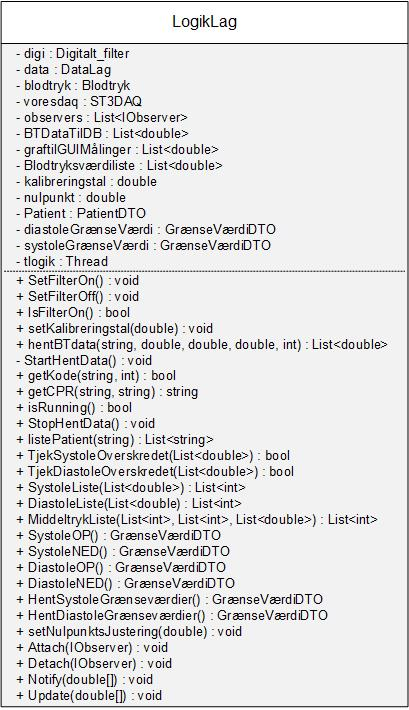
\includegraphics[width =0.7\textwidth , center]{billeder/klassediagramLogik}
\caption{\textbf{Klassediagram for LogikLag.}}
\end{figure}
\begin{table}[H]
\label{tab:tabel2}
\begin{tabular}{| l | p{13cm} |}
   \hline
   \multicolumn{2}{|l|}{public void SetFilterOn()} \\ \hline
   Parameter: & Ingen\\ \hline
   Returværdi: & Ingen\\ \hline
   Beskrivelse: & Denne metode kalder Digitalt\_ filter klassens metode SetFilterOn() \\ \hline
\end{tabular}
\end{table}
\begin{table}[H]
\label{tab:tabel2}
\begin{tabular}{| l | p{13cm} |}
   \hline
   \multicolumn{2}{|l|}{public void SetFilterOff()} \\ \hline
   Parameter: & Ingen\\ \hline
   Returværdi: & Ingen\\ \hline
   Beskrivelse: & Denne metode kalder Digitalt\_ filter klassens metode SetFilterOff() \\ \hline
\end{tabular}
\end{table}
\begin{table}[H]
\label{tab:tabel2}
\begin{tabular}{| l | p{13cm} |}
   \hline
   \multicolumn{2}{|l|}{public bool IsFilterOn()} \\ \hline
   Parameter: & Ingen\\ \hline
   Returværdi: & bool\\ \hline
   Beskrivelse: & Denne metode returnerer Digitalt\_ filter metoden IsFilterOn() \\ \hline
\end{tabular}
\end{table}
\begin{table}[H]
\label{tab:tabel2}
\begin{tabular}{| l | p{13cm} |}
   \hline
   \multicolumn{2}{|l|}{public void setKalibreringstal(double)} \\ \hline
   Parameter: & double\\ \hline
   Returværdi: & Ingen\\ \hline
   Beskrivelse: & Metoden sætter kalibreringstallet til et double tal. \\ \hline
\end{tabular}
\end{table}
\begin{table}[H]
\label{tab:tabel2}
\begin{tabular}{| l | p{13cm} |}
   \hline
   \multicolumn{2}{|l|}{public void hentBTdata(string, double, double, double, int, PatientDTO)} \\ \hline
   Parameter: & string, double, double, double, int, PatientDTO\\ \hline
   Returværdi: & Ingen\\ \hline
   Beskrivelse: & Metoden kalder ST3DAQ metoden startReadData(). Implementere og starter tråden af typen StartHentData i logiklaget.\\ \hline
\end{tabular}
\end{table}
\begin{table}[H]
\label{tab:tabel2}
\begin{tabular}{| l | p{13cm} |}
   \hline
   \multicolumn{2}{|l|}{Private void StartHentData()} \\ \hline
   Parameter: & Ingen\\ \hline
   Returværdi: & Ingen\\ \hline
   Beskrivelse: & Metoden laver en kø-metode med 500 pladser. Kalder Attach() metoden fra ST3DAQ. Så længde metoden isRunning gælder, og der kommer værdier ind, sendes der værdier ind i køen indtil der er 500 objekter i denne, hvor efter der sendes et objekt ud inden der sendes et nyt ind. Inden objekterne tilføjes til køen, bliver nulpunktværdien lagt til, og kalibreringsværdien bliver ganget på hvert tal i Blodtryksværdilisten. Herefter kaldes tælleren sådan at der kun tages hvert tiende tal i Blodtryksværdilisten. Digitalt\_ filter metoden IsFilterOn() kaldes, hvilket tjekker om filteret er slået til, hvis filteret er det kaldes metoden Digitalt\_ filter FilterMovingAverage() hvilket gør at værdierne i kømetoden bliver filtreret. Notify metoden kalds til sidst for at sende arrayet med den behandlede data op til HovedGUI\\ \hline
\end{tabular}
\end{table}
\begin{table}[H]
\label{tab:tabel2}
\begin{tabular}{| l | p{13cm} |}
   \hline
   \multicolumn{2}{|l|}{public bool getKode(string, int)} \\ \hline
   Parameter: & string, int\\ \hline
   Returværdi: & bool\\ \hline
   Beskrivelse: & Metoden returnerer koden, hvor denne er lig med koden, som hentes med brugernavn parameteren, fra metoden getKode fra DataLag.  \\ \hline
\end{tabular}
\end{table}
\begin{table}[H]
\label{tab:tabel2}
\begin{tabular}{| l | p{13cm} |}
   \hline
   \multicolumn{2}{|l|}{public string getCPR(string, string)} \\ \hline
   Parameter: & string, sting\\ \hline
   Returværdi: & string\\ \hline
   Beskrivelse: & Metoden returnerer cpr. \\ \hline
\end{tabular}
\end{table}
\begin{table}[H]
\label{tab:tabel2}
\begin{tabular}{| l | p{13cm} |}
   \hline
   \multicolumn{2}{|l|}{public bool isRunning()} \\ \hline
   Parameter: & Ingen\\ \hline
   Returværdi: & bool\\ \hline
   Beskrivelse: & Metoden returnerer ST3DAQ klassens metode IsRunning(). \\ \hline
\end{tabular}
\end{table}
\begin{table}[H]
\label{tab:tabel2}
\begin{tabular}{| l | p{13cm} |}
   \hline
   \multicolumn{2}{|l|}{public void StopHentData()} \\ \hline
   Parameter: & Ingen\\ \hline
   Returværdi: & Ingen\\ \hline
   Beskrivelse: & Metoden kalder ST3DAQ klassens metoder Detach() og StopReadData(). Metoden stopper tråden der startes i hentBTdata(). \\ \hline
\end{tabular}
\end{table}
\begin{table}[H]
\label{tab:tabel2}
\begin{tabular}{| l | p{13cm} |}
   \hline
   \multicolumn{2}{|l|}{public List<PatientDTO> listePatient(string)} \\ \hline
   Parameter: & string\\ \hline
   Returværdi: & List<PatientDTO>\\ \hline
   Beskrivelse: & Metoden returnerer metoden PatientOpslag() fra DataLag, hvilken har syntaksen fra PatientDTO.\\ \hline
\end{tabular}
\end{table}
\begin{table}[H]
\label{tab:tabel2}
\begin{tabular}{| l | p{13cm} |}
   \hline
   \multicolumn{2}{|l|}{public bool TjekSystoleOverskredet(List<double>)} \\ \hline
   Parameter: & List<double>\\ \hline
   Returværdi: & bool\\ \hline
   Beskrivelse: & Metoden henter systoleværdierne ved at kalder BeregnSystole() metoden fra Blodtryk. Metoden tjekker om systole værdien er over den øvre grænseværdi eller under den nedre grænseværdi og hvis én af værdierne har en højere/lavere værdi er grænseværdien overskredet. Metoden returnerer resultatet. \\ \hline
\end{tabular}
\end{table}
\begin{table}[H]
\label{tab:tabel2}
\begin{tabular}{| l | p{13cm} |}
   \hline
   \multicolumn{2}{|l|}{public bool TjekDiastoleOverskredet(List<double>)} \\ \hline
   Parameter: & List<double>\\ \hline
   Returværdi: & bool\\ \hline
   Beskrivelse: & Metoden henter diastoleværdierne ved at kalder BeregnDiastole() metoden fra Blodtryk. Metoden tjekker om diastole værdien er over den øvre grænseværdi eller under den nedre grænseværdi og hvis én af værdierne har en højere/lavere værdi er grænseværdien overskredet. Metoden returnerer resultatet. \\ \hline
\end{tabular}
\end{table}
\begin{table}[H]
\label{tab:tabel2}
\begin{tabular}{| l | p{13cm} |}
   \hline
   \multicolumn{2}{|l|}{public List<int> SystoleListe(List<double>)} \\ \hline
   Parameter: & List<double>\\ \hline
   Returværdi: & List<int>\\ \hline
   Beskrivelse: &  Metoden returnerer en liste med systoler ved at koble blodtrykslisten sammen med metoden BeregnSystole() fra Blodtryk.\\ \hline
\end{tabular}
\end{table}
\begin{table}[H]
\label{tab:tabel2}
\begin{tabular}{| l | p{13cm} |}
   \hline
   \multicolumn{2}{|l|}{public List<int> DiastoleListe(List<double>)} \\ \hline
   Parameter: & List<double>\\ \hline
   Returværdi: & List<int>\\ \hline
   Beskrivelse: &  Metoden returnerer en liste med diastoler ved at koble metoden BeregnDiastole() fra Blodtryk sammen med blodtrykslisten.\\ \hline
\end{tabular}
\end{table}
\begin{table}[H]
\label{tab:tabel2}
\begin{tabular}{| l | p{13cm} |}
   \hline
   \multicolumn{2}{|l|}{public List<int> Middeltrykliste(List<int>, List<int>, List<double>)} \\ \hline
   Parameter: & List<int>, List<int>, List<double>\\ \hline
   Returværdi: & List<int>\\ \hline
   Beskrivelse: &  Metoden returnerer en liste med middeltryksværdier ved at kalde metoden BeregnMiddeltryk() fra Blodtryk og koble denne sammen med systolelisten, diastolelisten og blodtrykslisten.\\ \hline
\end{tabular}
\end{table}
\begin{table}[H]
\label{tab:tabel2}
\begin{tabular}{| l | p{13cm} |}
   \hline
   \multicolumn{2}{|l|}{public GrænseVærdiDTO SystoleOP()} \\ \hline
   Parameter: & Ingen \\ \hline
   Returværdi: & GrænseVærdiDTO\\ \hline
   Beskrivelse: & Metoden kalder den nedre og øvre grænseværdi og gør begge grænseværdier én større. Metoden returnerer de nye grænseværdier med syntaksen fra GrænseVærdiDTO.\\ \hline
\end{tabular}
\end{table}
\begin{table}[H]
\label{tab:tabel2}
\begin{tabular}{| l | p{13cm} |}
   \hline
   \multicolumn{2}{|l|}{public GrænseVærdiDTO SystoleNED()} \\ \hline
   Parameter: & Ingen \\ \hline
   Returværdi: & GrænseVærdiDTO\\ \hline
   Beskrivelse: & Metoden kalder den nedre og øvre grænseværdi og gør begge grænseværdier én mindre. Metoden returnerer de nye grænseværdier med syntaksen fra GrænseVærdiDTO.\\ \hline
\end{tabular}
\end{table}
\begin{table}[H]
\label{tab:tabel2}
\begin{tabular}{| l | p{13cm} |}
   \hline
   \multicolumn{2}{|l|}{public GrænseVærdiDTO DiastoleOP()} \\ \hline
   Parameter: & Ingen \\ \hline
   Returværdi: & GrænseVærdiDTO\\ \hline
   Beskrivelse: & Metoden kalder den nedre og øvre grænseværdi og gør begge grænseværdier én større. Metoden returnerer de nye grænseværdier med syntaksen fra GrænseVærdiDTO.\\ \hline
\end{tabular}
\end{table}
\begin{table}[H]
\label{tab:tabel2}
\begin{tabular}{| l | p{13cm} |}
   \hline
   \multicolumn{2}{|l|}{public GrænseVærdiDTO DiastoleNED()} \\ \hline
   Parameter: & Ingen \\ \hline
   Returværdi: & GrænseVærdiDTO\\ \hline
   Beskrivelse: & Metoden kalder den nedre og øvre grænseværdi og gør begge grænseværdier én mindre. Metoden returnerer de nye grænseværdier med syntaksen fra GrænseVærdiDTO.\\ \hline
\end{tabular}
\end{table}
\begin{table}[H]
\label{tab:tabel2}
\begin{tabular}{| l | p{13cm} |}
   \hline
   \multicolumn{2}{|l|}{public GrænseVærdiDTO HentSystoleGrænseværdier()} \\ \hline
   Parameter: & Ingen \\ \hline
   Returværdi: & GrænseVærdiDTO\\ \hline
   Beskrivelse: & Metoden returnerer grænseværdierne for systole.\\ \hline
\end{tabular}
\end{table}
\begin{table}[H]
\label{tab:tabel2}
\begin{tabular}{| l | p{13cm} |}
   \hline
   \multicolumn{2}{|l|}{public GrænseVærdiDTO HentDiastoleGrænseværdier()} \\ \hline
   Parameter: & Ingen \\ \hline
   Returværdi: & GrænseVærdiDTO\\ \hline
   Beskrivelse: & Metoden returnerer grænseværdierne for diastole.\\ \hline
\end{tabular}
\end{table}
\begin{table}[H]
\label{tab:tabel2}
\begin{tabular}{| l | p{13cm} |}
   \hline
   \multicolumn{2}{|l|}{public void setNulpunktsJustering(double)} \\ \hline
   Parameter: & double \\ \hline
   Returværdi: & Ingen\\ \hline
   Beskrivelse: & Metoden sætter nulpunktværdien til et double tal.\\ \hline
\end{tabular}
\end{table}
\begin{table}[H]
\label{tab:tabel2}
\begin{tabular}{| l | p{13cm} |}
   \hline
   \multicolumn{2}{|l|}{public void Attach(IObserver)} \\ \hline
   Parameter: & IObserver \\ \hline
   Returværdi: & Ingen\\ \hline
   Beskrivelse: & Metoden tilføjer en observer til IObserver.\\ \hline
\end{tabular}
\end{table}
\begin{table}[H]
\label{tab:tabel2}
\begin{tabular}{| l | p{13cm} |}
   \hline
   \multicolumn{2}{|l|}{public void Detach(IObserver)} \\ \hline
   Parameter: & IObserver \\ \hline
   Returværdi: & Ingen\\ \hline
   Beskrivelse: & Metoden fjerner en observer fra IObserver.\\ \hline
\end{tabular}
\end{table}
\begin{table}[H]
\label{tab:tabel2}
\begin{tabular}{| l | p{13cm} |}
   \hline
   \multicolumn{2}{|l|}{public void Notify(double[])} \\ \hline
   Parameter: & double[] \\ \hline
   Returværdi: & Ingen\\ \hline
   Beskrivelse: & Metoden kigger på hver observer i IObserver og kalder her metoden Update().\\ \hline
\end{tabular}
\end{table}
\begin{table}[H]
\label{tab:tabel2}
\begin{tabular}{| l | p{13cm} |}
   \hline
   \multicolumn{2}{|l|}{public void Update(double[])} \\ \hline
   Parameter: & double[] \\ \hline
   Returværdi: & Ingen\\ \hline
   Beskrivelse: & Metoden tilføjer et double array til blodtryksværdiliste og BTDataTilDB der bruges til at gemme data. Denne metode kalder metoden GemBTData() fra DataLag og gemmer når BTDataTilDB listen indeholder 1000 elementer og ryder derefter listen for denne kan tage 1000 nye elementer. \\ \hline
\end{tabular}
\end{table}
\textbf{DataLag}
\begin{figure}[H]
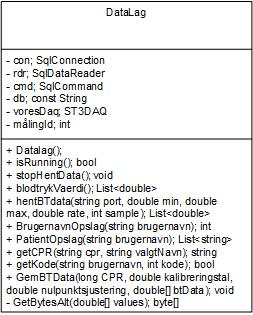
\includegraphics[width =0.4\textwidth , center]{billeder/klassediagramdata}
\caption{\textbf{Klassediagram for DataLag.}}
\end{figure}
\begin{table}[H]
\label{tab:tabel2}
\begin{tabular}{| l | p{13cm} |}
   \hline
   \multicolumn{2}{|l|}{public DataLag()} \\ \hline
   Parameter: & Ingen\\ \hline
   Returværdi: & Ingen\\ \hline
   Beskrivelse: & Metoden skaber forbindelse til de to databaser der benyttes og laver forbindelse til ST3DAQ.\\ \hline
\end{tabular}
\end{table}
\begin{table}[H]
\label{tab:tabel2}
\begin{tabular}{| l | p{13cm} |}
   \hline
   \multicolumn{2}{|l|}{public int BrugernavnOpslag(string)} \\ \hline
   Parameter: & string \\ \hline
   Returværdi: & int\\ \hline
   Beskrivelse: & Metoden kalder en metode der åbner Personale databasen, og oprettet en SQL kommando, hvor der hentes alt fra Personale tabellen hvor brugernavn er lig med brugernavn parameteren. En metode til at udføre kommando kaldes. Metoden undersøger om brugernavnet passer, lukker databasen og returnerer svaret. \\ \hline
\end{tabular}
\end{table}
\begin{table}[H]
\label{tab:tabel2}
\begin{tabular}{| l | p{13cm} |}
   \hline
   \multicolumn{2}{|l|}{public List<PatientDTO> PatientOpslag(string)} \\ \hline
   Parameter: & string \\ \hline
   Returværdi: & List<PatientDTO>\\ \hline
   Beskrivelse: & Metoden laver en patientliste der indholder syntaksen fra PatientDTO. Kalder en metode der åbner Patient databasen, og oprettet en SQL kommando, hvor der hentes alt fra Patient tabellen hvor den sundhedsfaglige er lig med brugernavn parameteren. En metode til at udføre kommando kaldes. Metoden undersøger om der findes en patient med tilkobling til den sundhedsfaglige og tilføjer CPR og Navn til patientlisten. Metoden lukker databasen og returnerer patientlisten. \\ \hline
\end{tabular}
\end{table}
\begin{table}[H]
\label{tab:tabel2}
\begin{tabular}{| l | p{13cm} |}
   \hline
   \multicolumn{2}{|l|}{public int getCPR(string)} \\ \hline
   Parameter: & string \\ \hline
   Returværdi: & int\\ \hline
   Beskrivelse: & Metoden kalder en metode der åbner Patient databasen, og oprettet en SQL kommando, hvor CPR hentes fra Patient tabellen hvor Navn er lig med patient parameteren. En metode til at udføre kommandoen kaldes. Metoden henter CPR for patienten, lukker databasen og returnerer CPR. \\ \hline
\end{tabular}
\end{table}
\begin{table}[H]
\label{tab:tabel2}
\begin{tabular}{| l | p{13cm} |}
   \hline
   \multicolumn{2}{|l|}{public int getKode(string)} \\ \hline
   Parameter: & string \\ \hline
   Returværdi: & int\\ \hline
   Beskrivelse: & Metoden kalder en metode der åbner Patient databasen, og oprettet en SQL kommando, hvor Adgangskode hentes fra Personale tabellen hvor Brugernavn er lig med brugernavn parameteren. En metode til at udføre kommandoen kaldes. Metoden henter koden for den sundhedsfaglige, lukker databasen og returnerer koden. \\ \hline
\end{tabular}
\end{table}
\begin{table}[H]
\label{tab:tabel2}
\begin{tabular}{| l | p{13cm} |}
   \hline
   \multicolumn{2}{|l|}{public void GemBTData(long, double, double, double[])} \\ \hline
   Parameter: & long, double, double, double[] \\ \hline
   Returværdi: & Ingen\\ \hline
   Beskrivelse: & Metoden kalder en metode der åbner Patient databasen, og oprettet en SQL kommando, hvor CPR, Dato, KalibreringsTalog NulpunktsjusteringsTal indsættes i Målinger tabellen. En metode til at udføre kommandoen kaldes. Metoden lukker databasen. Metoden kalder en metode der åbner Patient databasen igen, og oprettet en SQL kommando, hvor BTdata og MålingId indsættes i BTdata tabellen. En metode til at udføre kommandoen kaldes. Metoden lukker databasen.  \\ \hline
\end{tabular}
\end{table}
\begin{table}[H]
\label{tab:tabel2}
\begin{tabular}{| l | p{13cm} |}
   \hline
   \multicolumn{2}{|l|}{ private byte[] GetBytesAlt(double[])} \\ \hline
   Parameter: & double[] \\ \hline
   Returværdi: & byte[]\\ \hline
   Beskrivelse: & Metoden konverterer double array til byte array. Bruges til at gemme data i SQL-database. Metoden bruges i GemBTData() metoden. \\ \hline
\end{tabular}
\end{table}

\textbf{ST3DAQ}
\begin{figure}[H]
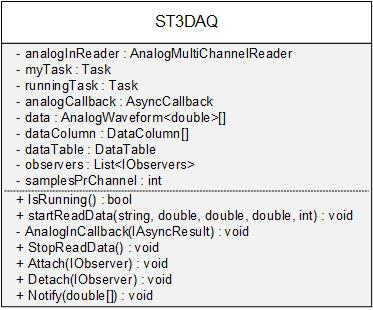
\includegraphics[width =0.6\textwidth , center]{billeder/klassediagramdaq}
\caption{\textbf{Klassediagram for ST3DAQ.}}
\end{figure}
\begin{table}[H]
\label{tab:tabel2}
\begin{tabular}{| l | p{13cm} |}
   \hline
   \multicolumn{2}{|l|}{public ST3DAQ()} \\ \hline
   Parameter: & Ingen \\ \hline
   Returværdi: & Ingen\\ \hline
   Beskrivelse: &  Metoden henter en liste af observers fra IObservers.\\ \hline
\end{tabular}
\end{table}
\begin{table}[H]
\label{tab:tabel2}
\begin{tabular}{| l | p{13cm} |}
   \hline
   \multicolumn{2}{|l|}{public bool IsRunning()} \\ \hline
   Parameter: & Ingen \\ \hline
   Returværdi: & bool\\ \hline
   Beskrivelse: & Metoden tjekker om tasken kører. Hvis den kører returnerer den true ellers returnerer denne false. \\ \hline
\end{tabular}
\end{table}
\begin{table}[H]
\label{tab:tabel2}
\begin{tabular}{| l | p{13cm} |}
   \hline
   \multicolumn{2}{|l|}{public void startReadData(string, double, double, double, int)} \\ \hline
   Parameter: & string, double, double, double, int \\ \hline
   Returværdi: & Ingen\\ \hline
   Beskrivelse: & Denne metode starter for en ny opgave, hvilken henter data fra NI-DAQ. Data hentes ved at bruge metoderne koblet til National Instruments ved at kalde Task(). \\ \hline
\end{tabular}
\end{table}
\begin{table}[H]
\label{tab:tabel2}
\begin{tabular}{| l | p{13cm} |}
   \hline
   \multicolumn{2}{|l|}{private void AnalogInCallback(IAsyncResult)} \\ \hline
   Parameter: & IAsyncResult \\ \hline
   Returværdi: & Ingen\\ \hline
   Beskrivelse: & Metoden er en delegate, der tjekker om NI-DAQ henter data og laver et asynkront kald. Tilføjer alle data fra NI-DAQ i et array. Dette array bliver notificeret med metoden Notify(). Efter stoppes opgaven startet i startReadData().\\ \hline
\end{tabular}
\end{table}
\begin{table}[H]
\label{tab:tabel2}
\begin{tabular}{| l | p{13cm} |}
   \hline
   \multicolumn{2}{|l|}{public void Attach(IObserver)} \\ \hline
   Parameter: & IObserver \\ \hline
   Returværdi: & Ingen\\ \hline
   Beskrivelse: & Metoden tilføjer en observer til IObserver.\\ \hline
\end{tabular}
\end{table}
\begin{table}[H]
\label{tab:tabel2}
\begin{tabular}{| l | p{13cm} |}
   \hline
   \multicolumn{2}{|l|}{public void Detach(IObserver)} \\ \hline
   Parameter: & IObserver \\ \hline
   Returværdi: & Ingen\\ \hline
   Beskrivelse: & Metoden fjerner en observer fra IObserver.\\ \hline
\end{tabular}
\end{table}
\begin{table}[H]
\label{tab:tabel2}
\begin{tabular}{| l | p{13cm} |}
   \hline
   \multicolumn{2}{|l|}{public void Notify(double[])} \\ \hline
   Parameter: & double[] \\ \hline
   Returværdi: & Ingen\\ \hline
   Beskrivelse: & Metoden kigger på hver observer i IObserver og kalder her metoden Update().\\ \hline
\end{tabular}
\end{table}

\subsection{Implementering}
\subsubsection{Kalibrering}
Kalibreringen er blevet implementeret sådan at der indtastes en værdi for trykket som vandsøjlen leverer i mmHg og en værdi for spændingen i volt, hvilken kan aflæses fra waveforms eller måles vha. et multimeter. Disse to værdier bliver herefter sendt ned i software klassen Kalibrering, hvor en kalibreringsværdi/omsætningsværdi kan udregnes ved formlen:
\begin{align}
X\left[\dfrac{mmHg}{V}\right]=\dfrac{pressure \left[mmHg\right]}{voltage \left[V\right]}
\end{align}
Den værdi der her udregnes benyttes herefter til at omregne den spænding i volt, der indsendes i systemet, til tryk i mmHg. 
\begin{align}
voltage \left[V\right]\cdot X\left[\dfrac{mmHg}{V}\right] = pressure \left[mmHg\right]
\end{align}
Hermed ganges kalibreringsværdien på samtlige værdier i den liste af data der kommer fra DAQ'en (Blodtryksværdiliste). 
\subsubsection{Nulpunktsjustering}
Nulpunktsjusteringen foregår ved at transduceren er tilsluttet og måler det atmosfæriske tryk, denne værdi skal herefter trækkes fra samtlige værdier for blodtrykket fra DAQ'en. Denne værdi skal derfor trækkes fra inden kalibreringsværdien ganges på. Måden hvormed nulpunktsjusteringen foregår på, er ved at transduceren er tilsluttet og vha. waveforms kan det atmosfæriske tryk aflæses, denne værdi aflæses som en spænding. Denne værdi indtastes på hovedskærmen, hvorefter nulpunktsjusteringen kan startes. Systemet går herefter ind i klassen Nulpunkts$_{-}$justering, hvor følgende formel bruges til at beregne den værdi der skal benyttes videre:
\begin{align}
V_{zero} \left[V\right]=V_{read}\left[V\right]-pressure \left[V\right] 
\end{align}
Det er denne værdi der herefter bliver kalibreret, for derefter at kunne blive vist som en graf for blodtrykket i mmHg.
\subsubsection{Digitalt filter}
Det digitale filter der er blevet implementeret i projektet er af typen et glidende middelværdi filter. I et glidende middelværdi filter, lægges der et vindue oven på ens talværdi, i dette vindue tager man gennemsnittet af alle værdien. \cite{digifilter} Vinduet er her betegnelsen for et bestemt tidsinterval. \\
I projektet er der valgt længden ti på vinduet, det betyder at for hver tiende tal i vores blodtrykliste, bliver der udregnet gennemsnittet af. Herefter rykker vinduet sig til højre og udregner for de næste ti tal i blodtrykslisten. Blodtrykslisten er listen af blodtryksværdier, der bliver indlæst af DAQ’en. 
\begin{figure}[H]
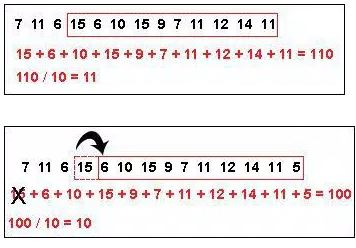
\includegraphics[width =0.5\textwidth , center]{billeder/RammeDigi}
\caption{\textbf{Digital filter ramme. Denne viser hvordan rammen bestemmer gennemsnittet og rykker én hver gang.}}
\end{figure}
Længden af vinduet på ti er valgt, da der bliver vist ti tal fra blodtrykslisten på en graf på brugergrænsefladen. 
Glidende middelværdifilter kan beskrives med formlen:
\begin{align}
y\left[n\right] = \dfrac{1}{M}\cdot \sum_{k=0}^{M}x\left[n-k\right],\\ b_{k}=\dfrac{1}{M}
\end{align}
$M$ er de forgående samples for signalet, $n$ er de nuværende værdier af blodtrykket og $k$ er koefficienterne. 
Filteret udglatter signalets høje peak værdier, da filteret er et lavpasfilter.
\subsubsection{Beregning af systolisk, diastolisk og middeltryks værdi}
Algoritmerne for udregning af systole, diastole og middeltryk er alle implementeret i klassen Blodtryk. \\
Systolen er toppunkterne i blodtryksdataene. Dette kræver dog at man skrive en kort algoritme, så man kan holde styr på hvor langt man er kommet i blodtrykslisten og hvor mange systole værdier der er fundet.\\
Der er valgt at lave en baseline, som er den grænseværdi der skal overskrides, inden man tjekker efter for toppunkter.  Grænseværdien baseline er sat til 100, da den normale værdi for systolen ligger omkring 120 mmHg.  \\\\
Algoritmen BeregnSystole starter med en for lykke, hvor man har en tæller "i", der starter fra nul og tæller op til længden af blodtrykslisten. Inden i for lykken er der en if lykke, som tjekker om indeks "i" i blodtrykslisten er større end den baseline der er sat. Hvis indeks "i" i blodtrykslisten er større end baseline, vides der at grafen er på vej opad. Herved sættes der en ny basline, som er lig med værdien for indeks "i" i blodtrykslisten.  Der bliver lagt én til værdien baselineoverskredet.\\\\ 
Hvis indeks "i" i blodtrykslisten er mindre end baseline og baslineoverskredet er større end 1, vides der at grafen for blodtrykslisten falder. Når blodtrykslisten falder vides der at den forgående indeks i blodtrykslisten er topppunktet. Der bliver gemt det forgående indeks i blodtrykslisen i en liste der hedder toppunkter. Listen af toppunkterlisten med værdier, er derfor listen af systole værdierne. Baselineoverskredet sættes lig nul, samtidig med at baselinen sættes lig default værdien, der var 100 mmHg. Algoritmen returnerer en liste af toppunkter.\\\\
Diastolen er minimumspunkterne i blodtrykslisten. For at finde minimumspunkterne i listen, er der implementeret en algoritme kaldet BeregnDiastole, som finder minimumspunkterne og gemmer dem i en liste.\\
Algoritmen er opbygget på samme måde som med BeregnSystole, med en lille ændring af at algoritmen skal finde minimumspunkter i stedet for toppunkter.\\
Der sættes en baseline værdi, der er den værdi der skal tjekkes for om indekset i blodtrykslisten er mindre ind. Default værdien for baseline er sat 90 mmHg, for at være sikker på at indekset i blodtrykslisten finder sig neden for denne værdi.\\\\
 Algoritmen BeregnDiastole starter med en for lykke, hvor man har en tæller "i", der starter fra nul og tæller op til længden af blodtrykslisten. Inden i for lykken er der en if lykke, som tjekker om indeks "i" i blodtrykslisten er mindre end den baseline der sat. Hvis indeks "i" i blodtrykslisten er mindre end baseline, vides der at grafen er på vej opad. Herved sættes der en ny basline, som er lig med værdien for indeks "i" i blodtrykslisten.  Der bliver lagt én til værdien baselineoverskredet. \\\\
Hvis indeks "i" i blodtrykslisten er større end baseline og baslineoverskredet er større end 1, vides der at grafen for blodtrykslisten stiger. Når blodtrykslisten stiger vides der at den forgående indeks i blodtrykslisten er minimumspunkter. Der bliver gemt det forgående indeks i blodtrykslisen i en liste der hedder minimumspunkter. Listen af minimumspunkter med værdier, er derfor listen af diastole værdierne. Baselineoverskredet sættes lig nul, samtidig med at baselinen sættes lig default værdien, der var 90 mmHg.\\\\
Algortimen til udregning af middeltrykket, udregner middeltrykket med \cite{blodtrykwiki} formlen:
\begin{align}
Middeltryk = \dfrac{2}{3}\cdot Diastoliske tryk + \dfrac{1}{3} \cdot Systoliske tryk
\end{align}
Algoritmen middeltryk starter med en for lykke med en tæller "i", der starter fra nul og tæller op til og med længden af blodtrykslisten. Inde i for lykken udregnes ligningen for middeltrykket for indeks "i", med systolelisten for indeks "i" og diastolelisten for indeks "i". Det udregnede middeltryk gemmes i en liste kaldet middeltrykliste. 
\subsubsection{EKG-signal}
Implementeringen af EKG-signalet er i dette projekt ikke sket. Dette er ikke implementeret, da der ikke har været tid til dette. Hvis der dog havde været tid til dette, ville Semesterprojekt 2: EKG diagnostik, været blevet benyttet til at få grundstrukturen til at se hvordan denne implementering skulle foregå.
\subsubsection{Iltmætning}
Desuden blev iltsaturation ikke implementeret. Dermed bliver iltmætningen ikke vist for patienten. Dette er ikke blevet implementeret på grund af flere faktorer: Der er ikke nok tid, der er ikke den fornødne viden til at få implementeret dette og der haves ikke de nødvendige materialer.
\subsubsection{Observer mønster med PUSH}
Observer møsteret benyttes i dette projekt for at sørge for at data bliver sendt igennem alle lagene på en fornuftig og kontinuer måde.\\
Subject kan være en abstrakt klasse eller et interface, der har tre metoder; en metode der tilknytter en observer, som gerne vil modtage opdateringer, en metode til at fjerne observeren og en notify metode. Notify metoden giver informationen til observeren om ændringer.\\
Observer er et interface, som skal implementeres af alle de klasser, hvilke skal have besked, når der sker en ændring. Der bruges en observer, når der skal ændres i et objekt og det ikke vides hvor mange objekter der skal ændres i. Observer modtager besked om ændringer fra subjectet, dette kan ske enten ved PUSH eller PULL mønsteret. \\\\
PULL fungerer ved at subjectet giver besked til observeren om at der er ændringer. Observeren sender besked til subjectet om at modtage ændringerne. Subjectet sender herefter ændringen til observeren.
PUSH fungerer sådan at subjectet giver besked til observeren, om at der er sket en ændring, samtidig med at den sender dataene med op. Data bliver altså i PUSH mønster skubbet op, hvor data i PULL trækkes op. I dette projekt er det PUSH mønsteret der er valgt at arbejde med.\\ 
\\
I projektet er der valgt at implementere to interfaces; IObserver og ISubject.Disse to interfaces er implementeret i PUSH mønsteret, der sørger for at der hele tiden sendes data op, når der er en ny opdatering. \\
\\
ISubject består af tre metoder. En metode til Attache en eller flere observer. En anden metode til at fjerne en eller flere observer. Den tredje metode Notify informerer observerne om, at der er sket en opdatering. Notify metoden sender en liste med data op til obseveren, det ses heraf at PUSH mønsteret benyttes.\\
I projektet er der valgt at skubbe data fra datalaget til logiklaget, og derefter fra logiklaget til præsentationslaget. \\ 
Der bliver derfor i projektet implementeret to ISubjects og to IObservers. Datalaget fungerer som subject for logiklaget, som er observer til datalaget. Så hver gang der bliver læste tal ind af DAQ’en, skubber datalaget disse data videre til logiklaget. \\
Logiklaget er subject for præsentationslaget. Præsentationslaget er observer for logiklaget, og får derfor skubbet data op fra logiklaget.
\subsubsection{Queue}
For at være sikker på at den data, der er blevet nulpunktsjusteret og kalibreret bliver sendt korrekt op til præsentationslaget bliver der benyttet en kø metode: Queue Class \cite{queue}. Dette er en klasse der er indbygget i Visual Studio. Denne klasse har to metoder, hvilke benyttes til at sende data ind i den rigtige ende, hvorefter data fjernes fra den anden ende når køen er fuld. \\Disse to metoder er Enqueue(object) og Dequeue(). Enqueue(object) er metoden, hvilken tilføjer et object til køen. Dette object er data fra Blodtryksværdiliste. Metoden ligger i en for-løkke, sådan at data kommer ind sådan som de indlæses fra DAQ'en. \\\\
Dequeue() er metoden, som fjerne et object fra den anden ende, og tager den første værdi i rækken og fjerner. Denne metode ligger ligeledes i for-løkken, hvorunder der er if/else metoder. Dette sørger for at køen er fuld inden der bliver fjernet en værdi fra den anden ende og dermed sørger for at de to metoder følges ad.
\subsubsection{Konfiguration}
Man har i programmet valgt at benytte sig af en konfigurationsfil, denne fil holder oplysninger i XML-format omkring opsætningen af softwaren. Det er blevet besluttet at holde det i konfigurationsfilen, for nemmere at kunne ændre indstillinger løbende under test og udvikling. Ligeledes er det valgt at skrive kalibreringskoefficienten ind i konfigurationsfilen for at simulere at en tekniker kan kalibrere programmet og ændre tallet. Det er også blevet besluttet at ligge SQL-"connectionstrings" ud i config, normalt ville man i et program som dette have en test-database og en produktions-database. Af samme grund er det vigtigt der er ét centralt sted hvor dette kan ændres.
\subsubsection{Databaser}
\begin{figure}[H]
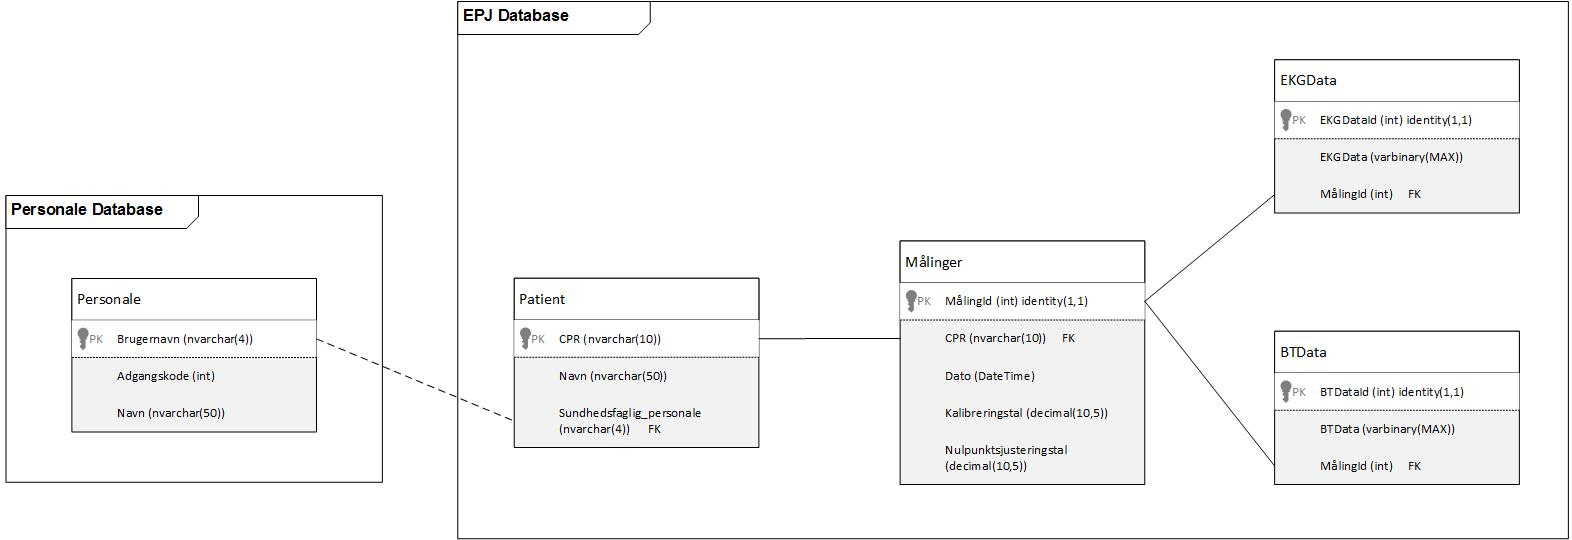
\includegraphics[width =1.0\textwidth , center]{billeder/databaser}
\caption{\textbf{Databaserne; Personale database og EPJ database. Her ses sammenhængen mellem tabellerne i databasen, og hvilken data der er under hver tabel.}}
\end{figure}
Dette afsnit vil beskrive opbygningen af databaser og tabellerne. Da der er valgt at tage udgangspunkt i et brugsscenarie, afspejler datamodelleringen i databasen dette scenarie. Det er vigtigt at bemærke at der er en regulær opdeling af databaser og skemaer, realiseret som beskrevet nedenfor.
\\\\
\textbf{Personale database}\\
Personale databasen bliver brugt til at tilgå data for personalet. Her er der tale om brugernavn og password. Disse data er lagt i databasen på forhånd, så det er altså en login-database.\\ 
\textbf{Database-adresse:} webhotel10.F15ST2ITS2201404669.db\_ owner
\\\\
\textbf{EPJ database}\\
EPJ databasen bliver brugt til at tilgå data for patienten. Her tænkes på CPR/Navn. Ligeledes gemmes der i denne database målinger, samt metadata for at kvalificere disse data. Der kunne udvides med mange flere metadata, specielt i forhold til afsnittet om fremtidigt arbejde "Datawarehouse". Det bør bemærkes der i databasen er gjort klar til EKG-data, selvom det ikke er implementeret. Patient-tabellen modsvarer vores version af en EPJ-database, hvor BTData-tabellen repræsenterer målingerne foretaget af vores system.\\
\textbf{Database-adresse:} webhotel10.F15ST2ITS2201405838.db\_ owner
\\\\
\textbf{Opdeling}\\
Man ville normalt have en "Foreign Key"-constraint fra Patient-tabellen til Personal-tabellen. Men da de befinder sig i to forskellige skemaer, der simulerer to forskellige databaser, så er det ikke en fornuftig løsning. Man ville i stedet benytte sig af en "trigger" der kan håndtere en evt. Fejl. Det er ikke en korrekt løsning og vi har valgt ikke at implementere den, men det er bedre end at "satse" på data stemmer overens. Man ville sandsynligvis løse problemet i software, eller hvis begge tabeller findes i samme skema. \\
Et eksempel på sådan en trigger vil se sådan her ud;
\begin{figure}[H]
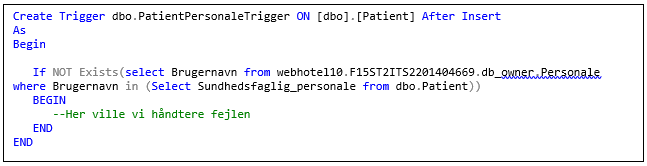
\includegraphics[width =0.5\textwidth , center]{billeder/database_kode}
\caption{\textbf{Eksempel på en trigger.}}
\end{figure}
\subsection{Unittest}
Det er blevet besluttet at lave unittest på softwaren. Ved unit-test forstås at man tester hver enkelt komponent i koden, i objektorienteret kode vil det sige metoderne. Man sikrer sig at metoderne returnerer det man forventer. En unit test bør foregå løbende lige så frit som koden bliver udviklet, så kan man fokusere på de del-elementer som ikke virker efter hensigten. \\\\
I dette projekt valgte man at lave unit test efter sidste iteration af koden, da de sidste versioner af softwaren ændrede sig meget, så alle unittests skulle laves forfra. Grundlaget for mange metoder ændrede sig løbende. Disse unit-tests blev lavet i koden ved at sætte breakpoints og følge metoden til ende og evaluere på hvorvidt metoden opførte sig efter hensigten. Unit-tests er blevet foretaget i koden, man har skrevet kommentarer til de metoder der er blevet testet.
\subsubsection{Code review}
Desuden er der blevet foretaget omfattende code-review, som en er en gennemgang af koden og de metodikker og formatering der er benyttet. Code-review er blevet foretaget af en person fra hardware-holdet. Gennemgangen har resulteret i nogle formateringsændringer i koden, ligeledes er kodesegmenter der ikke bliver brugt kommenteret ud.
\subsubsection{Databaser og test}
Databasetest er blevet foretaget i det tilgængelige testmiljø, det vil sige serverne er placeret på IHA og der kræves VPN for at kunne tilgå dem. Der er i projektet benyttet to databaser for at simulere separat personale og EPJ databaser. \\\\
\textbf{Personale database}\\
Bliver brugt til at tilgå data for personalet. Her er der tale om brugernavn og password. Disse data er lagt i databasen på forhånd.\\
Database-adresse: webhotel10.F15ST2ITS2201404669.db\_ owner
\begin{figure}[H]
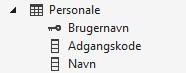
\includegraphics[width =0.2\textwidth , center]{billeder/database_p_tabel}
\caption{\textbf{Personale database med kolonner}}
\end{figure}
\textbf{EPJ database}\\
Bliver brugt til at tilgå data for patienten. Her tænkes på CPR/Navn. Ligeledes gemmes der i denne database målinger, samt metadata for at kvalificere disse data. Der kunne udvides med mange flere metadata, specielt i forhold til afsnittet om fremtidigt arbejde "Datawarehouse". Det bør bemærkes der i databasen er gjort klar til EKG-data, selvom det ikke er implementeret.\\
Database-adresse: webhotel10.F15ST2ITS2201405838.db\_ owner
\begin{figure}[H]
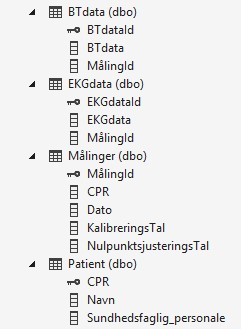
\includegraphics[width =0.2\textwidth , center]{billeder/database_e_tabel}
\caption{\textbf{EPJ database med kolonner.}}
\end{figure}
\textbf{Test}\\
Testen af databaser er foregået løbende. Da softwareløsningen gemmer data kontinuert, så kan man altså tjekke om data bliver gemt ved at tjekke tabellernes indhold løbende. 
\begin{figure}[H]
\includegraphics[width =0.5\textwidth , center]{billeder/database_data_gem}
\caption{\textbf{Udsnit af data gemt i Målinger.}}
\end{figure}
\begin{figure}[H]
\includegraphics[width =0.3\textwidth , center]{billeder/database_bt_gem}
\caption{\textbf{Udsnit af data gemt i BTData.}}
\end{figure}
\section{Integrationstest}
\chapter{Accepttest}
\section{Indledning}
Accepttestene skal vise om kravene der er opstillet for blodtryksmålersystemet i kravspecifikationen lever op til de standarder der er sat op for at produktet aktivt kan indgå i en hverdag på sygehusene.\\
Accepttestene er er opfølgning af kravspecifikationen, hvilket sikre at alle krav er overholdt og dermed opnået.\\\\
Når der i feltet Godkendt er skrevet initialer for den der har udført testen, samt datoen for testens udførelse, betyder det at testen er godkendt.  \\
Igennem Arkitektur og design er systemet blevet identificeret og specificeret, sadan at vides hvilke dele systemet består af og hvordan dette skal præsenteres på user interfaces.
\section{Accepttest for funktionelle krav}
\subsection{Opstilling}
Billede indsættes - haves ikke endnu
\\
\begin{table}[H]
\caption{Accepttest for Use case 1}\label{tab:tabel8}
\begin{tabular}{|>{\raggedright\arraybackslash}p{2.5cm}| >{\raggedright\arraybackslash}p{2.9cm} | >{\raggedright\arraybackslash}p{2.9cm} | >{\raggedright\arraybackslash}p{2.9cm} | >{\raggedright\arraybackslash}p{2.8cm} |}
   \hline
   \textbf{Use case 1: Kalibrer apparat} &\textbf{Test}& \textbf{Prækondition} & \textbf{Forventet resultat} & \textbf{Godkendt/ kommentar}\\ \hline
   Normalforløb: & Vælg et målepunkt på vandsøjlen. Indtast den aflæste værdi for spændingen, og aflæs trykket fra vandsøjlens skema for målepunktet. & Blodtryksmåler-systemet er tændt, tilsluttet og startet, og tilsluttet kalibreringsudstyret. & Service-medarbejder foretager kalibrering. Værdierne indtastes korrekt. & \\\hline
   & Tryk på "Kalibrering" & Blodtryksmåler-systemet er tændt og tilsluttet, og tilsluttet kalibreringsudstyret og værdierne indtastet. & Systemet beregner kalibreringsværdien og kalibrerer systemet, resultatet af beregningen vises på startskærmen & \\\hline
\end{tabular}
\end{table}

\begin{table}[H]
\caption{Accepttest for Use case 1}\label{tab:tabel8}
\begin{tabular}{|>{\raggedright\arraybackslash}p{2.5cm}| >{\raggedright\arraybackslash}p{2.9cm} | >{\raggedright\arraybackslash}p{2.9cm} | >{\raggedright\arraybackslash}p{2.9cm} | >{\raggedright\arraybackslash}p{2.8cm} |}
   \hline
   \textbf{Use case 1: Kalibrer apparat} &\textbf{Test}& \textbf{Prækondition} & \textbf{Forventet resultat} & \textbf{Godkendt/ kommentar}\\ \hline
 Undtagelse 1:Undlad kalibrering & Undlad kalibrering og fortsæt til Use case 2. & Blodtryksmåler-systemet er tilsluttet og tændt & Kalibrerings-værdien hentes, fra den forrige måling, fra EPJ databasen. & \\\hline
\end{tabular}
\end{table}
Det forudsættes for de følgende Use cases (Use case 2, 3 og 4) at systemet er tilsluttet korrekt, porten til NI-DAQ er bestemt, at der er en VPN-forbindelse til "ASE IHA VPN", desuden skal der være en forbindelse til $"webhotel10.F15ST2ITS2201404669.db_{-}owner"$(Personaledatabasen) og $"webhotel10.F15ST2ITS2201405838.db_{-}owner"$ (EPJ database). Desuden skal blodtryksmålersystemet være tilsluttet In vitro maskinen.
\begin{table}[H]
\caption{Accepttest for Use case 2}\label{tab:tabel9}
\begin{tabular}{|>{\raggedright\arraybackslash}p{2.5cm}| >{\raggedright\arraybackslash}p{2.9cm} | >{\raggedright\arraybackslash}p{2.9cm} | >{\raggedright\arraybackslash}p{2.9cm} | >{\raggedright\arraybackslash}p{2.8cm} |}
   \hline
   \textbf{Use case 2: Foretag måling} &\textbf{Test}& \textbf{Prækondition} & \textbf{Forventet resultat} & \textbf{Godkendt/ kommentar}\\ \hline
   Normalforløb:& Indtast brugernavn "anpe" og kode "1234" & Port valgt. Der er VPN-forbindelse. & Korrekt indtastning fuldendt & \\\hline
   &Tryk "Log ind" & Port valgt. VPN, Personale database. & Besked: "Logget på" og den sundhedsfaglige er dermed logget på &\\\hline
   &Tryk på patient dropdown på startskærm & En sundhedsfaglig er logget på & Liste med patienter kommer frem  & \\\hline
   & Vælg patienten "Arne Jensen" & Den sundhedsfaglige er logget på & Nyt vindue kommer frem: Hovedskærmen &\\\hline
   & Indsend atmosfærisk tryk igennem transduceren, indstil værdien efter grafen. & Patient valgt og blodtryksmålersystemet (transduceren) er tilsluttet & Nulpunkts-justerings værdien indtastes &\\\hline
   & Tryk på "Nulpunkts justering" & Værdien er indtastet & Systemet starter nulpunkts justeringen og tilpasser grafen. &\\\hline
   & Tryk på "Tænd"& Systemet er nulpunktjusteret & Data fra In vitro maskingen hentes igennem hardwaren. Timer startes hovedskærm. EKG og arterietryk præsenteres kontinuert på hver sin graf. Puls, systole, diastole og middeltryk vises som talværdier på hovedskærmen. Data gemmes automatisk løbende i EPJ database & \\\hline
\end{tabular}
\end{table}

\begin{table}[H]
\caption{Accepttest for Use case 2}\label{tab:tabel10}
\begin{tabular}{|>{\raggedright\arraybackslash}p{2.5cm}| >{\raggedright\arraybackslash}p{2.9cm} | >{\raggedright\arraybackslash}p{2.9cm} | >{\raggedright\arraybackslash}p{2.9cm} | >{\raggedright\arraybackslash}p{2.8cm} |}
   \hline
   \textbf{Use case 2: Foretag måling} &\textbf{Test}& \textbf{Prækondition} & \textbf{Forventet resultat} & \textbf{Godkendt/ kommentar}\\ \hline
   Undtagelse 1: Brugernavn og/eller kode indtastet forkert & Indtast brugernavn "efgh" og kode "1234"& Port valgt. VPN, Personale database og EPJ database er tilsluttet korrekt & Forkert kombination indtastet &  \\\hline
   &Tryk "Log ind" & Port valgt. Der er VPN-forbindelse. & Besked: "Brugernavn og/eller kode indtastet forkert" &\\\hline
\end{tabular}
\end{table}

\begin{table}[H]
\caption{Accepttest for Use case 2}\label{tab:tabel11}
\begin{tabular}{|>{\raggedright\arraybackslash}p{2.5cm}| >{\raggedright\arraybackslash}p{2.9cm} | >{\raggedright\arraybackslash}p{2.9cm} | >{\raggedright\arraybackslash}p{2.9cm} | >{\raggedright\arraybackslash}p{2.8cm} |}
   \hline
   \textbf{Use case 2: Foretag måling} &\textbf{Test}& \textbf{Prækondition} & \textbf{Forventet resultat} & \textbf{Godkendt/ kommentar}\\ \hline
   Udvidelse 1: Slå digitalt filter til/fra:& Tryk på "Digitalt filter OFF" radiobutton & Signalet er startet og filteret er sat til pr. default & Systemet slår det digitale filter fra. Det ses at grafen bliver ufiltreret. &\\\hline
   &Tryk på "Digitalt filter ON" radiobutton & Signalet er startet og "Digitalt filter OFF" radiobutton er valgt & Systemet slår det digitale filter til. Signalet ses udglattet. &\\\hline
\end{tabular}
\end{table}

\begin{table}[H]
\caption{Accepttest for Use case 2}\label{tab:tabel12}
\begin{tabular}{|>{\raggedright\arraybackslash}p{2.5cm}| >{\raggedright\arraybackslash}p{2.9cm} | >{\raggedright\arraybackslash}p{2.9cm} | >{\raggedright\arraybackslash}p{2.9cm} | >{\raggedright\arraybackslash}p{2.8cm} |}
   \hline
   \textbf{Use case 2: Foretag måling } &\textbf{Test}& \textbf{Prækondition} & \textbf{Forventet resultat} & \textbf{Godkendt/ kommentar}\\ \hline
   Udvidelse 2: Juster systolens/diastolens grænseværdi& Tryk på "Systole op"/"Diastole op"& Signalet er startet & Grænseværdien ændres 1 mmHg op og intervallet vises på hovedskærmen &\\\hline
   &Tryk på "Systole ned"/"Diastole ned" & Signalet er startet & Grænseværdien ændres 1 mmHg ned og intervallet vises på hovedskærmen & \\\hline
\end{tabular}
\end{table}

\begin{table}[H]
\caption{Accepttest for Use case 3}\label{tab:tabel13}
\begin{tabular}{|>{\raggedright\arraybackslash}p{2.5cm}| >{\raggedright\arraybackslash}p{2.9cm} | >{\raggedright\arraybackslash}p{2.9cm} | >{\raggedright\arraybackslash}p{2.9cm} | >{\raggedright\arraybackslash}p{2.8cm} |}
   \hline
   \textbf{Use case 3: Alarmér } &\textbf{Test}& \textbf{Prækondition} & \textbf{Forventet resultat} & \textbf{Godkendt/ kommentar}\\ \hline
   Normalforløb:& Grænseværdi overskrides ved at justere grænseværdierne. & Signalet er startet & Alarm starter med lyd og "Udsæt alarm" knappen blinker skiftevis mellem rød og hvid baggrund &\\\hline
   & Grænseværdien er ikke overskredet mere. Grænseværdierne rykkes sådan at værdierne for systole og diastole ligger indenfor intervallerne. & Alarmen igangsat & Alarm lyden stopper og tallet skifter farve tilbage til hvid. & \\\hline
\end{tabular}
\end{table}

\begin{table}[H]
\caption{Accepttest for Use case 3}\label{tab:tabel14}
\begin{tabular}{|>{\raggedright\arraybackslash}p{2.5cm}| >{\raggedright\arraybackslash}p{2.9cm} | >{\raggedright\arraybackslash}p{2.9cm} | >{\raggedright\arraybackslash}p{2.9cm} | >{\raggedright\arraybackslash}p{2.8cm} |}
   \hline
   \textbf{Use case 3: Alarmér } &\textbf{Test}& \textbf{Prækondition} & \textbf{Forventet resultat} & \textbf{Godkendt/ kommentar}\\ \hline
   Udvidelse 1: Anden grænseværdi overskrides & Endnu en grænseværdi overskrides & Signalet er er startet og en alarm er startet & Ingen ændring. Alarmlyden fra den forrige alarm fortsætter og knappen blinker fortsat &\\\hline
\end{tabular}
\end{table}

\begin{table}[H]
\caption{Accepttest for Use case 3}\label{tab:tabel15}
\begin{tabular}{|>{\raggedright\arraybackslash}p{2.5cm}| >{\raggedright\arraybackslash}p{2.9cm} | >{\raggedright\arraybackslash}p{2.9cm} | >{\raggedright\arraybackslash}p{2.9cm} | >{\raggedright\arraybackslash}p{2.8cm} |}
   \hline
   \textbf{Use case 3: Alarmér } &\textbf{Test}& \textbf{Prækondition} & \textbf{Forventet resultat} & \textbf{Godkendt/ kommentar}\\ \hline
   Udvidelse 2: Udsæt alarm & Tryk på "Udsæt alarm" knappen og mål tiden.& Alarmering er startet & Systemet stopper alarmens lyd i et minut, Udsæt alarm knappen fortsætter med at blinke skiftevis med rød og hvid baggrund indtil alarmen ikke længere er overskredet.  &\\\hline
\end{tabular}
\end{table}

\begin{table}[H]
\caption{Accepttest for Use case 4}\label{tab:tabel16}
\begin{tabular}{|>{\raggedright\arraybackslash}p{2.5cm}| >{\raggedright\arraybackslash}p{2.9cm} | >{\raggedright\arraybackslash}p{2.9cm} | >{\raggedright\arraybackslash}p{2.9cm} | >{\raggedright\arraybackslash}p{2.8cm} |}
   \hline
   \textbf{Use case 4: Stop måling } &\textbf{Test}& \textbf{Prækondition} & \textbf{Forventet resultat} & \textbf{Godkendt/ kommentar}\\ \hline
   Normalforløb:& Tryk på "Sluk" & Målingen er foretaget & Målingen, signalet og timer på hovedskærmen stopper &\\\hline
   & Tryk på "Log ud" & Signalet er stoppet & Pop-up vindue kommer op: "Er du sikker?" &\\\hline
   &Tryk "Ja"&Signalet og målingen er stoppet& Startskærmen kommer frem og det sundhedsfaglig personale kan logge på igen sådan at ny måling kan foretages &\\\hline
\end{tabular}
\end{table}

\begin{table}[H]
\caption{Accepttest for Use case 4}\label{tab:tabel17}
\begin{tabular}{|>{\raggedright\arraybackslash}p{2.5cm}| >{\raggedright\arraybackslash}p{2.9cm} | >{\raggedright\arraybackslash}p{2.9cm} | >{\raggedright\arraybackslash}p{2.9cm} | >{\raggedright\arraybackslash}p{2.8cm} |}
   \hline
   \textbf{Use case 4: Stop måling } &\textbf{Test}& \textbf{Prækondition} & \textbf{Forventet resultat} & \textbf{Godkendt/ kommentar}\\ \hline
Undtagelse 1: Tryk på "Nej" &Tryk "Nej" & Signalet og målingen er stoppet & Kommer tilbage til hovedskærmen &\\\hline
\end{tabular}
\end{table}
\newpage
\newpage
\newpage
\section{Accepttest for ikke-funktionelle krav}
\begin{longtable}{|>{\raggedright\arraybackslash}p{1.1cm}| >{\raggedright\arraybackslash}p{2.7cm} | >{\raggedright\arraybackslash}p{2.7cm} | >{\raggedright\arraybackslash}p{2.7cm} | >{\raggedright\arraybackslash}p{2.2cm} |>{\raggedright\arraybackslash}p{2.2cm}|}
   \caption{Accepttest for ikke-funktionelle krav}\label{tab:label18}
\\ \hline   
\textbf{Krav nr.}&\textbf{Krav} &\textbf{Test}& \textbf{Forventet resultat} & \textbf{Resultat} & \textbf{Godkendt/ kommentar}\\ \hline
  1.1 & Programmet skal kunne gemme blodtrykssignalet i en database & Indsend signal og gå ind i databasen og se værdier & Der ligger værdier i databasen & & \\\hline\hline
  2.1 & Programmet skal have to window form: startskærm, der fungerer som EPJ systemet, og hovedskærm, som fungerer som selve blodtryksmåleren & Start program og tjek dette & Der er to window forms & & \\\hline
  2.2 & Programmet skal have en "Log ind" knap på startskærmen & Start program og tjek startskærm & Startskærmen har en "Log ind" knap & & \\\hline
  2.3 & Programmet skal have en "Kalibrering" knap på startskærmen & Start program og tjek startskærm & Startskærmen har en "Kalibrering" knap & & \\\hline
  2.4 &Sundhedsfaglig personale skal kunne ændre "device/enhedsnavn" i dropdown på startskærm & Start program og tjek startskærm & Der er en opsætnings dropdown på startskærmen, hvor device/enhedsnavn kan ændres. & & \\\hline
  2.5 & Programmet skal indeholde en dropdown, hvor patienten kan vælges på startskærmen & Start program, log på og tjek startskærm & Startskærmen har en dropdown med patienter & & \\\hline
  2.6 & Programmet skal have en "Nulpunkts indstilling" knap på hovedskærmen & Start program og tjek hovedskærm & Der er en "Nulpunkts indstilling" knap på hovedskærmen & & \\\hline
  2.7 & Programmet skal have to radiobuttons, til hhv. at slå det digitale filter fra og til, på hovedskærmen & Start program og tjek hovedskærm & Der er to "Digital filter" radiobuttons på hovedskærmen & & \\\hline
  2.8 & Programmet skal have knapper, til at justere systolisk og diastolisk grænseværdiintervaller op og ned, på hovedskærmen & Start program og tjek hovedskærm & Der er ialt fire knapper, som justerer grænseværdierne på hovedskærmen & & \\\hline
  2.9 & Programmet skal have en "Udsæt alarm" knap på hovedskærmen & Start program og tjek hovedskærm & Der er en "Udsæt alarm" på hovedskærmen & & \\\hline
  2.10 & Programmet skal have en "Tænd" knap på hovedskærmen & Start program og tjek hovedskærm & Hovedskærmen har en "Tænd" kanp& & \\\hline
  2.11 & Programmet skal have en "Sluk" knap på hovedskærmen & Tjek hovedskærm & Hovedskærmen har en "Sluk" knap & & \\\hline
  2.12 & Programmet skal have en "Log ud" knap på hovedskærmen & Start program og tjek hovedskærm & Der er en "Log ud" knap på hovedskærmen & & \\\hline
  2.13 & Teksten på startskærmen skal kunne aflæs fra 2 meters afstand med en synsstyrke i intervallet +/-1 & 10 personer med synsstyrke i intervallet +/-1 skal teste startskærmen  & Alle 10 personer kan læse teksten tydeligt & & \\\hline
  2.14 & Teksten og graferne på hovedskærmen skal kunne læses fra 2 meters afstand ved synsstyrke i intervellet på +/-1 & 10 personer med synsstyrke i intervallet +/-1 skal teste hovedskærmen & Alle 10 personer kan læse grafer og teksten på hovedskærmen & & \\\hline
 2.15 & Programmet skal præsentere arterietryk kontinuert, herudover vise systolisk værdi, diastolisk værdi og middeltryk som talværdier. & Start program og start målingen & Grafen vises kontinuert og talværdierne vises på hovedskærmen. & & \\\hline
  2.16 & Programmet skal præsentere EKG og puls & Start program og start målingen. & EKG vises kontinuert og pulsen vises som talværdi på hovedskærmen. & & \\\hline
  2.17 & Programmet skal præsentere iltmætning som graf og talværdi. & Start program og start måling & Iltmætningens grafen vises kontinuert og iltmætning vises som talværdi på hovedskærm. & IKKE IMPLEMENTERET & \\\hline
  2.18 & Programmet skal præsentere grafer efter standard & Start program og tjek farver & EKG vises i lysegrøn, arterietryk vises i rød og iltmætning vises i lyseblå & & \\\hline
  2.19 & Programmet skal præsentere data i tal efter standard & Start program og tjek at talværdiernes farve er efter standard & Pulsværdien vises i lysegrøn, systolisk værdi, diastolisk værdi og middeltryk vises i rød og iltmætning vises i lyseblå.& & \\\hline\hline
  3.1 & Ingen krav endnu & & & & \\\hline\hline
  4.1 & Tiden der går før målingen af data påbegynder/vises i grafer må maksimalt være 2.0 sek. & Stopur igangsættes samtidig med at signalet tændes & Stopuret viser 2 sek. eller mindre & & \\\hline
  4.2 & Tiden der går fra at data er analyseret til at data er gemt i database må være 2.0 sek. med en tolerance på +/- 15\% & - & - & & \\\hline\hline
  5.1 & Programmet skrives i C\# kode. & Tjek programmet & Programmet er skrevet i C\# & & \\\hline
  5.2 & Softwaren skal være opbygget efter trelagsmodellen & Tjek referencer i programkoden. Datalaget må ikke kunne tilgås fra præsentationslaget og omvendt. & Softwaren er opbygget efter trelagsmodellen & & \\\hline
  5.3 & I softwaren benyttes Observer mønsteret med PUSH & Se programkode og tjek referencerne til interfacene IObserver og ISubject. & Observer og subject klasser/mønsteret benyttes & & \\\hline \hline
  6.1 & Der skal være adgang til en computer med Windows 8 - computeren skal minimum have 8 GB RAM & & & & \\\hline
  6.2 & Der skal være adgang til en computer hvor National Instruments er installeret & & & & \\\hline
\end{longtable}
\section{Godkendelses formular}
\begin{table}[h!]
\label{tab:tabel19}
\begin{tabular}{| l | >{\raggedright\arraybackslash}p{12cm} |}
   \hline
   \textbf{Dato for test} &\\ \hline
   \textbf{Godkendes af:} & \\ \hline
\end{tabular}
\end{table}
\textbf{Ved underskrivelse af dette dokument godkendes den kørte accepttest}
\newline
\textbf{Sted og dato:}\\
\\
\\
\begin{table}
[h!]
\begin{tabular}{ l lllllllll l}
--------------------------------------&&&&&&&&&&--------------------------------------\\ 
Kundens underskrift &&&&&&&&&&Leverandørens underskrift\\
\end{tabular}
\end{table}